%\documentclass[11pt, oneside]{book}
\documentclass[11pt, twoside]{book}  %importante cambiar si es libro
\usepackage[utf8]{inputenc}
\usepackage[T1]{fontenc}

%%%%%%%%%%%%%%%%%%%%%%%%%%%%%%%%%%%%%%%%%%%%%%%%%%%%%%%%%
%   Paquetes y librerías iniciales para un documento,   
%           Graficos, simbolos, tablas, bibliografía
%%%%%%%%%%%%%%%%%%%%%%%%%%%%%%%%%%%%%%%%%%%%%%%%%%%%%%%%%
%---------------------------------------------------------------------------
% Esto es para que el LaTeX sepa que el texto está en español:
\usepackage[spanish,es-noshorthands,es-tabla]{babel}
\selectlanguage{spanish}
%---------------------------------------------------------------------------
% para uso en modo matemático
\usepackage{amssymb}
\usepackage{amsthm}
\usepackage{amsmath}

%---------------------------------------------------------------------------
% Para las imagenes 

\usepackage[dvips]{graphicx}
\graphicspath{{Figuras/}} % se fija el camino para las figuras
\usepackage{rotating}  %para poder rotar las figuras
\usepackage{wrapfig}

%---------------------------------------------------------------------------
% PIES DE FOTOS Y TABLAS 

\usepackage{float} % para objetos flotantes
\usepackage{caption} % para los pies de fotos o tablas
\usepackage{subcaption}
\captionsetup{font=small,labelfont=bf} % para tamaño y tipo fuentes pie de foto
\usepackage{multirow} % para las tablas unir columnas
\usepackage{multicol} %para escribir en multiples columnas

% Referencias y biblio

\usepackage{pdfpages}
%\usepackage[pdftex,breaklinks=true,hidelinks]{hyperref} % para referencias/indice en pdf

\usepackage[
breaklinks=true,colorlinks=true,
linkcolor=blue,urlcolor=blue,citecolor=blue,% PDF VIEW
linkcolor=black,urlcolor=black,citecolor=black,% PRINT
bookmarks=true,bookmarksopenlevel=2]{hyperref}

\usepackage{emptypage}
\usepackage{ragged2e} %Justificacion

\usepackage{appendix}

%Para bibliografía
\usepackage[numbers,square]{natbib}
%\bibliographystyle{apalike}
%\bibliographystyle{IEEEtran}
\bibliographystyle{ieeetr}

%%%%%%%%% HAbituales estilos
%plainnat
%%abbrvnat
%unsrtnat  %Items in bibliography sorted in order cited)
%IEEEtran

%

%%%%%%%%%%%%%%%%%%%% Formato de la ual %%%%%%%%%%%%%%%%%%%%%%%%%%%%%%%%%


%\usepackage{UAL}
\usepackage[print,doble]{UAL}
\usepackage{codigo}

%%%%%% PAQUETES INCORPORADOS POR EL USUARIO

\usepackage{longtable}   %Tablas largas
\usepackage{verbatim}
\usepackage{textcomp} %para completar los signos válidos
\usepackage{eurosym} %simbolo del euro [\euro]
\usepackage[bottom]{footmisc}
% Nuevo
\usepackage{placeins}
\usepackage{tablefootnote}
\usepackage[ruled,vlined]{algorithm2e}


%%%%%%%%%%%%%%%%%%%%%%%%%%%%%%%%%%%%%%%%%%%%%%%%%%%
% Datos identificativos del TFG                            %
%%%%%%%%%%%%%%%%%%%%%%%%%%%%%%%%%%%%%%%%%%%%%%%%%%%

\author{Samuel Martín Vargas Giagnocavo}
\titulo{Desarrollo de un juego para la consola clásica Game Boy Advance}
\subTitulo{DEPARTAMENTO DE
INFORMÁTICA\\  ÁREA DE LENGUAJES Y SISTEMAS INFORMÁTICOS}
\estudios{Grado en Informática}
\universidad{UNIVERSIDAD DE ALMERÍA}
\director{Juana López Redondo} 
\direct{Nicolás Calvo Cruz}
\curso {2020/2021}
\newcommand{\gameversion}{0.5}


\pagestyle{cab}

\begin{document}
\frontmatter

\portada



\begin{dedicatoria}
	{\huge Agradecimientos}

	\vspace{1cm}

Siempre he considerado que toda la gente que he conocido y con la que he trabajado durante los últimos años me ha ayudado de una forma u otra, tanto en mi formación profesional como en mi formación como persona. En condiciones normales esta sección del trabajo se habría limitado a un simple agradecimiento a todos los compañeros y profesores que he conocido durante la carrera y educación primaria y secundaria, incluyendo por supuesto a familiares y amigos. Sin embargo, he tenido la suerte de no vivir en ``condiciones normales'' y por ello me veo forzado a resaltar, con permiso de las personas que no serán mencionadas en esta sección, a aquellas que considero que han tenido un papel importante en el proceso de realizar el Trabajo Fin de Grado y la carrera de Ingeniería Informática.

	\vspace{1cm}

Entre las personas que quiero destacar, me gustaría agradecer en especial a los dos directores de mi Trabajo Fin de Grado: Juana López Redondo y Nicolás Calvo Cruz. Agradezco enormemente la confianza, paciencia (especialmente al realizar el informe) y apoyo de mis dos directores, además de las continuas observaciones y consejos proporcionados que han mejorado la calidad del trabajo. También tengo que agradecer la oportunidad de abordar una temática distinta (y si se me permite, más interesante) a las demás, la cual no solo me ha motivado al realizar el trabajo, sino que ha despertado un interés en este área que seguramente no habría descubierto de no haber realizado el trabajo.

	\vspace{1cm}

Además, me gustaría agradecer la asombrosa paciencia de mis padres, Antonio y Cynthia. El apoyo mostrado junto con todo lo que he adquirido de ellos, tanto conocimientos como valores, será algo que nunca podré agradecer de más.

	\vspace{1cm}

Espero que el trabajo realizado esté a la altura del apoyo recibido de todas las personas mencionadas anteriormente. Confío también en que, si he olvidado a alguien, sepa perdonármelo. Muchas gracias a todos.
\end{dedicatoria}



%%%%%%%%%%%%%%%%%%%%%%%%%%%%%%%%%%%%%%%%%%%%%%%%%%%%%%%%%%%%%%%%%%%%%%%%%%%%
%%%%%%%%%%%%%%% ESTO ES PARA LA TABLA DE CONTENIDOS (INDICE)%%%%%%%%%%%%%%%%


\setcounter{secnumdepth}{3} %niveles en capitulos hasta (1.1.1)
\setcounter{tocdepth}{3} %niveles en indice hasta (1.1)


\addtocontents{toc}{~\hfill\small{Página}\par} %añade "pagina" a tabla de contanidos
\addtocontents{toc}{\vspace{2pt} \hrule \vspace{5mm} \par}

%\renewcommand\contentsname{Índice de contenidos}
\tableofcontents
\listoffigures % indice de figuras
\listoftables % indice de tablas
\lstlistoflistings % indice de listados



%---------------------------------------------------------------------------
% comienzo de relacion abreviaturas y/o acrónimos
%---------------------------------------------------------------------------


%\addcontentsline{toc}{section}{ABREVIATURAS}
\clearpage
\vspace{0.2cm}
\section*{ABREVIATURAS}

\begin{tabular}{ l   |    l  }
	

&\\
bpp & Bits per pixel \\ 
bps & Bits per second \\ 
CBG & Color Game Boy \\ 
DMG & Display Monochrome Game Boy \\ 
FIFO & First In First Out \\ 
FPU & Floating Point Unit \\ 
GBA & Game Boy Advance \\
OAM & Object Attribute Memory \\ 
ROM & Read-Only Memory \\ 
SIO & Serial Input/Output \\ 
VRAM & Video RAM \\
      &\\

\end{tabular}

\section*{GLOSARIO}

\begin{tabular}{ l   |    p{8cm}  }
	

&\\
HBlank & Simboliza el período que se produce entre cada línea refrescada por pantalla \\
Homebrew & Juegos o aplicaciones creadas por aficionados para plataformas cerradas \\
Renderizar & Proceso que involucra generar una imagen a partir de modelos (2D o 3D) y/o imágenes base \\ 
Sprint & El tiempo transcurrido para completar una nueva versión del producto \\
Sprites & Describe cualquier entidad única que se pueda mover dentro de un juego. Suelen ser personajes y objetos. \\
Tile & Pequeña imagen (en el caso de la Game Boy Advance, de 8x8) que sirve para posteriormente referenciarla en un mapa \\
Transformaciones de corte & Operación geométrica donde una parte del cuerpo se desliza paralelamente con respecto a otra \\
VBlank & Simboliza el período que se produce entre cada fotograma refrescado \\
VCount & Simboliza el número de líneas verticales refrescadas en la Game Boy Advance \\
      &\\

\end{tabular}

%\addcontentsline{toc}{section}{ABREVIATURAS}



% Borra el bloque si sólo queremos resumen en contraportada
% \addcontentsline{toc}{chapter}{Resumen y Abstract}
% \chapter*{Resumen y Abstract}
% En este trabajo se ha desarrollado desde cero un nuevo videojuego de plataformas para la Game Boy Advance, una consola famosa en el fenómeno retro al ser una plataforma ideal para aprender y extender los conocimientos adquiridos en el Grado de Ingeniería Informática, en especial aquellos que involucren programación sin múltiples niveles de abstracción.

A lo largo del trabajo se estudian los detalles internos de la máquina y el diseño e implementación de un juego destinado a ejecutarse en un dispositivo de modestas prestaciones.

\vspace{1.5cm}

In this project the aim is to develop from scratch a new platform game for the Game Boy Advance, a device well-known within the retro community for providing an ideal platform for those who seek to learn and extend the knowledge gained during a Degree in Computer Engineering, particularly with respect to bare-metal programming.

The report describes the internal components of the device while also explaining the process, both in terms of design and implementation, of developing a game for a device with limited capabilities.



%se suelen utilizar archivos separados, por capitulos para agilizar la compilación en las versiones intermedias
\mainmatter
\marcagua

\chapter{Introducción}
Actualmente, los usuarios que consumimos contenido multimedia contamos con una amplia y actualizada selección a nuestro alcance. Sin embargo, y cada vez más, muchas personas recurren a contenidos, formatos y diseños que hace poco se consideraban anticuados. Ejemplos de este fenómeno, que muestran la preferencia de los usuarios por lo \textit{retro}, incluyen el resurgimiento de los discos de vinilo\footnote{https://www.xataka.com/musica/vinilo-resurge-definitivamente-34-anos-despues-logra-vender-que-formato-cd-ee-uu-espana-tiene-40-cuota} y el deseo de numerosos aficionados a la fotografía de disfrutar de su {\it hobby} a través de medios analógicos\footnote{https://garage.hp.com/us/en/modern-life/analog-film-photography-trend-low-tech-photos.html}. La demanda por parte del público de revisitar y reconsiderar lo ``antiguo'' ha incrementado considerablemente. 

Una de las áreas que más se ha visto beneficiada ha sido la de los videojuegos. Hardware técnicamente desfasado y software con décadas sin soporte oficial han pasado a tener una segunda vida en manos de la comunidad de videojuegos, la cual ha facilitado toda la información y documentación necesaria para que nuevos usuarios puedan participar y jugar. Entre los movimientos que han aparecido se encuentra el {\it homebrew}, software creado por los aficionados para hardware propietario.

Un dato que refuerza lo que comentamos en el párrafo anterior es la respuesta a la demanda por parte de compañías como Nintendo o Sony. Ambas sacaron al mercado revisiones de consolas como las NES, SNES y PlayStation original junto con recopilaciones de juegos tradicionales de los 80 y 90. Cabe mencionar que las dos revisiones de Nintendo tuvieron un gran éxito.

Inevitablemente, la reaparición de este tipo de tecnología puede llegar a generar dudas sobre el porqué de este fenómeno. Una de las razones principales, además de contar con una comunidad dedicada \cite{bib:paper3}, es la relativa facilidad para iniciarse: Mientras que para el hardware más actual es necesario invertir tiempo y dinero en adquirir (y aprender a utilizar) SDK's oficiales y frameworks, el hardware antiguo ofrece gran cantidad de documentación pública y, en la mayoría de casos, numerosos emuladores que además de facilitar el desarrollo de juegos, ofrecen al jugador diversas formas de jugar. Esto último es otra razón por la que es llamativo desarrollar para este tipo de hardware. Por ejemplo, un juego desarrollado para la NES estará disponible para una gran variedad de sistemas (cualquiera que cuente con un emulador de NES en este caso).

Sin embargo, además del punto de vista práctico, desarrollar para máquinas {\it retro} también puede resultar atractivo con fines educativos. Un ejemplo de ello puede ser \cite{bib:paper_1}, donde los autores exploran el uso de micro-proyectos de CHIP-8, una plataforma de videojuegos de los 80, para aplicarlos en distintas asignaturas del grado de Ingeniería Informática. Más ejemplos de aplicación didáctica pueden encontrarse en \cite{bib:paper_2}, donde el autor habla sobre el uso de la Game Boy Advance, la popular consola portátil de principios del 2000, para enseñar Arquitectura de Computadores y \cite{bib:paper3}, donde los autores diseñan un curso alrededor de la Game Boy Advance y su sucesora, la Nintendo DS, para enseñar programación a sus alumnos. De forma adicional, en \cite{bib:paper_5} se comenta, entre otras cosas, el rol que tiene el desarrollo \textit{amateur} de videojuegos al adquirir nuevas habilidades y conocimientos. Programar para este tipo de dispositivos requiere un cierto conocimiento del hardware que en otras áreas no es necesario. Para sacarle el máximo partido al hardware (especialmente cuando se trata de hardware con especificaciones limitadas) se intenta evitar la programación a altos niveles de abstracción.

Es lo descrito en el párrafo anterior lo que nos lleva al dispositivo que utilizaremos durante este trabajo, la {\bf Game Boy Advance}.

\section{Game Boy Advance}

Con el increíble éxito que tuvo su predecesora, la Game Boy Color, Nintendo decidió sacar una nueva versión de la consola portátil en 2001, mejorando las especificaciones técnicas con las que contaba el modelo anterior y empleando una arquitectura completamente nueva. Hasta el 2010, año en el que Nintendo descatalogó el dispositivo, se lanzaron una gran cantidad de juegos, aproximadamente 1500\footnote{https://nintendo.fandom.com/wiki/List\_of\_Game\_Boy\_Advance\_games}. De forma adicional, se introdujeron dos modelos actualizados del dispositivo original, la Game Boy Advance SP y la Game Boy Advance Micro. Estas conservaban las especificaciones base de la consola pero mejoraban aspectos como la pantalla LCD. Las tres versiones se pueden ver en la Figura \ref{fig:modelos}. Combinando todos los modelos, se vendieron en torno a 80 millones de unidades\footnote{https://www.nintendo.co.jp/ir/pdf/2007/070426e.pdf\#page=21}, convirtiéndose así en una de las consolas más exitosas comercialmente.
\begin{figure}[b]
	\centering
	\begin{subfigure}[h]{0.3\textwidth}
		\centering
		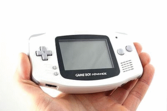
\includegraphics[width=\textwidth]{capitulos/capitulo1/modelo_a.png}
		\label{fig:modelo_a}
		\caption{Game Boy Advance}
	\end{subfigure}
	\hfill
	\begin{subfigure}[h]{0.3\textwidth}
		\centering
		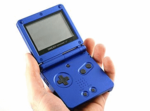
\includegraphics[width=\textwidth]{capitulos/capitulo1/modelo_b.png}
		\label{fig:modelo_b}
		\caption{Game Boy Advance SP}
	\end{subfigure}
	\hfill
	\begin{subfigure}[h]{0.3\textwidth}
		\centering
		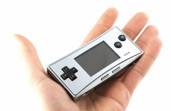
\includegraphics[width=\textwidth]{capitulos/capitulo1/modelo_c.png}
		\label{fig:modelo_c}
		\caption{Game Boy Advance Micro}
	\end{subfigure}
	\caption{Game Boy Advance, Game Boy Advance SP y Game Boy Advance Micro.}
	\label{fig:modelos}
\end{figure}


Entre los factores que contribuyeron a su éxito se incluyen la retrocompatibilidad con la generación de consolas previa de Nintendo, su precio asequible, la calidad de los juegos que desarrollaban las {\it third-party}\footnote{Se conoce como third-party a los juegos desarrollados por una entidad ajena a la compañía propietaria de la plataforma en la que se publican.} o la propia Nintendo y la relativa novedad que todavía tenía el mercado de consolas portátiles. Gracias a todos estos factores, la compañía japonesa prácticamente disfrutó de un monopolio en el mundo de las consolas portátiles\footnote{https://www.theverge.com/2019/4/19/18507409/nintendo-game-boy-competitors-nokia-sony-bandai} (esto se aplica tanto para la Game Boy original como para la Advance). \\ \\

\section{Explicación y objetivos del proyecto}\label{sec:objs}

En este Trabajo Fin de Grado se programará un {\bf juego para la consola Game Boy Advance}, que funcionará en el hardware original\footnote{Se probará con una Nintendo DS Lite, consola retrocompatible con la Game Boy Advance.} y en emuladores. Es importante destacar este aspecto porque el hecho de que un juego funcione en un emulador no garantiza que funcione también en el hardware original. Comentaremos algunos ejemplos de situaciones de este tipo a lo largo del trabajo.

Para poder realizar el proyecto correctamente se precisarán {\bf conocimientos del lenguaje de programación C aplicados a máquinas de propósito específico}. Estos deberán complementarse con un {\bf conocimiento de la arquitectura y funciones propias de la Game Boy Advance}. De forma adicional, dado que el trabajo se especializa en un área como es la de los videojuegos, será necesario {\bf familiarizarse con las técnicas profesionales de desarrollo de videojuegos}. Se espera poder conseguir un producto acorde con la calidad que ha ofrecido durante años la comunidad {\it homebrew}. Algo a destacar en este aspecto es la integración de archivos multimedia para su uso en el producto final. Entre los contenidos que se utilizarán se incluyen tanto {\it sprites}\footnote{Imagen asignada a un objeto/personaje de un videojuego.} como pistas de audio. Finalmente, el trabajo también requerirá del {\bf uso de métricas de rendimiento} durante el desarrollo para poder evaluar el software escrito y tomar decisiones en base a los resultados obtenidos.

En la siguiente lista se muestra  un resumen de los objetivos parciales anteriormente planteados, y derivados del objetivo principal de crear un juego para la Game Boy Advance (abreviada normalmente como GBA):

\begin{itemize}
	\item Aprendizaje de la arquitectura de la Game Boy Advance.
	\item Adquisición de conocimientos de desarrollo para máquinas de propósito específico.
	\item Ampliación práctica del conocimiento sobre programación en lenguaje C.
	\item Familiarización con las técnicas profesionales de desarrollo de videojuegos.
	\item Aplicación de técnicas de programación eficiente apoyadas en medidas de rendimiento (benchmarking) para comparar estrategias y soluciones a un mismo problema.
\end{itemize}

\section{Justificación e Intereses}

La idea de desarrollar un juego para una consola antigua, descatalogada desde hace más de una década, puede parecer un tanto peculiar como proyecto. Sin embargo, se puede justificar en base a diversos motivos. Uno de ellos es la arquitectura ARM\cite{bib:arm_book} de la máquina escogida, cuya relevancia no deja de aumentar actualmente. Otra razón es el atractivo docente de la propia consola, que permite estudiar, en un mismo dispositivo, muchos conceptos presentes en los planes de estudio del Grado en Ingeniería Informática \cite{bib:paper_2}. Igualmente, el trabajo no deja de precisar del esfuerzo y dedicación que cualquier proyecto de software requiere. Las labores de planteamiento, realización y gestión siguen estando presentes, e incluso se pueden llegar a dificultar dadas las peculiaridades que presenta un dispositivo de este tipo. Para poder realizar un proyecto de este estilo, el programador tendrá que involucrarse tanto en los aspectos más técnicos que trae consigo la programación de un dispositivo empotrado, como el diseño de funcionalidades con las que el usuario interactuará y que son ajenas a la programación (por lo menos de forma directa), como son el diseño de menús, personajes, niveles y controles del juego.

Además, el interés no solo procede de las dificultades que presentará la realización del trabajo, sino del dispositivo en sí. A título personal, el autor de este trabajo ha estado desde su infancia en contacto con consolas del fabricante nipón. Vivió incluso el final de la época de esplendor de la GBA. Por este motivo, poder desarrollar ahora software para esta plataforma supone un importante factor motivador. De forma complementaria, el desarrollo de software para sistemas empotrados siempre ha sido otro tema de interés para el autor dada su experiencia previa con microcontroladores ESPRESSIF\cite{doi:10.1177/0020294019857748} y Arduino. De hecho, desarrolló para el primero un pequeño juego, por lo que la transición a la Game Boy Advance se podría considerar el siguiente paso a seguir para continuar afianzando los conocimientos adquiridos.

Otro aspecto que motiva la realización de este trabajo, y que puede parecer contradictorio dada la naturaleza del dispositivo, es la disponibilidad del producto final para una infinidad de plataformas. Tal y como ya se mencionó, el software desarrollado podrá ejecutarse realmente en casi cualquier dispositivo actual gracias a la popularidad de la emulación.

En base a lo expuesto, podemos concluir que la realización del proyecto supone una motivación personal para el autor. Es además una propuesta bastante original en comparación a otros trabajos de este tipo aunque tenga las mismas exigencias a efectos prácticos. Igualmente, el resultado se podrá usar sin problemas en entornos actuales a pesar de estar destinado a una máquina descatalogada. Por consiguiente, se considera una forma perfecta de certificar los conocimientos y competencias adquiridas durante el Grado en Ingeniería Informática.

\section{Planificación del proyecto}
En este apartado se mostrarán las tareas a realizar y su planificación para completar los objetivos propuestos en la sección \ref{sec:objs}. La realización de las tareas se hará de modo que se siga una \textbf{estrategia de desarrollo} similar al \textbf{Ágil} (metodología popular en la industria de videojuegos \cite{bib:paper6,bib:agile_course}), en la que existirán varias iteraciones y prototipos del juego. Cada nueva iteración tendrá como base el \textit{feedback} y conocimientos adquiridos en la iteración anterior con el objetivo de conseguir un producto final pulido y acorde con los objetivos establecidos. Las diferentes fases de cada iteración se pueden observar en la Figura \ref{fig:agile}.

\begin{figure}[h]
	\centering
	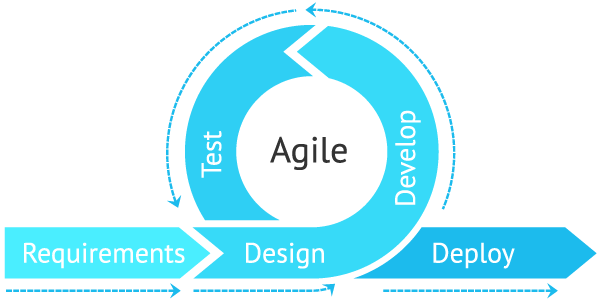
\includegraphics[width=.4\textwidth]{capitulos/capitulo1/agile.png}
	\caption[Metodología ágil]{Metodología ágil. Imagen de \url{devcom.com}.}
	\label{fig:agile}
\end{figure}

En su forma más simplificada, cada iteración repetirá el proceso del modelo de desarrollo en cascada, con la diferencia de que la metodología ágil no requiere acabar completamente cada fase. Por lo tanto, una vez planteado el proyecto y sus especificaciones (\textit{Requirements} en la Figura \ref{fig:agile}), las fases restantes se compondrán de las siguientes etapas:

\begin{enumerate}
	\item Diseño: Teniendo en cuenta los objetivos del proyecto, se diseñarán nuevas especificaciones y funcionalidades a implementar en la iteración actual.
	\item Desarrollo: Se implementará lo especificado en la fase anterior.
	\item Pruebas: Se evaluará lo desarrollado en el punto 2, comprobando que funciona acorde a lo esperado, tanto a nivel de programación, como a nivel conceptual, siendo habitual la prueba por parte del usuario final.
	\item Revisión: A pesar de que normalmente se incluye en la fase de Pruebas, esta fase merece una mención aparte. Teniendo en cuenta, los constantes cambios que se realizan en este tipo de proyectos, es necesario revisar lo desarrollado y decidir si el proyecto sigue acorde con la idea original. Los ajustes a realizar se identificarán en esta fase y se tendrán en cuenta para la próxima iteración.
\end{enumerate}

Con una versión del producto acabada, los desarrolladores publicarán la iteración con la posibilidad de empezar a revisitar las fases descritas anteriormente para lanzar una versión mejorada o con más funcionalidades \cite{bib:agile_course}.

Dado que el proyecto se comenzó con un escaso conocimiento sobre las funcionalidades y arquitectura de la Game Boy Advance, se aprovecharon las iteraciones para conocer las diferentes opciones y características del dispositivo. Por ejemplo, en la primera iteración se analizaron las posibilidades a nivel gráfico que ofrece el dispositivo, mientras que durante la segunda iteración se exploraron las posibilidades que ofrece el procesador, a nivel de audio. En total, se utilizaron un total de 4 iteraciones, también denominadas \textit{sprints}, para realizar el proyecto.

Al combinar los \textit{sprints} junto con las demás tareas ``no iterables'' se obtiene un proyecto el cual ha requerido \textbf{300 horas en total}. Las tareas en cuestión se distribuyen de la siguiente manera:

\begin{enumerate}
	\item \textbf{Estudio de la arquitectura de la Game Boy Advance (40 horas)}: Estudio de la arquitectura con ayuda de la documentación recogida en la bibliografía.
	\item \textbf{Asimilación de técnicas de programación específicas (18 horas)}: Estudio de proyectos de código abierto para Game Boy Advance con los que aprender estrategias de desarrollo de calidad contrastada para esta plataforma.
	\item \textbf{\textit{Sprint} (49.25 horas)}: Desarrollo del proyecto. A continuación, se desglosan y describen las tareas de cada uno de los 4 \textit{sprints} que se realizan, para un total de 197 horas.
		\begin{itemize}
			\item \textbf{Reuniones con los tutores (20 horas)}: Reuniones con el profesorado para definir los requisitos del proyecto, seguir su desarrollo y resolver posibles dudas.
			\item \textbf{Diseño de los niveles del juego (17 horas)}: Estudio de niveles existentes en diferentes juegos para inspiración propia.
			\item \textbf{Diseño y creación de recursos (5 horas)}: Elaboración, mediante herramientas como Adobe Photoshop o GIMP, de elementos del juego como sprites e iconos. Dada la poca familiaridad con el software de dibujo y la falta de experiencia en este campo, se propuso optar por diseños \textit{Open Source} para realizar el juego. A pesar de trabajar con recursos ya existentes, se siguen necesitando 5 horas, dado que será necesario convertirlos a formatos que la consola pueda ``entender''.
			\item \textbf{Implementación (105 horas)}: Programación del juego deseado acorde a las especificaciones propuestas en las tareas de ``Diseño''. Esta tarea es la más exigente, por lo que se le asignaron un mayor número de horas que a las restantes. 
			\item \textbf{Evaluación del producto (50 horas)}: Análisis del resultado obtenido en la tarea de ``Implementación'' para la identificación y solución de errores y aplicación de mejoras.
		\end{itemize}
	\item \textbf{Elaboración de memoria (45 horas)}: Redacción de un informe que describa todo el trabajo desarrollado en las distintas facetas.
\end{enumerate}

La temporización de las tareas mostradas se puede observar en la Tabla~\ref{tab:iteraciones}. Por su parte, el diagrama de Gantt, que refleja visualmente los datos mostrados en la Tabla~\ref{tab:iteraciones}, quedaría como se muestra en la Figura~\ref{fig:gantt}. La Tabla se ha calculado estimando unas 2 horas por día dedicadas al proyecto. 

\begin{table}[h]
	\centering
	\begin{tabular}{| l | l | l | l |}
		\hline
		\textbf{Tarea} & \textbf{Duración} & \textbf{Inicio} & \textbf{Fin} \\ \hline
		Estudio arquitectura GBA & 40 horas & Lunes 08/02/21 & Sábado 27/02/21 \\ \hline
		Estudio técnicas de programación & 18 horas & Domingo 28/02/21  & Lunes 08/03/21\\ \hline
		Sprint 1 & 49.25 horas & Martes 09/03/21 & Sábado 03/04/21 \\ \hline
		Sprint 2 & 49.25 horas & Sábado 03/04/21 & Miércoles 28/04/21 \\ \hline
		Sprint 3 & 49.25 horas & Miércoles 28/04/21 & Domingo 23/05/21 \\ \hline
		Sprint 4 & 49.25 horas & Domingo 23/05/21 & Jueves 17/06/21 \\ \hline
		Elaboración del informe & 45 horas & Jueves 17/06/21 & Viernes 09/07/21 \\ \hline
		Entrega & - & \multicolumn{2}{c|}{Viernes 09/07/21} \\ \hline
	\end{tabular}
	\caption{Temporización por iteración.}
	\label{tab:iteraciones}
\end{table}

\begin{figure}[t]
	\centering
	\rotatebox[origin=c]{270}{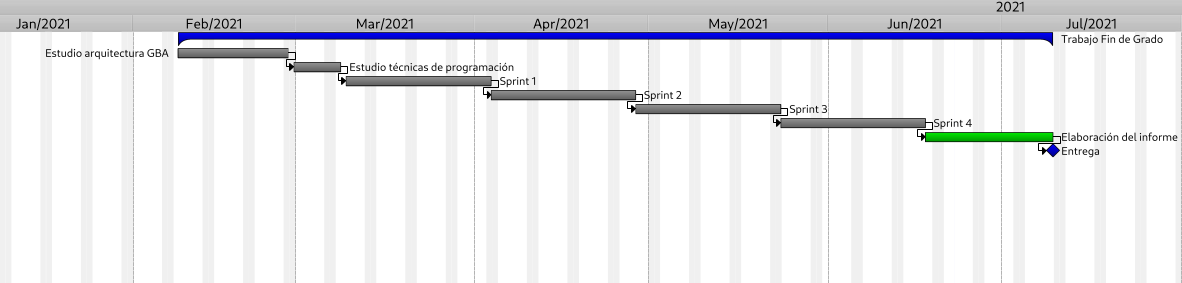
\includegraphics[width=20cm]{capitulos/capitulo1/gantt_3.png}}
	%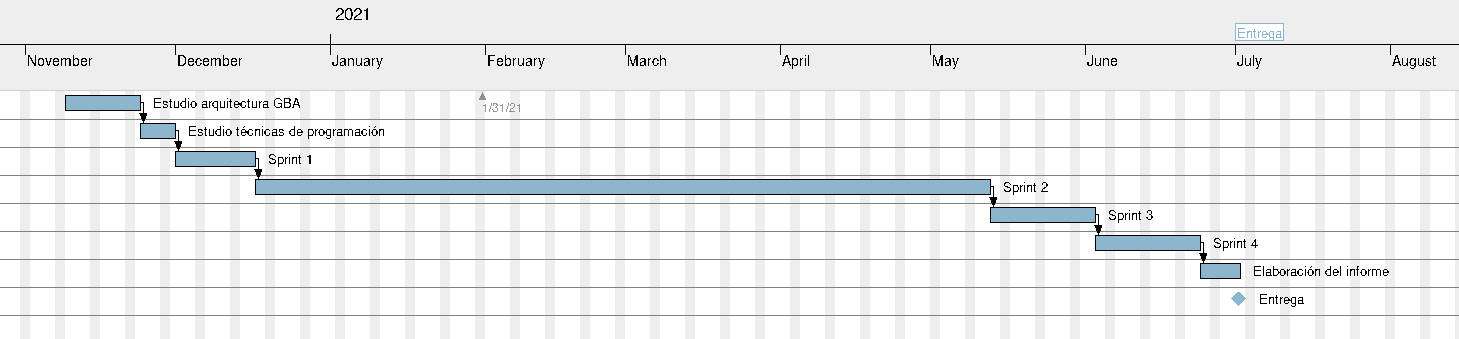
\includegraphics[height=1.2\textwidth]{capitulos/capitulo1/gantt_2.png}
	\caption{Diagrama de Gantt.}
	\label{fig:gantt}
\end{figure}
\FloatBarrier{}

\section{Recursos utilizados}
En esta sección se describirán las herramientas utilizadas para poder realizar satisfactoriamente el proyecto. Se ha considerado oportuno clasificarlas en los subapartados de Lenguajes de programación, Control de versiones, Editores, Herramientas gráficas y de audio, Herramientas de planificación, Emuladores y Hardware.

\subsection{Lenguajes de programación}
Como se mencionó en el punto \ref{sec:objs}, para llevar a cabo el proyecto se va a \textbf{programar en C}. Aunque actualmente existen varias formas de desarrollar un juego para la Game Boy Advance (a partir de C++ y Rust por ejemplo), se seguirá apostando por C, dada la documentación y su uso extendido en la comunidad \textit{homebrew}. El estándar utilizado para el proyecto será el ``GNU17'', el que usa GCC por defecto\footnote{https://gcc.gnu.org/onlinedocs/gcc-11.1.0/gcc/Standards.html}, que es también el compilador empleado en este proyecto. Además, para simplificar el proceso de compilación, se hará uso de la utilidad make.

\subsection{Control de versiones}
Para gestionar el código se hará uso del popular software de control de versiones \textbf{Git}. Además, para alojar el proyecto se utilizará un servidor privado (de modalidad gratuita) de \textbf{\href{https://github.com/}{GitHub}}.

\subsection{Editores}
Dada la necesidad de programar y escribir el informe final en diferentes máquinas, se optará por utilizar editores multiplataforma. Para programar se hará uso de \textbf{Vim} y \textbf{Visual Studio Code}. El primero es adecuado para editar rápidamente archivos y automatizar ciertas tareas, mientras que el segundo es muy eficaz para trabajar simultáneamente con diversos archivos.

En cuanto a la escritura del informe, se hará uso de \textbf{\TeX maker}, que proporciona una interfaz simple y cómoda para personas que no cuenten con mucha experiencia escribiendo en \LaTeX.

\subsection{Herramientas gráficas y de audio}\label{sec:herr_graficas}
Teniendo en cuenta la naturaleza del dispositivo para el que se programará, será necesario convertir los diferentes recursos gráficos a un formato especial. \textbf{Grit} y \textbf{SuperFamiconv}, herramientas creadas específicamente para la conversión de imágenes a un formato reconocible por la Game Boy Advance, se utilizarán para adaptar recursos conocidos como \textit{sprite sheets} y \textit{tile sets} (los cuales se explicarán y se verán con más detenimiento en el punto \ref{sec:ppu}).

Independientemente de si los recursos gráficos son de terceros o propios, la mayoría de las veces será necesario retocar las imágenes antes de convertirlas. Para ello será necesario \textbf{Pixelorama}, editor específicamente diseñado para trabajar con \textit{sprites}.

Para generar los fondos que utilizará el juego, se hará uso de \textbf{Tiled}, uno de los editores de niveles \textit{open source} más populares. Su uso se mostrará en el punto \ref{sec:ppu}.

Por último, para convertir música utilizada para el juego en un formato reconocible para el dispositivo se utilizará \textbf{Audacity}.

\subsection{Herramientas de planificación}
Para planificar cada una de las tareas del proyecto así como calcular su distribución se utilizará \textbf{Plan}, de la suite de aplicaciones Calibra. Por otro lado, \textbf{Trello} se utilizará para clasificar las tareas del proyecto en cada uno de los \textit{sprints} a realizar.

\subsection{Emuladores}
Tras explicar las herramientas necesarias para poder desarrollar el proyecto, pasamos a aquellas que nos permitirán probarlo y ejecutarlo. Las escogidas para este proyecto son los emuladores mGBA y No\$GBA. Del primero se destaca su activo desarrollo y el ser multiplataforma, mientras que del segundo se pueden resaltar las opciones de depuración que ofrece al usuario.

%\begin{figure}[h]
%    \centering
%    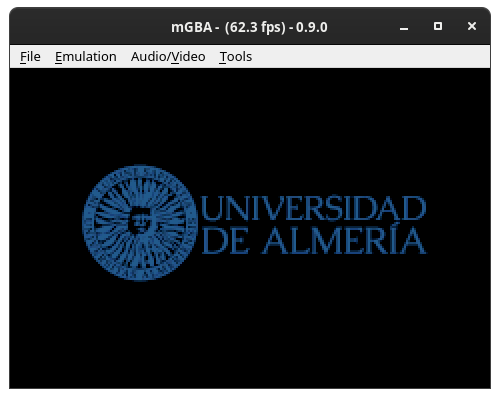
\includegraphics[width=.5\textwidth]{capitulos/capitulo1/mgba.png}
%    \caption{El emulador mGBA.}
%    \label{fig:mgba}
%\end{figure}
%\FloatBarrier

\subsection{Hardware}
Finalmente, pasamos a los recursos que ejecutarán las versiones finales de nuestro proyecto (también las versiones de desarrollo, pero con menor frecuencia). En este caso, al no disponer de una consola Game Boy Advance original, se hará uso de una consola retrocompatible, la \textbf{Nintendo DS Lite} (véase la Figura \ref{fig:nintendo_ds}).

Lamentablemente, la consola no admite cargar directamente software \textit{homebrew}. Por este motivo, se utilizará un cartucho \textbf{Supercard} (véase la Figura \ref{fig:supercard}), que permitirá, mediante una tarjeta microSD, ejecutar el software generado.

\begin{figure}[h]
	\centering
	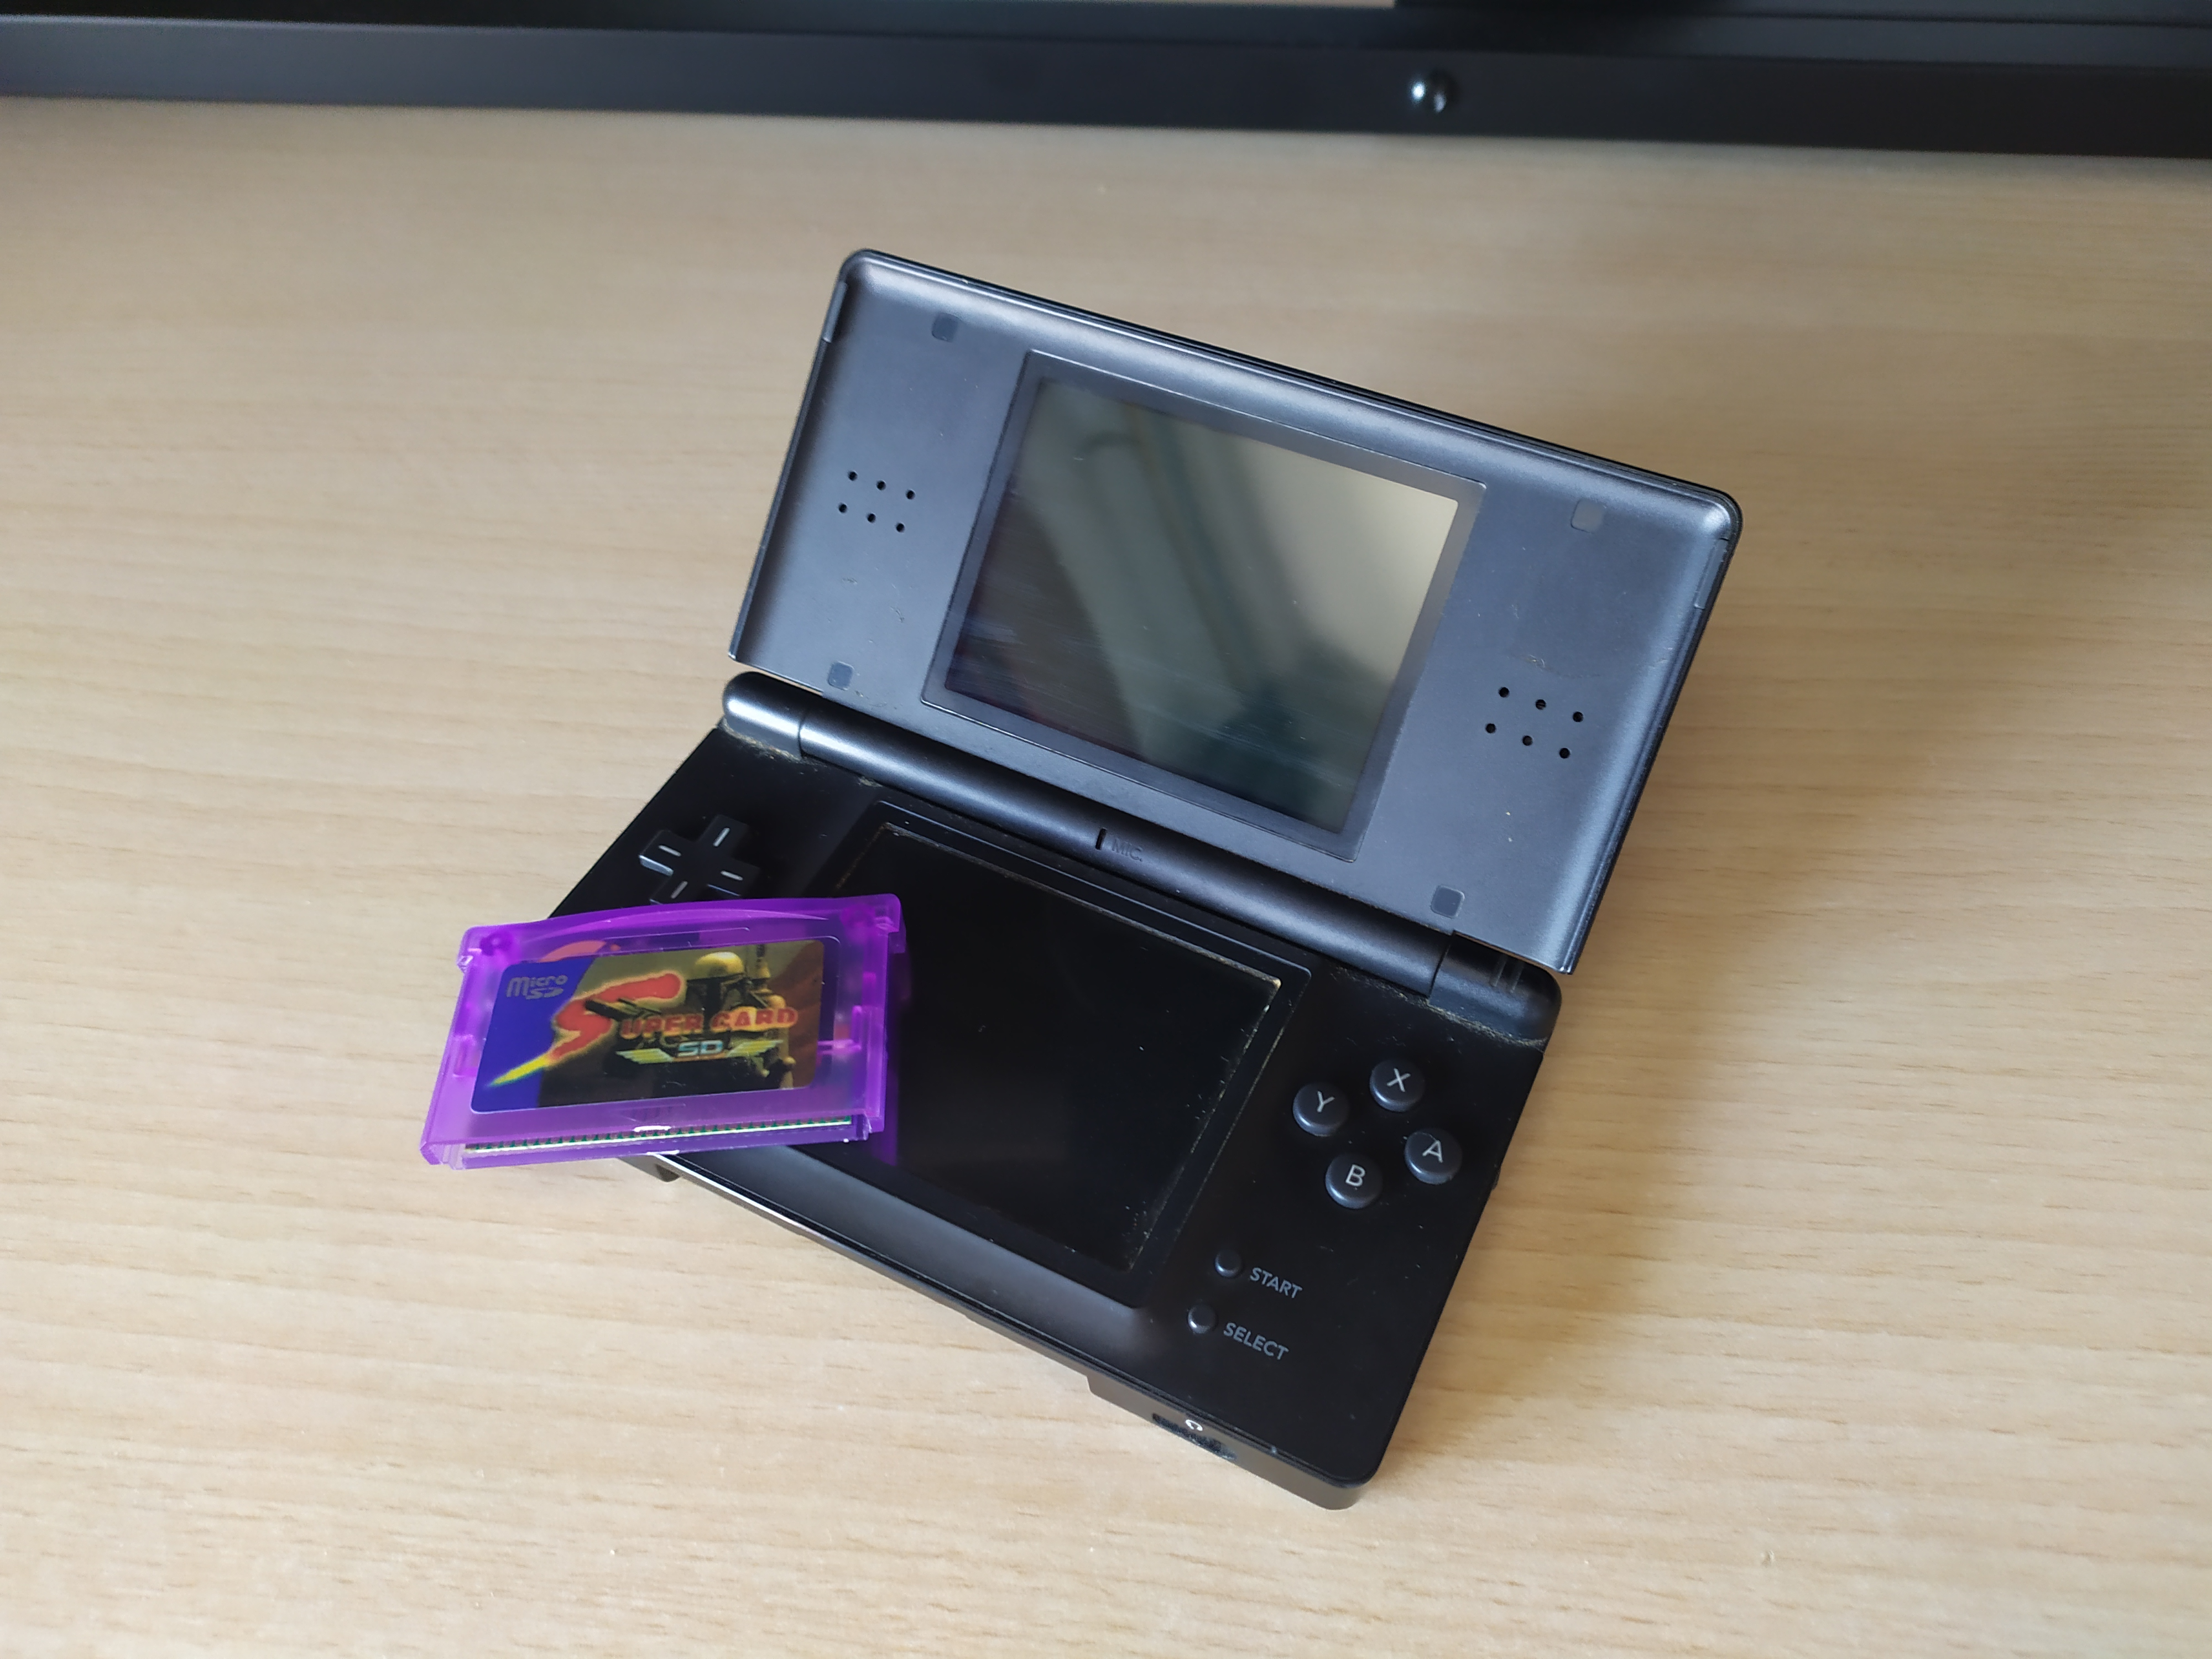
\includegraphics[height=7cm]{capitulos/capitulo1/nintendo_ds.jpg}
	\caption{Consola retrocompatible con la Game Boy Advance, la Nintendo DS Lite.}
	\label{fig:nintendo_ds}
\end{figure}

\vspace{1cm}

\begin{figure}[h]
	\centering
	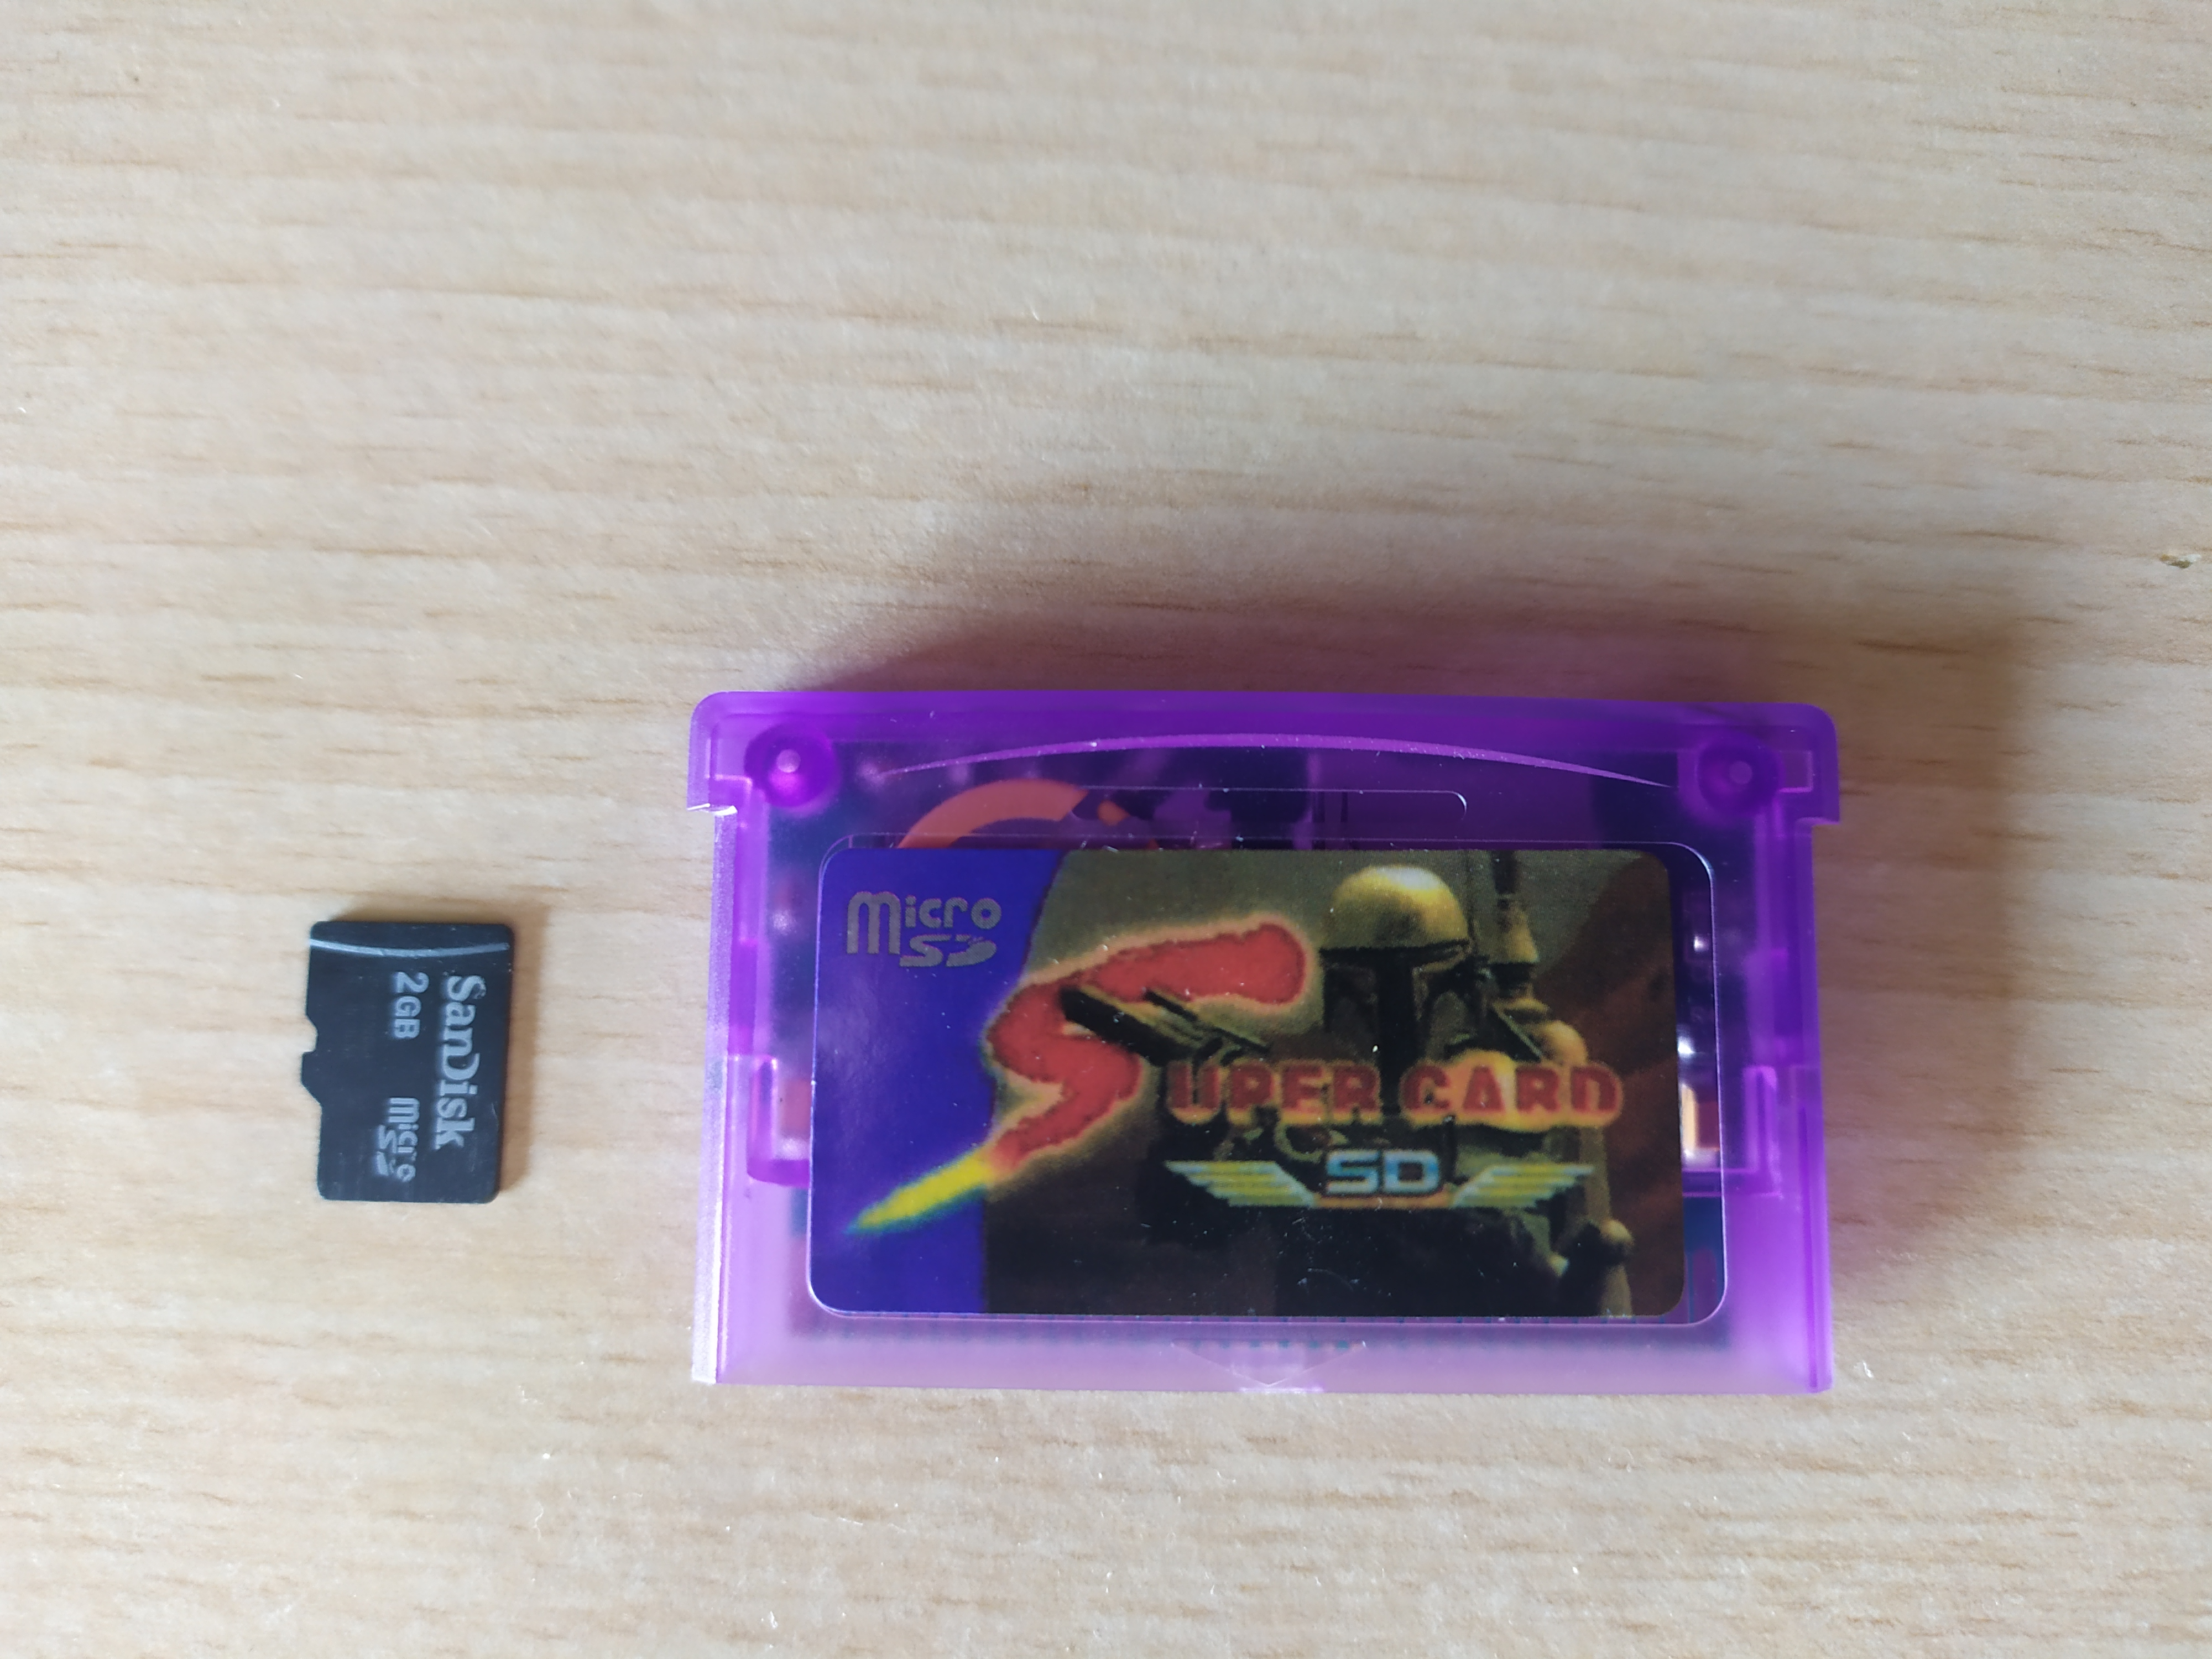
\includegraphics[height=6cm]{capitulos/capitulo1/supercard.jpg}
	\caption{Cartucho \textit{Supercard}.}
	\label{fig:supercard}
\end{figure}
\FloatBarrier

\section{Estructura del proyecto}
Este documento tiene como finalidad mostrar la solución desarrollada al problema propuesto, comentando a su vez las diversas características que tiene la Game Boy Advance. Dado que será necesario conocer varios conceptos antes de comentar el desarrollo del juego, la estructura del proyecto comenzará describiendo la arquitectura de la GBA y las opciones que ofrece.

En el Capítulo \ref{sec:arquitectura} se comentarán brevemente las características de los dos procesadores que utiliza la consola nipona y el papel que tiene cada uno en el dispositivo.

Seguidamente, se expondrán los registros principales y las funciones de cada uno. Entre ellas se encuentran, por ejemplo, la configuración de la pantalla y del sonido, las transferencias de acceso a directo a memoria y la comunicación con otros dispositivos.

Teniendo una idea de los registros que el desarrollador necesitará conocer para programar en el dispositivo, se explicarán los modos que ofrece la unidad de procesamiento de imágenes de la consola (\textit{PPU} ó \textit{Picture Processing Unit}). Se combinará la explicación de los diferentes modos con pequeñas demostraciones para facilitar la comprensión. Además, se introducirán al lector algunos conceptos matemáticos necesarios para comprender el funcionamiento de algunas de las funciones de la \textit{PPU}.

Partiendo de la base previa, en el Capítulo \ref{sec:desarrollo}, se detallarán los requisitos y especificaciones del proyecto, entre los que se incluirán varios diagramas. De forma adicional, se resaltarán algunos aspectos del desarrollo que distinguen a la Game Boy Advance con respecto a otros dispositivos.

En la fase final del informe, en concreto en el Capítulo \ref{sec:final}, se presentará la solución desarrollada para el proyecto, describiéndose el funcionamiento del juego. Se mostrará también cómo se ha probado el software en el hardware real, detallando el procedimiento a seguir.

Una vez descrito el estado actual del juego, en el Capítulo \ref{sec:conclusion} se expondrán las conclusiones detallando los conocimientos adquiridos y la experiencia de desarrollar un juego para la Game Boy Advance. Adicionalmente, se comentarán varias de las funcionalidades y mejoras descartadas para el proyecto en la fase de prototipado (de cada iteración) que podrán servir como líneas de trabajo en un futuro.

Finalmente, en los apéndices se incluirán información adicional de los registros y funciones del sistema, estructura del proyecto a nivel de código, varias imágenes mostrando el juego en funcionamiento y varios \textit{scripts} utilizados para facilitar el desarrollo del producto final.

\chapter{Arquitectura de la Game Boy Advance}\label{sec:arquitectura}

Con un procesador RISC como corazón del sistema, la Game Boy Advance tiene unas especificaciones modestas, similares a lo que veríamos en los dispositivos embebidos de hoy en día. El dispositivo cuenta con un unidad ARM7TDMI de 32 bits como procesador principal. Tiene también un coprocesador el cual fue utilizado en la iteración anterior de la consola, el Sharp SM83 (basado en el set de instrucciones 8080 de 8 bits). Esto permite a la consola jugar, de forma nativa, a juegos desarrollados para la Game Boy original \cite{bib:rodrigo}. 

Estos dos procesadores residen en el mismo SoC (véase en la Figura \ref{fig:circuit}) y permiten a la consola ejecutarse en varios modos. Podemos distinguir los siguientes:
\begin{itemize}
\item El \textbf{modo ARM}, que hace que el procesador funcione a 16.78 MHz, manejando instrucciones de 32 bits.
\item El \textbf{modo THUMB}, reservado para optimizar partes del código. En este modo la consola también funciona a una frecuencia de 16.78 MHz, pero solo acepta instrucciones de 16 bits.
\item El \textbf{modo CGB} (Color Game Boy), que utiliza el coprocesador mencionado anteriormente para ejecutar código escrito para la Game Boy Color original (la frecuencia puede variar entre 4.2 MHz y 8.4MHz).
\item El \textbf{modo DMG} (Dot Matrix Game), similar el modo anterior, aunque esta vez limitado a 4.2 MHz. Está reservado para su uso en juegos programados para la Game Boy con pantalla monocromática.
\end{itemize}

\begin{figure}[t]
    \centering
    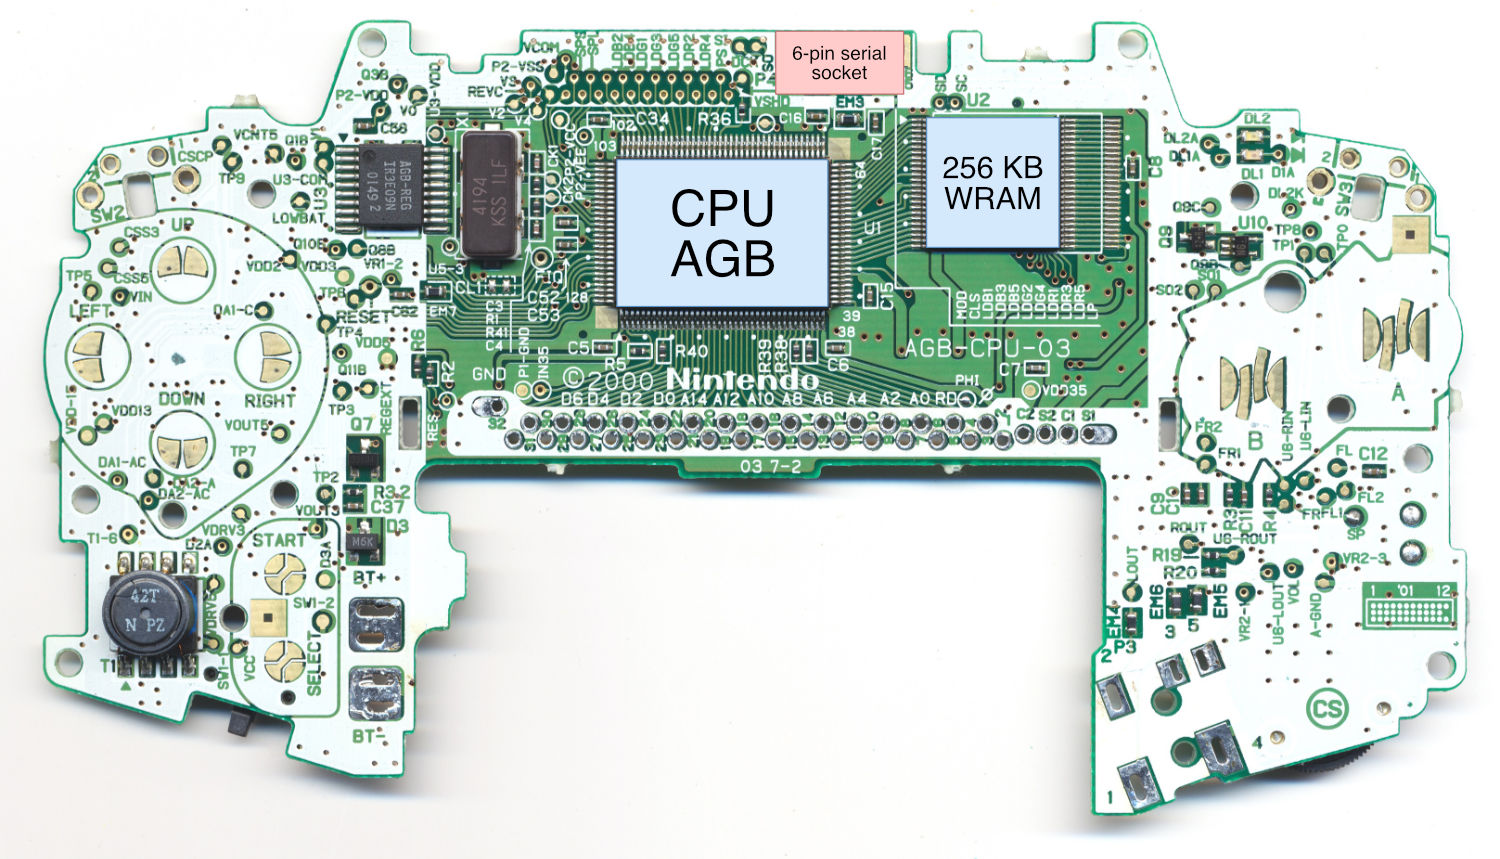
\includegraphics[width=.8\textwidth]{capitulos/capitulo2/circuit.jpg}
    \caption{El circuito de la Game Boy Advance \cite{bib:rodrigo}.}
    \label{fig:circuit}
\end{figure}


Es importante mencionar que ambos procesadores no pueden ejercer la función de procesador central simultáneamente. Por ende, el programador puede cambiar del modo ARM al THUMB y viceversa, pero no de un modo que use el procesador ARM7 a otro que utilice el Sharp SM83 \cite{bib:gbatek}.

La consola cuenta con el mapa de memoria detallado en la Tabla~\ref{tab:mapa} que, dependiendo a que sección se accede, tiene buses de 32, 16 u 8 bits. La práctica de tener buses de diferentes tamaños es común en consolas, incluso de sobremesa como la PlayStation 2~\cite{bib:comp_arch_quant}.

\begin{table}[h]
	\centering
	\begin{tabular}{| l | l | l | l |}
		\hline
		\textbf{Nombre} & \textbf{Sección} & \textbf{Tamaño} & \textbf{Bus} \\ \hline
		ROM del sistema & 0x00000000-0x00003FFF & 16 KB & 32 bits \\ \hline
		RAM externa (On-board RAM) & 0x02000000-0x0203FFFF & 256 KB\tablefootnote{A pesar de tener disponible 256 KB, la Game Boy reserva en los últimos 256 bytes datos que gestiona internamente, como el vector de interrupciones.} & 16 bits\\ \hline
		RAM interna (On-chip RAM) & 0x03000000-0x03007FFF & 32 KB & 32 bits \\ \hline
		RAM de IO & 0x04000000-0x040003FE & - & 32 bits \\ \hline
		RAM de paleta & 0x05000000-0x050003FF & 1 KB & 16 bits \\ \hline
		VRAM & 0x06000000-0x06017FFF & 96 KB & 16 bits \\ \hline
		Memoria de objetos & 0x07000000-0x070003FF & 1 KB & 32 bits \\ \hline
		ROM y flash del cartucho & 0x08000000-0x0DFFFFFF & $\leq$ 96 MB  & 16 bits \\ \hline
		SRAM del cartucho & 0x0E000000-0x0E00FFFF & $\leq$ 64 KB & 8 bits \\ \hline
	\end{tabular}
	\caption{Mapa de memoria de la Game Boy Advance.}
	\label{tab:mapa}
\end{table}


Los espacios que aparecen en la tabla anterior, entre la ROM del sistema y la RAM externa (en concreto, 0x00004000-0x01FFFFFF), son regiones que no se utilizan o en las que el programador no tiene que intervenir de ninguna manera \cite{bib:gba_manual}.

A continuación, comentaremos brevemente la función que se le da a cada sección.

\begin{itemize}
	\item \textbf{ROM del sistema}: Encabezando el mapa de memoria de la consola encontramos la ROM del sistema, la cual guarda, como su nombre indica, código inmutable del sistema. Contiene por ejemplo la BIOS y rutinas que el programador puede utilizar en su juego. Entre las rutinas incluidas se pueden distinguir algunas para calcular operaciones  aritméticas complejas y transformaciones afines, y otras para llevar a cabo funciones de descompresión, sonido, copia de memoria e interacción con otras consolas al conectarlas mediante el cable \textit{link}\footnote{La Game Boy Advance permitía jugar con hasta 4 personas mediante una conexión por cable.} (función conocida como \textit{multi-boot}).
	\item \textbf{RAM}: A continuación, después de la ROM, se encuentra la RAM de la consola (también conocida como EWRAM o External Work RAM), en la que se distinguen dos tipos. La primera región, posicionada en la dirección 0x02000000, reside fuera del SoC (véase la Figura \ref{fig:circuit}). Cuenta con un tamaño de 256 KB y un bus de 16 bits por el cual podemos considerar esta sección como la RAM ``lenta''. La siguiente región que encontramos en el mapa de memoria, la RAM interna, ofrece un bus completo de 32 bits, pero con un tamaño reducido (comparado con la RAM externa) de 32 KB. En la Figura \ref{fig:distribucion_1} se muestra la distribución y localización de la IWRAM y EWRAM. \\

	\begin{figure}[h]
	    \centering
	    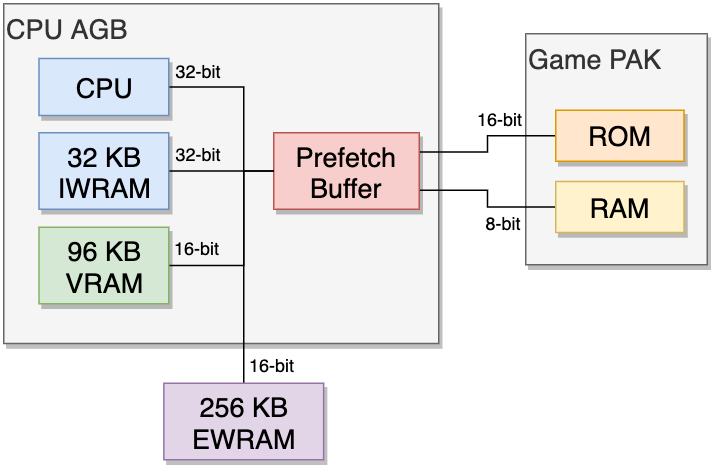
\includegraphics[width=.5\textwidth]{capitulos/capitulo2/distribucion.png}
	    \caption{Distribución de la memoria de la Game Boy Advance \cite{bib:rodrigo}.}
	    \label{fig:distribucion_1}
	\end{figure}

	\item \textbf{Registro de control de entrada y salida}: En la siguiente sección aparece ``mapeado'' el registro de control de entrada y salida en el que el programador puede consultar información (como las teclas que el usuario presiona) y modificar la configuración de la consola. Por ejemplo, en esta región se encuentran los valores que determinarán el tipo de gráficos que utilizará el juego.
	\item \textbf{RAM de paleta}: La RAM de paleta, o ``palette RAM'' en inglés, es la sección de memoria que cubre el espacio necesario para albergar las paletas de colores de los diferentes modos de vídeo y gráficos disponibles.
	\item \textbf{VRAM}: En la VRAM se almacenan los índices de la paleta de colores para referenciarlos. Además de esta función en algunos modos de la Game Boy Advance, la VRAM también contiene los objetos o píxeles que aparecerán en pantalla. Más adelante se darán más detalles.
	\item \textbf{Memoria de Objetos}: La memoria de objetos (OAM, de "Object Attribute Memory" en inglés), al igual que la RAM de paleta, se utiliza en unos modos concretos y se encarga de guardar los datos de objetos a mostrar, informalmente nombrados por el anglicismo {\it sprites}. Estos ``objetos'' son, normalmente, el texto y personajes que aparecen en los juegos 2D. Algunos de los atributos que maneja esta región son la posición, rotación, escala y tamaño. \\

	Las tres secciones descritas, RAM de paleta, VRAM y OAM, forman parte de la PPU (\textit{Picture Processing Unit}) de la Game Boy Advance. Esta se encarga de combinar y procesar la información almacenada en dichas regiones (qué información procesa  y cómo dependerá del modo de vídeo utilizado) para crear una imagen que el usuario pueda ver. La distribución de la PPU se observa en la Figura \ref{fig:distribucion_2}.

	\begin{figure}[h]
	    \centering
	    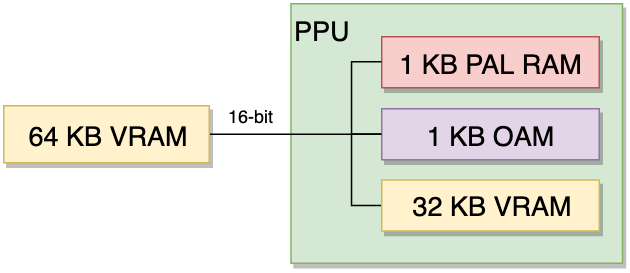
\includegraphics[width=.5\textwidth]{capitulos/capitulo2/ppu.png}
	    \caption{La PPU de la Game Boy Advance.}
	    \label{fig:distribucion_2}
	\end{figure}

	\item \textbf{ROM y SRAM del cartucho}: La última región en el mapa de memoria es la vinculada con el cartucho del juego, que se introduce en la ranura que ofrece la consola y funciona mediante una conexión paralela. La ejecución del juego empieza en esta dirección de memoria\footnote{Salvo en juegos multijugador, en ese caso la ejecución del juego comienza en las instrucciones localizadas en la RAM externa (0x02000000).}, la ROM del cartucho (0x08000000). Para que los jugadores puedan guardar sus partidas se dedican los últimas 64 KB, sección denominada SRAM \cite{bib:tonc,bib:gba_manual,bib:gbatek}.
\end{itemize}

Todas las zonas de memoria anteriores se pueden ver distribuidas en el diagrama del circuito de la consola, en la Figura \ref{fig:diagrama}.

\begin{figure}[h]
    \centering
    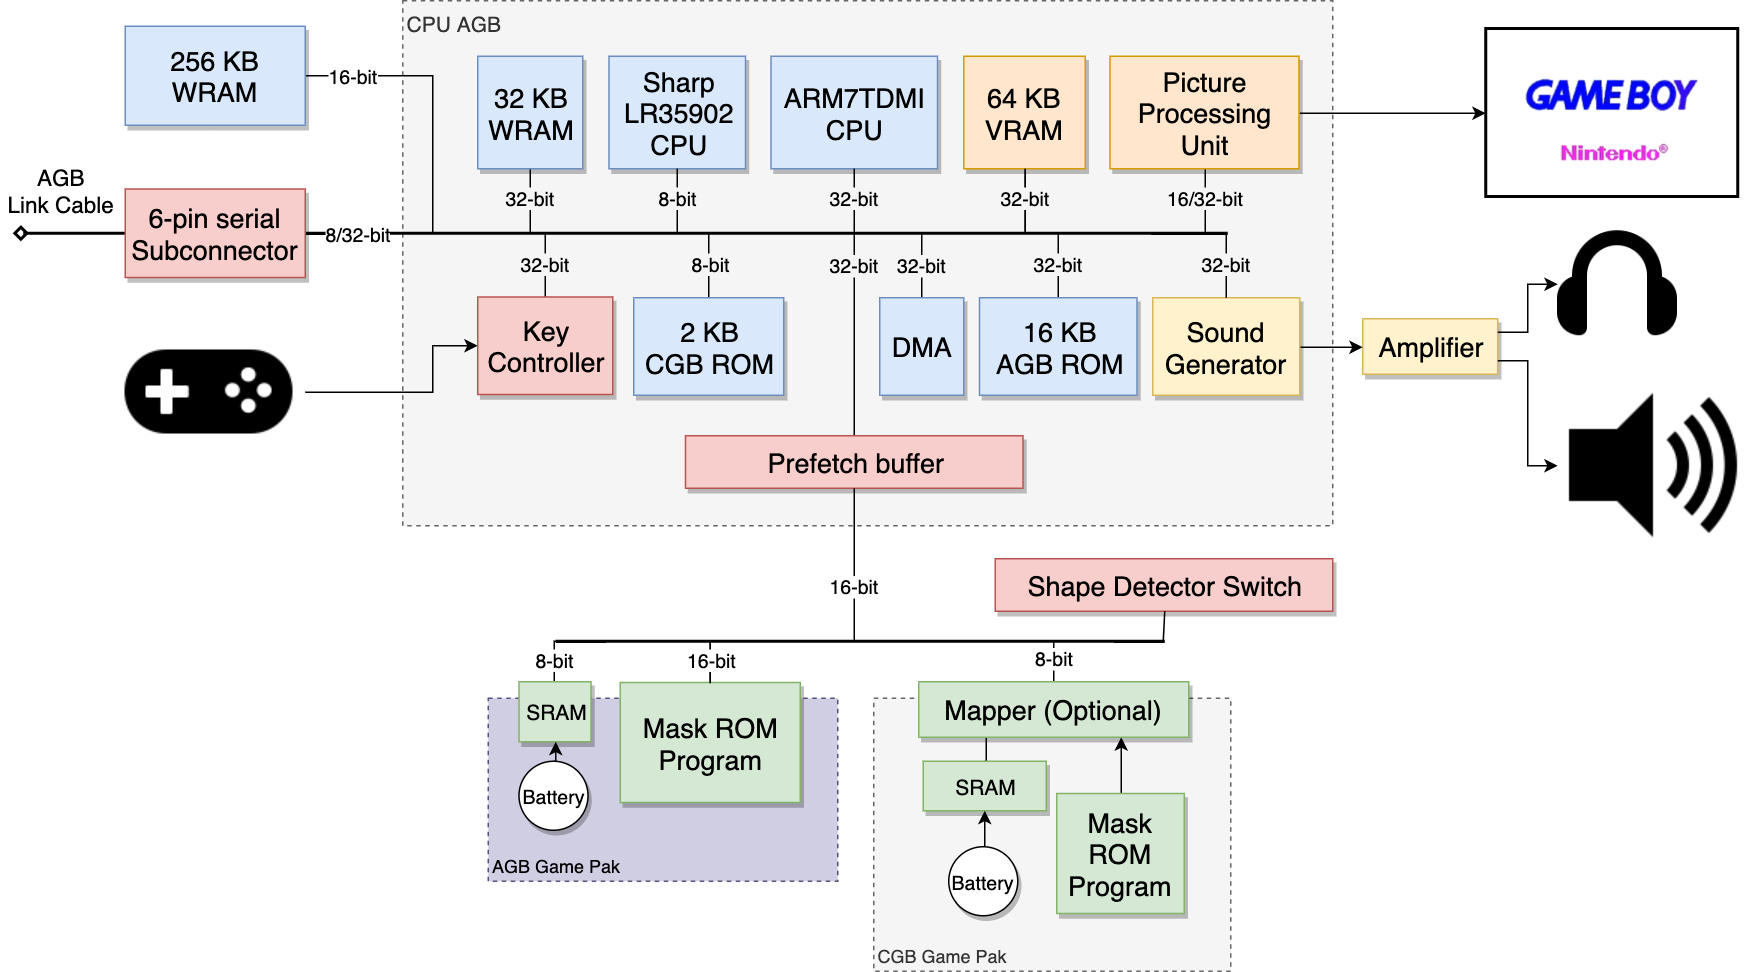
\includegraphics[width=.9\textwidth]{capitulos/capitulo2/diagram.png}
    \caption{Diagrama simplificado del circuito de la Game Boy Advance \cite{bib:rodrigo}.}
    \label{fig:diagrama}
\end{figure}
\FloatBarrier{}

\section{Procesador ARM7TDMI}
En este punto se incluyen los aspectos más importantes del procesador principal de la Game Boy Advance. Toda la información se puede encontrar en \cite{bib:arm} (el documento de referencia del procesador), complementada con detalles adicionales sobre el juego de instrucciones utilizado en \cite{bib:armv4_isa}.

Para cumplir con las exigencias de potencia computacional de la nueva generación de consolas portátiles, Nintendo, decidió diseñar un procesador basado en ARMv4, un  juego de instrucciones (ISA o \textit{Instruction Set Architecture} en inglés)  RISC. Las especificaciones del ISA nos dan una idea de las características del dispositivo:

\begin{itemize}
	\item \textbf{ARMv4} tiene un total de 37 registros de 32 bits, de los cuales 31 son generales y 6 son de estado. En la Game Boy existen diferentes modos. Cada uno de ellos tiene acceso a 17, o menos, de los registros disponibles. El acceso según el modo del procesador a los registros del sistema se describe en la Figura \ref{fig:registros_arm}. Es importante resaltar que, tal y como pasa con otros procesadores ARM, algunos de los 37 registros no son \textit{banked registers}, lo que significa que varios modos compartirán registros y, por lo tanto, los valores de estos pueden ser sobrescritos. \\

	Ignorando los modos privilegiados mostrados en la Figura \ref{fig:registros_arm} (\textit{FIQ, Supervisor, Abort, IRQ, Undefined}), los usos de los registros en el modo general (primera columna de la figura, \textit{System and User}) que controlará el programador son:

		\begin{itemize}
			\item Generales: Los registros considerados como generales son R0-R12. Sin embargo, mientras que el modo ARM tiene libertad total para acceder a cada uno de los 13, el modo THUMB solo puede acceder de R8 a R12 utilizando instrucciones específicas. 
			\item \textit{Stack Pointer}: El registro R13 se utiliza para guardar la dirección de la pila, esto se realiza por convención en el modo ARM, dado que también se puede utilizar como un registro de uso general. No obstante, en el caso del modo THUMB debe utilizarse como \textit{Stack Pointer}.
			\item \textit{Link Register} y \textit{Program Counter}: R14 se reserva para guardar la dirección de memoria de R15 (\textit{Program Counter}) al realizar una instrucción de salto, también conocida como instrucción de \textit{branch}. No obstante, como ocurre con el registro R13, en caso de no usar este tipo de instrucciones, el modo ARM permite utilizar el registro para uso general. Otra diferencia a tener en cuenta entre los dos modos es el valor del contador del programa, el registro R15, que almacena el valor del contador en los bits 2-31 en el modo ARM y 1-31 en el modo THUMB.
			\item CPSR y SPSR: El registro CPSR (\textit{Current Program Status Register}), accesible en todos los modos, almacena datos como el estado del procesador e información de control como el resultado de instrucciones CMP. En los modos privilegiados encontramos un registro adicional además de los 17 registros explicados en el punto anterior, denominado SPSR (\textit{Saved Program Status Register}), en el que se guardan los valores del registro CPSR en caso de excepción.
		\end{itemize}

\begin{figure}[t]
    \centering
    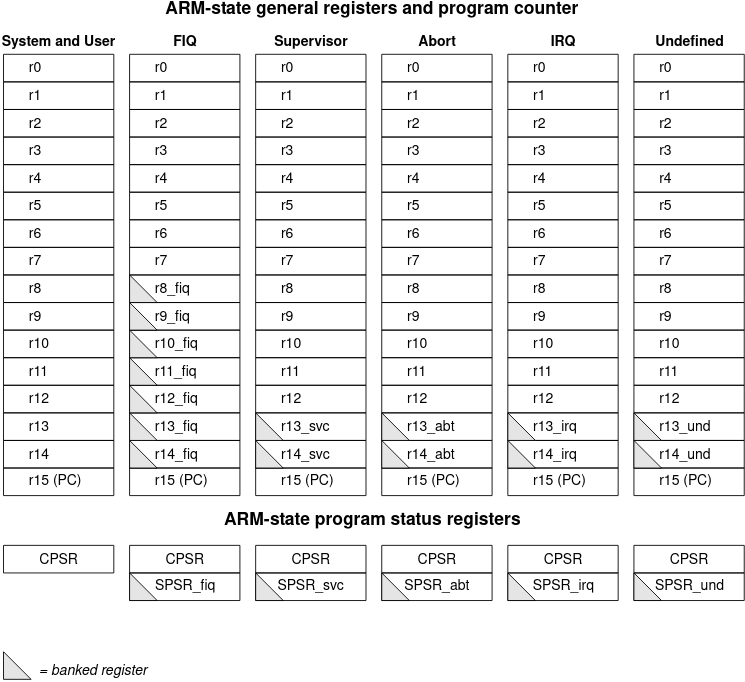
\includegraphics[width=.8\textwidth]{capitulos/capitulo2/registros.png}
    \caption{Registros por modo del procesador ARM7TDMI.}
    \label{fig:registros_arm}
\end{figure}

Las limitaciones que se comentaron anteriormente con el modo THUMB del procesador y los efectos que tiene en el acceso de los registros quedan representados en la Figura \ref{fig:registros_thumb}.

\begin{figure}[h]
    \centering
    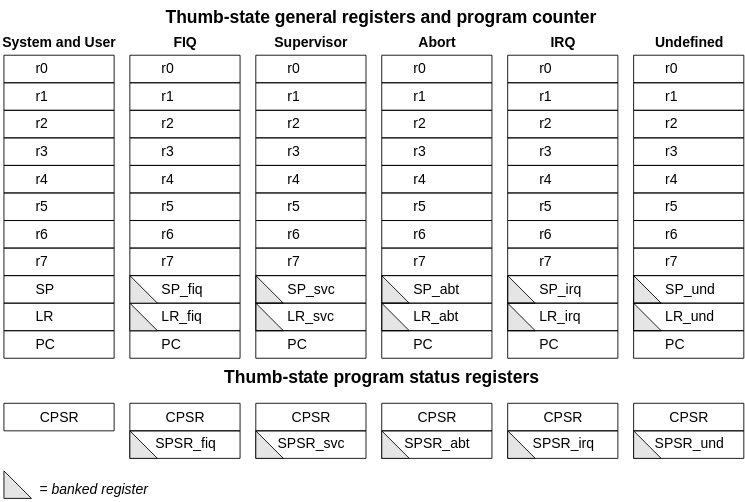
\includegraphics[width=.8\textwidth]{capitulos/capitulo2/registros_thumb.png}
    \caption{Registros por modo del procesador ARM7TDMI cuando este utiliza el set de instrucciones THUMB.}
    \label{fig:registros_thumb}
\end{figure}

\item La consola utiliza un juego de instrucciones \textbf{load-store} en el cual todas las operaciones aritméticas que operan en memoria tienen que realizarse mediante instrucciones load. Este \textit{ISA} permite también el uso de constantes de 8, 12 y 24 bits para minimizar el uso de instrucciones.
\end{itemize}

Una vez que se han comentado las características del conjunto de instrucciones, se pasa a describir las características específicas del ARM7TDMI. Entre las más destacables se encuentran:

\begin{enumerate}
	\item Un camino de datos segmentado de tres etapas: \textit{Fetch}, \textit{Decode} y \textit{Execute} (véase la Figura \ref{fig:pipeline}). En concreto, esta implementación de la segmentación para el ARM7TDMI permite ejecutar hasta tres instrucciones de forma concurrente.

		\begin{figure}[h]
		    \centering
		    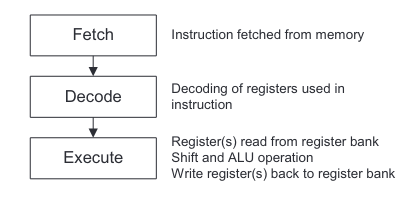
\includegraphics[width=.5\textwidth]{capitulos/capitulo2/pipeline.png}
		    \caption{Segmentación de instrucciones de la Game Boy Advance.}
		    \label{fig:pipeline}
		\end{figure}

	\item Una ALU de 32 bits, mejorando de forma sustancial las capacidades de modelos anteriores. De esta forma, la consola podía operar con números de 32 bits sin tener que consumir ciclos adicionales del procesador.
	\item Un procesador con extensiones específicas, las cuales aparecen en el propio nombre, ARM7\textbf{TDMI}. A continuación se detallan:

		\begin{itemize}
			\item \underline{\textbf{T}}humb: Tal y como se indicó previamente, el procesador soporta un modo que opera con instrucciones de 16 bits. Al ejecutarse en el hardware, las instrucciones se descomprimen a instrucciones de 32 bits sin pérdida de rendimiento. Según las estimaciones de ARM, programar en el modo THUMB reduce el tamaño del programa un 35\% (comparado con el modo ARM) y proporciona un rendimiento del 160\% al utilizarse en sistemas que trabajan en 16 bits \cite{bib:arm}. Todas las mejoras mencionadas anteriormente son posibles siempre y cuando las limitaciones que implica el modo (el limitado acceso a los registros superiores, R8-R12, por ejemplo) no supongan un inconveniente al programar.
			\item Extensiones de \underline{\textbf{D}}epuración mediante JTAG: \textit{Joint Test Access Group} o \textit{Standard Test Access Port and Boundary-Scan Architecture}, siendo este último el nombre oficial dado por la IEEE. Se trata de una especificación que permite a partir de una conexión, depurar un microcontrolador directamente en el hardware.
		\item \underline{\textbf{M}}ultiplicador mejorado: Los ciclos necesarios para completar multiplicaciones con números de 32 bits se reducen de forma considerable con respecto a las versiones anteriores del procesador.
		\item Embedded\underline{\textbf{I}}CE macrocell: Con ICE, \textit{In-circuit emulation} en inglés, la consola añade la posibilidad de manipular directamente el hardware del dispositivo para poder realizar una depuración a fondo del programa.
		\end{itemize}

		La distribución de la lógica necesaria para poder incluir las extensiones de depuración mediante JTAG y EmbeddedICE macrocell se puede observar en la Figura~\ref{fig:debug_block}. Aquí se puede ver también la adición de un controlador llamado ``TAP''. Este sirve de intermediario entre la interfaz serial JTAG y las \textit{scan chains}, que habilitan la comunicación entre la interfaz ICE y el procesador de la consola.

		\begin{figure}[h]
		    \centering
		    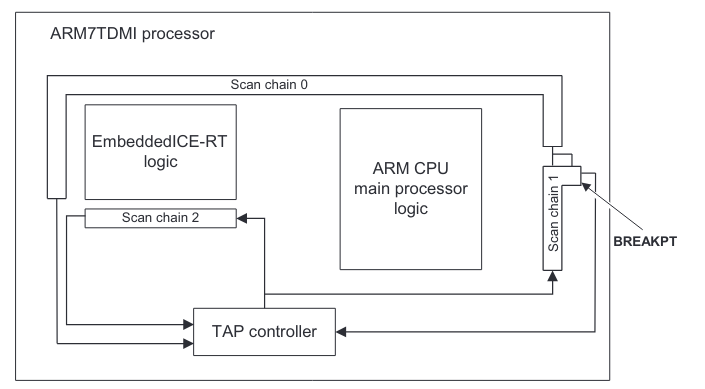
\includegraphics[width=.8\textwidth]{capitulos/capitulo2/debug_block.png}
		    \caption{Distribución del EmbeddedICE-RT y controlador TAP en el diagrama de bloques del ARM7TDMI.}
		    \label{fig:debug_block}
		\end{figure}
		\FloatBarrier{}

\end{enumerate}

El lector interesado puede consultar \cite{bib:arm} para obtener más información sobre el procesador ARM7TDMI.

\section{Coprocesador Sharp SM83}
Para mantener la retrocompatibilidad de modelos anteriores con la Game Boy Advance, Nintendo incluyó un coprocesador que se encargaría de llevar a cabo esta labor. Como era de esperar, la compañía incluyó el mismo procesador utilizado para la Game Boy original, un procesador Sharp SM83 dentro del SoC Sharp LR35902. El procesador, dependiendo del dispositivo, funcionaba a una frecuencia de 4.19 MHz u 8.38 MHz. Por aquel entonces, incluir el hardware de dispositivos anteriores era una práctica convencional, puesto que el hardware no era lo suficientemente potente como para emular generaciones pasadas. La situación hoy en día es diferente según el caso. Por ejemplo, la Xbox One ya incluye un emulador para poder ejecutar juegos de Xbox 360\footnote{https://www.extremetech.com/gaming/257851-microsoft-built-xbox-360-xbox-compatibility-xbox-one}. 

La información disponible sobre el procesador Sharp es escasa. No obstante, se sabe que su diseño se basa, fundamentalmente, en los procesadores \textbf{Intel 8080} y \textbf{Zilog Z80}. A continuación se detallarán las características heredadas de cada uno de ellos.

La primera característica, que se hace evidente al saber en los dos procesadores en los que se basa, es que el \textbf{Sharp SM83 es un procesador de 8 bits}.

Sharp, al diseñar el procesador, combinó características de cada uno. Una de ellas sería la sintaxis utilizada al programar en ensamblador, en concreto, la sintaxis utilizada por el Z80. Esta se escogería seguramente por el \textit{copyright} que tenía Intel en su día sobre la sintaxis utilizada en el 8080. Por lo tanto, las diferencias encontradas son menores. Los únicos cambios son el de los nombres de instrucciones abreviadas que utilizaba Intel, que se reemplazaron por otras que usaban el nombre completo (por ejemplo, ``LOAD'' en vez de ``LD'').

En cuanto a registros se refiere, se tomó prestado el diseño utilizado en el Intel 8080, pero con ligeras modificaciones que destacaremos a continuación. En concreto, los \textbf{10 registros} que utiliza el procesador Sharp son:

\begin{itemize}
\item El registro A de 8 bits, reservado para el acumulador.
\item El registro F de 8 bits, reservado para guardar el estado del procesador.
\item El resto de registros (el B, C, D, E, H, y L) de 8 bits, diseñados para un uso general por parte del programador.
\item Los registros PC y SP, de 16 bits cada uno, se reservaban para su uso como contador de programa y puntero de pila, respectivamente.
\end{itemize}

Dado que algunas instrucciones lo permitían, se podían utilizar los registros en pares de la siguiente manera: AF, BC, DE y HL.

A pesar de tomar prestado el diseño de los registros, lo que \textbf{no heredó fue el esquema I/O del Intel 8080}, que permitía acceder a cada puerto mediante una instrucción específica. Se optó por el mismo sistema que utiliza la Game Boy Advance, ``mapeando'' cualquier puerto a una zona de memoria.

Otra especificación que copió del Intel 8080 fue el \textbf{bus de datos de 8 bits y direccionamiento de 16 bits}, con el cual se podían acceder a 64 KB de memoria.

\section{El registro I/O}

La Game Boy Advance ``mapea'' los registros I/O de control directamente en memoria, utilizando parte del espacio de memoria disponible para el dispositivo. A pesar de disminuir el espacio de memoria disponible, Nintendo consigue de esta forma reducir costes y simplificar el diseño interno comparado con la alternativa, un diseño I/O independiente.

En este punto se incluyen las principales regiones utilizadas para configurar las funciones comentadas en el informe y requeridas en el código del proyecto (véase el Capítulo~\ref{sec:desarrollo}). Todos los registros, incluyendo los no mencionados en esta sección, se podrán consultar en el Apéndice~\ref{ap:registros}, en el que se describe brevemente cada uno junto con su nombre y tamaño. Toda la información del apéndice ha sido extraída de~\cite{bib:gbatek}.

El mapa I/O de la consola está conformado por 7 secciones: Los \textbf{registros LCD}, \textbf{registros de sonido}, \textbf{canales DMA}, \textbf{registros de temporización}, \textbf{comunicación serie}, \textbf{botones del dispositivo} y \textbf{control de interrupciones}~\cite{bib:gbatek}. En los siguientes puntos se describirán cada una de ellas. Es importante mencionar que la extensión de cada uno de los puntos será proporcional a la importancia que tenga esa sección en particular para el proyecto. Toda la información mostrada en este punto, al tener una naturaleza puramente técnica con las especificaciones de Nintendo, tendrá como base~\cite{bib:gba_manual} y~\cite{bib:gbatek} .

\subsection{Registros LCD}\label{sec:dispcnt}
En los registros LCD se incluyen todos los parámetros utilizados para configurar la imagen que se muestra por pantalla.

\subsubsection{DISPCNT}
El primer registro que se encuentra en esta región es el denominado \textit{Display Control} (o como se referencia en~\cite{bib:gbatek}, DISPCNT), situado en la dirección de memoria 0x04000000. Entre los parámetros que se pueden modificar se encuentran:

\begin{itemize}
	\item Bit \{F\}: El modo ``ventana'' reservado para sprites.
	\item Bits \{E-D\}: Los bits para activar los dos modos ``ventana'' reservados para los 4 fondos diferentes.
	\item Bit \{C\}: Activa el uso de sprites.
	\item Bits \{B-8\}: Cada uno de los bits en este rango activa los 4 fondos que puede tener la GBA en un momento dado. Los bits \{B-8\} activan los fondos 3, 2, 1 y 0 respectivamente.
	\item Bit \{7\}: Provoca un ``reset'' de la pantalla para que se muestre una imagen completamente blanca ignorando cualquier contenido almacenado en la VRAM y OAM\@.
	\item Bit \{6\}: Especifica la manera en la que están distribuidos los tiles en la OAM\@. Para 0, la distribución será de dos dimensiones mientras que para 1, la distribución será unidimensional. Véase la Figura~\ref{fig:1d} para una configuración 1D de los \textit{tiles} en memoria y la Figura~\ref{fig:2d} para observar una configuración 2D de los \textit{tiles}.

		\begin{figure}[h]
			\centering
			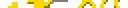
\includegraphics[width=.7\textwidth]{capitulos/capitulo4/new_1d.png}
			\caption{Distribución 1D de los \textit{tiles} en la OAM.}\label{fig:1d}
		\end{figure}

		\begin{figure}[h]
			\centering
			
\includegraphics[width=.4\textwidth]{capitulos/capitulo4/new_2d.png}
			\caption{Distribución 2D de los \textit{tiles} en la OAM.}\label{fig:2d}
		\end{figure}

	\item Bit \{5\}: Al activar este bit, el programador tendrá acceso a la OAM durante HBlank.
	\item Bit \{4\}: Permite la selección del buffer que se muestra por pantalla para los modos 4 y 5, los cuales manejan más de un buffer. Para más información consultar el punto~\ref{sec:mode_4} y~\ref{sec:mode_5}. 
	\item Bit \{3\}: La función que desempeña el tercer bit del registro DISPCNT es mostrar si el juego se está ejecutando en una Game Boy Color. El bit no se puede modificar. 
	\item Bits \{2-0\}: Modo del fondo utilizado. Entre los valores permitidos están el 0, 1 y 2, definidos para las tres maneras que tiene la GBA de procesar fondos. Los modos 3, 4 y 5 están reservados para los fondos bitmap. Los valores 6 y 7 no están permitidos. Las diferencias entre los modos se verán en las secciones~\ref{sec:bitmaps} y~\ref{sec:fondos}.
\end{itemize}

En la Tabla~\ref{tab:dispcnt} se hace un resumen de los parámetros del registro DISPCNT.

\begin{table}[h]
	\centering
	\begin{tabular}{| l | l |}
		\hline
		\textbf{Bits} & \textbf{Función}  \\ \hline
		F & Modo ``ventana'' para \textit{sprites}.  \\ \hline
		E-D & Modo ``ventana'' para fondos.  \\ \hline
		C & Activa el uso de \textit{sprites}.  \\ \hline
		B-8 & Activa cada uno de los 4 fondos disponibles.  \\ \hline
		7 & ``Reset'' de la pantalla.  \\ \hline
		6 & Especifica la distribución de los tiles en memoria. \\ \hline
		5 & Activa el acceso a la OAM durante HBlank. \\ \hline
		4 & Selecciona el buffer adicional en los modos 4 y 5. \\ \hline
		3 & Permite consultar si un juego se está ejecutando en una Game Boy Color. \\ \hline
		2-0 & Selecciona el modo que utiliza la Game Boy Advance para los fondos. \\ \hline
	\end{tabular}
	\caption{Registro \textit{Display Control}.}\label{tab:dispcnt}
\end{table}
\FloatBarrier{}

\subsubsection{DISPSTAT}

El siguiente registro, el \textit{Display Status} (conocido también como el registro DISPSTAT), se sitúa en la dirección de memoria 0x04000004 y permite al programador consultar la información relacionada con el VBlank, HBlank y VCount. VBlank es el período que hay entre cada fotograma refrescado, y HBlank se refiere al período que hay entre cada línea refrescada por pantalla. Por otro lado, VCount es el número de líneas, las filas de píxeles horizontales, refrescadas. Los bits que contiene son los siguientes:
\begin{itemize}
	\item Bits \{F-8\}: El programador especifica un valor VCount determinado, para invocar una interrupción en el bit {5} o que el cambio se vea reflejado en el bit {2}.
	\item Bit \{5\}: Activa la interrupción de VCount si este coincide con el valor especificado en {F-8}.
	\item Bits \{4-3\}: Activa la interrupción de HBlank y VBlank respectivamente.
	\item Bit \{2\}: Este bit tendrá valor si VCount coincide con el valor especificado en {F-8}.
	\item Bits \{1-0\}: Permiten saber si el dispositivo se encuentra en HBlank, si el valor del bit 0 es 1, o en VBlank, si el valor del bit 1 es 1.
\end{itemize}

En la Tabla~\ref{tab:dispstat} se hace un resumen de los parámetros del registro DISPSTAT.

\begin{table}[h]
	\centering
	\begin{tabular}{| l | l |}
		\hline
		\textbf{Bits} & \textbf{Función}  \\ \hline
		F-8 & VCount objetivo.  \\ \hline
		5 & Activa una interrupción al alcanzar VCount objetivo. \\ \hline
		4-3 & Activa la interrupción de HBlank y VBlank. \\ \hline
		2 & Bit activo en caso de alcanzar VCount objetivo.  \\ \hline
		1-0 & Esto de HBlank y VBlank. \\ \hline
	\end{tabular}
	\caption{Registro \textit{Display Status}.}\label{tab:dispstat}
\end{table}
\FloatBarrier{}

El valor de VCount también se puede consultar en la dirección de memoria 0x04000006. Dado que el valor oscila entre 0 y 227, solo se tienen en cuenta los primeros 8 bits.

\subsubsection{Configuración de fondos}\label{sec:conf_fondos}

A continuación, se detallan los registros para controlar los distintos parámetros que pueden tener los fondos de la Game Boy Advance. Estos registros sirven, entre otras cosas, para cambiar el tamaño, color y posicionamiento de los fondos.

\begin{itemize}
	\item Bits \{F-E\}: Tamaño del fondo. Para más información consultar la sección~\ref{sec:fondos}.
	\item Bit {D}: Por defecto, los fondos que no utilizan la matriz de transformación, se repiten en caso de que el \textit{offset} provoque que el fondo llegue a su fin. Este campo permite que los fondos que utilicen la matriz de transformación también se vean repetidos. Para más información, consultar el punto~\ref{sec:fondos}.
	\item Bits \{C-8\}: El índice del grupo de \textit{tiles} especifico que se utiliza.
	\item Bit {7}: Especifica el formato del color a utilizar. Con un 0 se consiguen 16 colores disponibles (4 bpp) y con un 1 se consiguen 256 colores (8 bpp).
	\item Bit {6}: Activa el modo mosaico. Más información en el punto~\ref{sec:sprites}.
	\item Bits \{3-2\}: Especifica el índice del bloque de grupo de \textit{tiles} a utilizar.
	\item Bits \{1-0\}: Prioridad de renderizado del fondo. Cuánto mayor sea el valor antes se renderizará en pantalla. En caso de que haya fondos con la misma prioridad se recurre al orden natural, siendo el primer fondo (BG0) el que mayor prioridad tiene y el último fondo el que menor prioridad tiene (BG3).
\end{itemize}

En la Tabla~\ref{tab:regfondo} se hace un resumen de los parámetros del registro de control de fondos.

\begin{table}[h]
	\centering
	\begin{tabular}{| l | l |}
		\hline
		\textbf{Bits} & \textbf{Función}  \\ \hline
		D & Activar la función ``wrap'' en las matrices que utilicen la matriz de transformación. \\ \hline
		C-8 & El índice del grupo de \textit{tiles} especifico que se utilizará.   \\ \hline
		7 & Rango de colores utilizado.  \\ \hline
		6 & Modo mosaico.  \\ \hline
		3-2 & Especifica el índice del bloque de grupo de \textit{tiles} que se utilizará. \\ \hline
		1-0 & Prioridad de renderizado. \\ \hline
	\end{tabular}
	\caption{Registro de control de fondos.}\label{tab:regfondo}
\end{table}
\FloatBarrier{}

Cada uno de los fondos cuenta con un registro de control específico. La ubicación de los registros para cada fondo se puede observar en la Tabla~\ref{tab:fondo_reg_1}. Además, en la tabla se incluye el \textit{offset} X e Y mencionado anteriormente.

En caso de que el programador quiera renderizar los fondos a través de una matriz de transformación dada (más información en el punto~\ref{sec:ppu}), tiene que configurar los registros de transformación y los registros de referencia. Este último sustituye a los parámetros de \textit{offset} vistos anteriormente para los fondos ``normales'' (aquellos que no utilicen la matriz de transformación).

\begin{table}[h]
	\centering
	\begin{tabular}{| l | l | l | l | l |}
		\hline
		\textbf{Fondos} & \textbf{Registro de Control} & \textbf{Registro de Offset X} & \textbf{Registro de Offset Y}  \\ \hline
		0 & 0x04000008 & 0x04000010 & 0x04000012  \\ \hline
		1 & 0x0400000A & 0x04000014 & 0x04000016  \\ \hline
		2 & 0x0400000C & 0x04000018 & 0x0400001A  \\ \hline
		3 & 0x0400000E & 0x0400001C & 0x0400001E  \\ \hline
	\end{tabular}
	\caption{Registros de cada uno de los fondos (1).}\label{tab:fondo_reg_1}
\end{table}
\FloatBarrier{}

El registro de transformación, como su nombre indica, se limita a almacenar los valores de la matriz de transformación. Los valores de la matriz 2x2 se almacenan consecutivamente, ocupando 2 bytes cada uno, empezando por 0x04000020 para el fondo 2 y 0x04000030 para el fondo 3 (véase la Tabla~\ref{tab:fondo_reg_2}). Estos valores son números \textit{fixed point} desplazados por 8 bits.

\begin{table}[h]
	\centering
	\begin{tabular}{| l | l | l | l | l |}
		\hline
		\textbf{Fondos} & \textbf{Registro de Transformación} & \textbf{Registro de Referencia}  \\ \hline
		0 &  - & -  \\ \hline
		1 & - & -  \\ \hline
		2 & 0x04000028-0x0400002E & 0x04000020-0x04000026  \\ \hline
		3 & 0x04000038-0x0400003E & 0x04000030-0x04000036  \\ \hline
	\end{tabular}
	\caption{Registros de cada uno de los fondos (2).}\label{tab:fondo_reg_2}
\end{table}

El otro registro a tener en cuenta, es el registro de referencia. Este replica el comportamiento del registro de \textit{offset} pero con números \textit{fixed point} de 28 bits. La distribución de los valores es la mostrada en la Tabla~\ref{tab:dist_fixed_fondo}.

\begin{table}[h]
	\centering
	\begin{tabular}{| l | l | l |}
		\hline
		27 & 26--8 & 7--0  \\ \hline
		Signo & Valor entero & Valor decimal  \\ \hline
	\end{tabular}
	\caption{Formato del valor de referencia de los fondos utilizando la matriz de transformación.}\label{tab:dist_fixed_fondo}
\end{table}

Los puntos de referencia X e Y para el fondo 2 se almacenan en las direcciones de memoria 0x04000028 y 0x0400002E respectivamente, mientras que los puntos de referencia X e Y para el fondo 3 se localizan en las direcciones de memoria 0x04000038 y 0x0400003E respectivamente (véase la Tabla~\ref{tab:fondo_reg_2}).

Como se puede apreciar en la Tabla~\ref{tab:fondo_reg_2}, los fondos 0 y 1 no cuentan con la posibilidad de poder utilizar la matriz de transformación.

\subsubsection{Registros de efectos especiales}

Finalmente, en la sección de registros LCD, las tres secciones que quedan son las del modo ventana, modo mosaico y otros efectos especiales. Las demostraciones de estas tres funciones se pueden ver en la Sección~\ref{sec:efectos}.

Dado que se pueden crear dos ventanas diferentes, existen dos registros distintos para cada uno, donde se especifican las dimensiones horizontales y verticales del rectángulo creado. Las dimensiones horizontales se indican en las direcciones 0x04000040 y 0x04000042 para las ventanas 0 y 1 respectivamente. De los 2 bytes que conforman cada valor, se utiliza 1 byte para cada una de las dos coordenadas X que representan las esquinas inferior izquierda y superior derecha del rectángulo. El formato para las coordenadas verticales es exactamente el mismo pero en las direcciones 0x04000044 para la ventana 0 y 0x04000046 para la ventana 1. En caso de que los valores superen la resolución del dispositivo (240x160), el valor introducido se interpreta como el máximo permitido. En el caso de la anchura, 240, y en el caso de la altura, 160. 

Sin embargo, antes de poder configurar las posiciones de las ventanas es necesario especificar cómo funcionan. Para ello se tiene que definir el comportamiento dentro de la ventanas, en el registro WININ en la dirección de memoria 0x04000048, y el comportamiento fuera de estas, en el registro WINOUT en la dirección de memoria 0x0400004A. Los parámetros para WININ son:

\begin{itemize}
	\item Bit \{D\}: Activa efectos especiales como el \textit{blending} y los efectos \textit{fade in} y \textit{fade out} para la ventana 1.
	\item Bit \{C\}: Activa el renderizado de \textit{sprites} para la ventana 1.
	\item Bits \{B-8\}: Activa los fondos 3, 2, 1 y 0, respectivamente, para la ventana 1.
	\item Bit \{5\}: Activa efectos especiales como el \textit{blending} y los efectos \textit{fade in} y \textit{fade out} para la ventana 0.
	\item Bit \{4\}: Activa el renderizado de \textit{sprites} para la ventana 0.
	\item Bits \{3-0\}: Activa los fondos 3, 2, 1 y 0, respectivamente, para la ventana 0.
\end{itemize}

Por otro lado, para controlar lo que se renderizá fuera de la ventana se configuran los siguientes parámetros en WINOUT:

\begin{itemize}
	\item Bit \{D\}: Activa efectos especiales fuera de las ventanas de \textit{sprites}.
	\item Bit \{C\}: Activa el renderizado de \textit{sprites} fuera de una ventana de \textit{sprites}.
	\item Bits \{B-8\}: Activa el renderizado de los fondos 3, 2, 1 y 0, respectivamente, fuera de una ventana de \textit{sprites}.
	\item Bit \{5\}: Activa efectos especiales fuera de las ventana de las de fondo.
	\item Bit \{4\}: Activa el renderizado de \textit{sprites} fuera de una ventana de fondo.
	\item Bits \{3-0\}: Activa el renderizado de los fondos 3, 2, 1 y 0, respectivamente, fuera de las ventanas de fondo.
\end{itemize}

El registro para la función mosaico se encuentra en la dirección de memoria 0x0400004C. El efecto distorsiona (o ``pixela'') la imagen dependiendo del valor que especifique el programador. Para una demostración del efecto consultar la Sección~\ref{sec:efectos}. Los bits que contiene son los siguientes:

\begin{itemize}
	\item Bits \{F-C\}: Distorsión en el eje vertical del \textit{sprite}.
	\item Bits \{B-8\}: Distorsión en el eje horizontal del \textit{sprite}.
	\item Bits \{7-4\}: Distorsión en el eje vertical del fondo.
	\item Bits \{3-0\}: Distorsión en el eje horizontal del fondo.
\end{itemize}

La última región de los registros LCD son aquellos dedicados al renderizado de efectos especiales. En concreto, los que permiten la mezcla de colores (o transparencia) y cambio de intensidad en la representación de los colores\footnote{Un incremento en la intensidad se traduce en una imagen más ``blanca'' mientras que una imagen con menos intensidad se traduce en una imagen más oscura.}.

El principal registro que gestiona toda la configuración relacionada con los efectos especiales es el registro posicionado en 0x04000050, denominado en~\cite{bib:gbatek} como BLDCNT. Los bits que contiene son los siguientes: 

\begin{itemize}
	\item Bits \{D-8\}: Selección de las capas posteriores a mezclar. Cada bit activa el ``backdrop''\footnote{El ``backdrop'' de la GBA consiste en un fondo completamente negro.}, \textit{sprites} y fondos 3, 2, 1 y 0, respectivamente.
	\item Bits \{7-6\}: Selección del efecto a procesar. Siendo 3, se traduce en un incremento en la intensidad de la capa frontal. Si es 2, se hace una disminución en la intensidad de la capa frontal Cuando es 1, se hace una mezcla de colores de las capas frontales con las posteriores seleccionadas. Finalmente, el 0 significa que no se escoge ningún efecto. Para que la mezcla de colores funcione como se espera es necesario que la capa frontal se encuentre, como su nombre indica, por encima de la capa (o capas) posteriores. 
	\item Bits \{5-0\}: Selección de las capas frontales a mezclar. Cada bit activa el ``backdrop'', \textit{sprites} y fondos 3, 2, 1 y 0, respectivamente.
\end{itemize}

Para poder procesar los efectos tal y como desea el programador, este tiene que especificar los valores adecuados en los registros BLDALPHA para configurar el nivel de mezcla entre las capas frontales y posteriores, en 0x0400052. De forma adicional, para controlar el nivel de intensidad en las capas seleccionadas, tendrá que modificar el valor de BLDY en 0x04000054.

En el caso del registro BLDALPHA, que ocupa 2 bytes, los bits \{C-8\} denotan el coeficiente que tendrán las capas posteriores mientras que los bits \{4-0\} indican el coeficiente que tendrán las capas frontales. De forma similar a lo que ocurre con los registros de los fondos que utilizan las matrices de transformación, los 4 bits inferiores de cada coeficiente simbolizan incrementos fraccionales de $1/16$, teniendo cada coeficiente un rango entre 0 y 1. En el caso del registro BLDY, ocurre lo mismo pero solo utilizando los bits \{4-0\} para especificar un valor entre 0 y 1.

\subsection{Registros de sonido}

La Game Boy Advance ofrece 6 modos diferentes de sonido, 4 analógicos y 2 digitales (canales A-B). Hay un registro para controlar cada uno de ellos además de varios generales que controlan el volumen.

El término técnico para referirse a las 6 opciones de la consola para ofrecer audio es ``canal''. Sin embargo, para no confundirlo con los canales de izquierda y derecha, a lo largo del trabajo, se hará referencia a los 6 canales como ``modos''.

La información contenida en esta sección se basa en la documentación oficial~\cite{bib:gba_manual} y en el material adicional disponible en~\cite{bib:belogic}.

\subsubsection{Modos analógicos}
Los dos primeros modos que ofrece el hardware de la consola, los canales 1 y 2, permiten la reproducción de pulsos con la posibilidad de modificar el volumen de cada onda. De forma adicional, el primer modo permite cambiar de dinámicamente la frecuencia de las ondas. Para ello, ambos modos harán uso de registros para modificar el tono y la duración de la onda, teniendo el modo 1 un registro adicional para controlar la frecuencia. 

El registro encargado de la duración, volumen y ciclo de la onda utiliza el siguiente formato para los modos 1 y 2:

\begin{itemize}
	\item Bits \{F-C\}: Volumen inicial del sonido.
	\item Bit \{B\}: Modificación del volumen. 0 para disminuirlo conforme pasa el tiempo y 1 para incrementarlo conforme pasa el tiempo. 
	\item Bits \{A-8\}: El período con el que cambia el volumen. El valor especificado resulta en $n/64$ segundos de período. 
	\item Bits \{7-6\}: El ciclo que toma el pulso. 0 para un ciclo del 12.5\%, 1 para un ciclo del 25\%, 2 para un ciclo del 50\% y 3 para un ciclo del 75\%.
	\item Bits \{5-0\}: La duración del sonido. El valor especificado resulta en $(64-n)/256$ segundos.
\end{itemize}

El registro encargado de la frecuencia de la onda utiliza el siguiente formato para los modos 1 y 2:

\begin{itemize}
	\item Bit \{F\}: En caso de estar activo el bit, ``resetea'' el sonido.
	\item Bit \{E\}: En caso de ser 0, el sonido es reproducido de forma constante. Si es 1, el sonido es reproducido con la duración especificada en los bits \{5-0\} del registro anterior.
	\item Bits \{A-0\}: Frecuencia utilizada para el tono. El valor especificado resulta en $131072/(2048-n)$ Hz.
\end{itemize}

Para indicar un cambio dinámico en la frecuencia, el modo 1 cuenta con el registro ``sweep'', que tiene los siguientes bits:

\begin{itemize}
	\item Bits \{6-4\}: El tiempo que pasa entre cambios de frecuencia. El valor especificado resulta en $n/128$ segundos.
	\item Bit \{3\}: Cómo se modifica la frecuencia. 0 para el incremento con el paso del tiempo y 1 para la disminución.
	\item Bits \{2-0\}: Denota el cambio en la frecuencia. El valor especificado resulta en un cambio en el periodo de $T=T\pm{}T/2^n$. La suma o resta dependerá del valor del bit {3}.
\end{itemize}

En la Tabla~\ref{tab:reg_canal_1_2} se incluyen los registros de los modos 1 y 2.

\begin{table}[h]
	\centering
	\begin{tabular}{| l | l | l | l |}
		\hline
		\textbf{Canal} & \textbf{Registro de duración} & \textbf{Registro de frecuencia} & \textbf{Registro ``sweep''} \\ \hline
		1 & 0x04000062 & 0x04000064 & 0x04000060 \\ \hline
		2 & 0x04000068 & 0x0400006C & - \\ \hline
	\end{tabular}
	\caption{Registros dedicados de los modos 1 y 2.}\label{tab:reg_canal_1_2}
\end{table}
\FloatBarrier{}

El modo 3, permite reproducir ondas almacenadas en el espacio de memoria localizado entre 0x04000090 y 0x0400009F. En este modo se pueden diferenciar los registros de control para la selección, duración y frecuencia.

El primer registro, reservado para seleccionar la muestra localizada en [0x04000090, 0x0400009F] y utilizado para activar el modo, tiene el siguiente formato:

\begin{itemize}
	\item Bit \{7\}: Activa el modo.
	\item Bit \{6\}: Selecciona el grupo a utilizar. Complementa al bit {5}.
	\item Bit \{5\}: En caso de que el valor sea 0, la Game Boy Advance dividirá las ondas almacenadas en el rango de memoria especificado anteriormente en dos grupos diferentes de 32 muestras cada una. En caso de ser 1, gestionará toda la información almacenada en el rango como un solo grupo de 64 muestras.
\end{itemize}

El segundo registro, es el encargado de modificar la duración y el volumen del modo 3:

\begin{itemize}
	\item Bits \{F-D\}: Volumen del modo. 0 para 0\%, 1 para 100\%, 4 para 75\%, 2 para 50\% y 3 para el 25\%.
	\item Bits \{7-0\}: La duración del sonido. El valor especificado resulta en $n/256$ segundos.
\end{itemize}

Finalmente, el tercer registro necesario para utilizar el modo 3 es el encargado de configurar la frecuencia y repetición del sonido. Tiene el mismo formato descrito para los modos 1 y 2, y cuenta con los siguientes bits:

\begin{itemize}
	\item Bit \{F\}: En caso de estar activo el bit, ``resetea'' el sonido.
	\item Bit \{E\}: Si es 0, reproduce el sonido de forma constante. Si es 1, reproduce el sonido con la duración especificada en los bits \{5-0\} del registro anterior.
	\item Bits \{A-0\}: Frecuencia utilizada para el tono. El valor especificado resulta en $131072/(2048-n)$ Hz.
\end{itemize}

El último modo analógico, el modo 4, tiene como función generar ruido como añadido a los demás modos. De los dos registros reservados para el modo, el que controla la duración y el volumen sigue el mismo formato presentado anteriormente. El registro diferente que se introduce en este caso, es el registro de ruido, que tiene la siguiente estructura:

\begin{itemize}
	\item Bit \{F\}: En caso de estar activo el bit, ``resetea'' el sonido.
	\item Bit \{E\}: Si es 0, reproduce el sonido de forma constante. Si es 1, reproduce el sonido con la duración especificada en los bits \{5-0\} del registro anterior.
	\item Bits \{7-4\}: Denota la función a utilizar con la frecuencia especificada en los bits \{2-0\}. La salida de la función (o \textit{pre-scaler divider} como se llama en~\cite{bib:belogic}) será utilizada para generar el ruido. El efecto del valor del campo sobre la función se puede observar en la ecuación~\ref{eq:fn_canal_4}.

	\begin{align}
		Q/2^{valor+1}
		\label{eq:fn_canal_4}
	\end{align}

	\item Bit \{3\}: Controla el período del ruido generado. Si es 0, el periodo es de 127 ciclos y si es de 1, el periodo es de 32767 ciclos.
	\item Bits \{2-0\}: Frecuencia utilizada en conjunto con la función denotada en [7-4] para generar ruido. Las frecuencias vinculadas a los 8 valores disponibles se pueden observar en la Tabla~\ref{tab:frec_canal_4}.

	\begin{table}[h]
		\centering
		\begin{tabular}{| l | l |}
			\hline
			\textbf{Valor} & \textbf{Frecuencia (en MHz)}  \\ \hline
			0 & $4.19304/2$ \\ \hline
			1 & $4.19304/8$ \\ \hline
			2 & $4.19304/16$ \\ \hline
			3 & $4.19304/24$ \\ \hline
			4 & $4.19304/32$ \\ \hline
			5 & $4.19304/40$ \\ \hline
			6 & $4.19304/48$ \\ \hline
			7 & $4.19304/56$ \\ \hline
		\end{tabular}
		\caption{Frecuencias disponibles para generar ruido en el modo 4.}\label{tab:frec_canal_4}
	\end{table}
	\FloatBarrier{}
\end{itemize}

\subsubsection{Modos digitales}
Se introdujeron dos nuevos modos con respecto al sistema de audio de la Game Boy Color. Estos modos, denominados A y B, hacen uso de los dos DACs (Conversor Digital Analógico) de 8 bits incorporados en la consola. Para utilizarlos se distinguen dos tipos de registros, aquellos reservados para indicar los datos a usar y otros para configurar los modos, los registros de control.

Los registros de datos de los modos A y B, se encuentran en las regiones 0x040000A0 y 0x040000A4, respectivamente. El sistema que implementa la Game Boy Advance, denominado Direct Sound, coge los primeros datos que encuentra en el buffer (FIFO), es decir, los 8 bits menos significativos del registro de 32 bits, que serán los primeros en reproducirse. Para activar la salida de sonido de estos modos, y también los modos 1-4, se utilizan tres registros de control. El primero está en 0x04000080 y tiene como función activar y controlar de forma global el volumen de los modos 1-4. Tiene el siguiente formato:

\begin{itemize}
	\item Bits \{F-C\}: Cada uno de los 4 bits activa el canal izquierdo para los modos 1-4.
	\item Bits \{B-8\}: Cada uno de los 4 bits activa el canal derecho para los modos 1-4.
	\item Bits \{6-4\}: Volumen en el canal izquierdo de los primeros 4 modos.
	\item Bits \{2-0\}: Volumen en el canal derecho de los primeros 4 modos.  
\end{itemize}

El segundo registro de control utilizado es el posicionado en la dirección de memoria 0x04000082. Este modifica el volumen global de los modos 1-4 para los dos canales, además de configurar parámetros relacionados con los modos A y B. Tiene el siguiente formato:

\begin{itemize}
	\item Bit \{F\}: Restablece el buffer de datos FIFO del modo B.
	\item Bit \{E\}: Para poder reproducir sonido en los modos A y B, es necesario utilizar el temporizador 0 o 1. En este campo se especifica cual de los dos temporizadores se utilizará para el modo B.
	\item Bits \{D-C\}: Activa los canales izquierdo (2) y/o derecho (1) del modo B.
	\item Bit \{B\}: Restablece el buffer de datos FIFO del modo A.
	\item Bit \{A\}: Al igual que en el campo {E} se especifica el temporizador a utilizar para el modo A, número 0 o 1.
	\item Bits \{9-8\}: Activa los canales izquierdo (2) y/o derecho (1) del modo A.  
	\item Bit \{3\}: Volumen global del modo B.  
	\item Bit \{2\}: Volumen global del modo A.  
	\item Bits \{1-0\}: Volumen global de los primeros 4 modos. 
\end{itemize}

Finalmente, el registro denominado el ``master switch'' se posiciona en la dirección de memoria 0x04000084. El registro también puede servir para consultar el estado actual en el que se encuentran los modos 1-4. Es importante mencionar que los bits destinados a consultar el estado actual de un modo no pueden ser sobrescritos por el programador.

\begin{itemize}
	\item Bit \{7\}: Permite desactivar todos los modos que ofrece la Game Boy Advance al igualar el campo a 0.
	\item Bits \{3-0\}: Especifica el estado de los modos 4, 3, 2 y 1, respectivamente. Un valor igual a 1 denota que el estado está activo, mientras que el 0 indica lo contrario.
\end{itemize}

\subsection{Registros para \textit{Direct Memory Access}}
La GBA ofrece la posibilidad de copiar datos rápidamente de una dirección de memoria a otra mediante el uso de \textit{Direct Memory Access} (DMA)~\cite{bib:dma_book}.

La consola cuenta con 4 variantes de \textit{DMA} con diferentes prioridades y, por ende, finalidades. El canal número 0 permite realizar transferencias con la máxima prioridad disponible. Los canales 1 y 2 se reservan para las transferencias de sonido a los buffers adecuados. Por último, el canal 3 se reserva para transferencias generales.

Los registros de 32 bits que permiten llevar a cabo estas operaciones son los registros fuente, destino y de control \textit{DMA}. Estos tres registros se repiten para cada uno de los 4 canales. En concreto, el registro de control \textit{DMA} sigue el formato descrito a continuación:

\begin{itemize}
	\item Bit \{1F\}: Activa una transferencia mediante \textit{DMA}.
	\item Bit \{1E\}: Activa una interrupción en caso de haberse completado la operación. 
	\item Bits \{1D-1C\}: Especifica cuándo debe comenzar la transferencia: 0 de manera inmediata, 1 al entrar en el estado VBlank, 2 al entrar en el estado HBlank y el comportamiento al igualar a 3 dependerá del canal utilizado. Para los canales reservados para audio se empieza la transferencia una vez que se hayan leído los buffers correspondientes. Para el canal 3 se realiza una transferencia antes de que la \textit{PPU} renderice cada línea horizontal de la pantalla~\cite{bib:tonc}.
	\item Bit \{1A\}: Especifica el tamaño del dato a copiar. 0 para 16 bits y 1 para 32 bits. 
	\item Bit \{19\}: Si se ha seleccionado el modo 1 en los bits \{1D-1C\}, se repite la transferencia cada vez que el dispositivo entre en el estado VBlank. En el caso de haber seleccionado el modo 2 en los bits \{1D-1C\}, se repite la transferencia cada vez que el dispositivo entre en el estado HBlank.
	\item Bits \{18-17\}: Definen la modificación de la dirección fuente que se lleva a cabo al completar una copia: 0 para incrementar la dirección fuente, 1 para decrementar la dirección fuente, 2 para dejar la dirección de destino fija y 3 para incrementar la dirección fuente, restableciendo el valor inicial una vez acabada la operación. 
	\item Bits \{16-15\}: La finalidad de estos dos bits es similar a la mostrada en los bits \{18-17\} pero para la dirección destino.
	\item Bits \{0F-00\}: El número de transferencias realizadas en la operación.
\end{itemize}

Los registros de fuente y destino restantes se configuran simplemente igualando el valor del registro a la dirección de memoria correspondiente. La dirección de memoria para canal quedaría tal y como se muestra en la Tabla~\ref{tab:dma}.

\begin{table}[h]
	\centering
	\begin{tabular}{| l | l | l | l |}
		\hline
		\textbf{Canal} & \textbf{Registro fuente} & \textbf{Registro destino} & \textbf{Registro de control}  \\ \hline
		0 &  0x040000B0 & 0x040000B4 & 0x040000B8 \\ \hline
		1 &  0x040000BC & 0x040000C0 & 0x040000C4 \\ \hline
		2 &  0x040000C8 & 0x040000CC & 0x040000D0 \\ \hline
		3 &  0x040000D4 & 0x040000D8 & 0x040000DC \\ \hline
	\end{tabular}
	\caption{Registros fuente, destino y de control de \textit{DMA}.}\label{tab:dma}
\end{table}
\FloatBarrier{}

Las transferencias que utilizan \textit{DMA}, a pesar de ser más rápidas que las funciones \textit{memcpy} y \textit{memset} convencionales, traen consigo problemas adicionales que pueden causar un comportamiento inesperado. Por ejemplo, al poner a la CPU en un estado ``inerte'', cualquier tipo de interrupción configurada se puede ver afectada~\cite{bib:tonc}.

Finalmente, es importante comentar que el canal 0 únicamente puede copiar desde la RAM interna del dispositivo.

\subsection{Registros de temporización}
La Game Boy Advance ofrece la posibilidad de configurar hasta 4 contadores independientes que permitan un seguimiento del tiempo. Los dos tipos de registros que se diferencian en esta sección, son los registros de control y de datos. Cada uno ocupa 2 bytes~\cite{bib:tonc}. 

El registro de control tiene el siguiente formato:

\begin{itemize}
	\item Bit \{7\}: Activa el temporizador.
	\item Bit \{6\}: Activa la interrupción cuando el temporizador sobrepasa el límite. 
	\item Bit \{2\}: Hace que los ``overflows'' de temporizadores posicionados previamente en memoria incrementen el valor del temporizador. Por ejemplo, si el valor objetivo se alcanza en el temporizador 2, el temporizador 3 incrementará su valor. 
	\item Bits \{1-0\}: Define la frecuencia con la que se actualiza el contador: 0 para una frecuencia de 16.78 MHz, 1 para 262.21 KHz, 2 para 65.536 KHz y 3 para 16.384 KHz. El programador puede conseguir de manera exacta la frecuencia con la que se actualizan los valores especificando un ``offset'' en el registro de datos~\cite{bib:tonc}.
\end{itemize}

El registro de datos complementa al registro de control y permite tanto la lectura del valor actual del contador como la escritura del valor inicial del contador. El valor que provocará el ``overflow'' viene dado por la ecuación~\ref{eq:eq_temporizador}. Dado que el programador puede especificar un valor inicial, no siempre se producirá un ``overflow'' a los 65536 incrementos.

\begin{align}
	65536 - n_{inc} = 0
	\label{eq:eq_temporizador}
\end{align}

El formato de ambos registros se utiliza repetidamente para cubrir cada uno de los 4 temporizadores. Las direcciones de memoria de los registros de control y de datos para cada temporizador se pueden observar en la Tabla~\ref{tab:temporizadores}.

\begin{table}[h]
	\centering
	\begin{tabular}{| l | l | l |}
		\hline
		\textbf{Temporizador} & \textbf{Registro de Control} & \textbf{Registro de Datos}  \\ \hline
		0 &  0x04000102 & 0x04000100  \\ \hline
		1 &  0x04000106 & 0x04000104  \\ \hline
		2 &  0x0400010A & 0x04000108  \\ \hline
		3 &  0x0400010E & 0x0400010C  \\ \hline
	\end{tabular}
	\caption{Registros de control y datos de los temporizadores.}\label{tab:temporizadores}
\end{table}
\FloatBarrier{}

\subsection{Registros de comunicación serie}
La Game Boy Advance permite el intercambio de información con otras GBAs a partir del puerto serie que trae cada una de sus tres variantes. En concreto, la consola ofrece 6 modos diferentes en los que otro dispositivo puede interactuar con la consola. Sin embargo, en este apartado solo se comentarán brevemente el modo normal, que permite la comunicación bidireccional entre dos consolas y unidireccional entre varias GBA; y el modo multijugador, el cual permite la comunicación bidireccional entre un máximo de 4 consolas Game Boy Advance.

Tanto el modo normal como el multijugador precisa del registro de control general de comunicación (llamado RCNT según \cite{bib:gbatek}) y el registro de control de entrada y salida serie (SIOCNT).

En los dos modos es necesario inicializar el registro RCNT (posicionado en la dirección de memoria 0x04000134) a los valores mostrados a continuación:

\begin{itemize}
	\item Bit \{F\}: Su valor debe ser 0 para poder utilizar cualquiera de los dos modos de comunicación.
	\item Bit \{E\}: A pesar de no tener un uso (por lo menos documentado) su valor debe ser 0.
	\item Bits \{8-4\}: A pesar de no tener un uso (por lo menos documentado) su valor debe ser 0.
	\item Bits \{3-0\}: Es irrevelante para los modos descritos en esta sección.
\end{itemize}

El registro SIOCNT, en el que sí hay diferencias entre los dos modos, se ubica en la dirección de memoria 0x04000128. Para el modo normal, el registro sigue el siguiente formato:

\begin{itemize}
	\item Bit \{E\}: Activa la interrupción de comunicación serie en caso de haberse completado una transferencia.
	\item Bit \{D\}: Se hace 0 para activar la comunicación en modo normal y 1 para activar la comunicación en modo multijugador.
	\item Bit \{C\}: El campo configura el tamaño de la transferencia, 0 para 8 bits y 1 para 32 bits.
	\item Bit \{7\}: Especifica el estado actual de la comunicación, 0 denota un estado inactivo y 1 un estado activo.
	\item Bit \{3\}: Estado de salida de datos.
	\item Bit \{2\}: Estado de entrada de datos. Se traduce en el estado del bit \{3\} de los demás dispositivos.
	\item Bit \{1\}: Define la frecuencia a la que funciona la comunicación. Es 0 para 256 KHz y 1 para 2 MHz. Para conseguir estabilidad en la transferencia de datos se recomienda una frecuencia de 256 KHz dado que la transferencia a 2 MHz se reserva para hardware especial \cite{bib:gbatek}.
	\item Bit \{0\}: Indica el reloj utilizado como referencia para la transferencia. Es 0 para el reloj externo y 1 para el interno.
\end{itemize}

El modo multijugador sigue un formato parecido excepto por los valores posicionados en el primer byte del registro. Concretamente, se sigue el siguiente formato:

\begin{itemize}
	\item Bit \{E\}: Activa la interrupción de la comunicación serie en caso de haberse completado una transferencia.
	\item Bit \{D\}: Se hace 0 para activar la comunicación en modo normal y 1 para activar la comunicación en modo multijugador.
	\item Bit \{C\}: Para poder utilizar el modo multijugador el valor debe ser 0.
	\item Bit \{7\}: Especifica el estado actual de la comunicación. Se pone a 0 para indicar un estado inactivo y a 1 para un estado activo. En el caso del modo multijugador, este bit no se puede modificar en los dispositivos esclavos conectados a la GBA principal.
	\item Bit \{6\}: El valor es 1 en caso de haberse producido un error.
	\item Bits \{5-4\}: El valor define el rol que toma el dispositivo en la comunicación. Es 0 para el dispositivo principal, y 1, 2 y 3 para los dispositivos esclavos.
	\item Bit \{3\}: Estado de la conexión. El valor 0 denota un fallo en la conexión, mientras que el 1 indica que todos los demás dispositivos están listos. 
	\item Bit \{2\}: Es similar a los bits \{5-4\}. Denota si el dispositivo tiene el rol maestro (1) o de esclavo (0).
	\item Bits \{1-0\}: Indica la tasa de baudios a la que se envían los datos. Es 0 para 9600, 1 para 38400, 2 para 57600 y 3 para 115200 bps.
\end{itemize}

Los siguientes registros a tener en cuenta son los encargados de enviar los datos a los diferentes dispositivos.  

En el caso del modo normal se pueden distinguir dos registros, uno dedicado a las transferencias de 8 bits (en la dirección de memoria 0x0400012A) y otro para las transferencias de 32 bits (en la dirección de memoria 0x04000122). En el registro de 8 bits, únicamente se almacenarán los 8 bit menos significativos. Para garantizar el correcto funcionamiento de la comunicación, los dos registros deben contener la información a enviar antes de activar la comunicación serie. Al terminar, la información recibida acaba sustituyendo los datos iniciales escritos en ambos registros.

Por otro lado, el modo multijugador, cuenta con un registro específico para el envío de datos, que reutiliza el registro destinado a transferencias de 8 bits en el modo normal, pero esta vez utilizando completamente los 16 bits del registro. Además, se incluyen registros para recibir los datos de cada uno de los roles en una comunicación serie multijugador. La distribución de estos se puede ver en la Tabla~\ref{tab:mult_modo}.

\begin{table}[h]
	\centering
	\begin{tabular}{| l | l |}
		\hline
		\textbf{Dispositivo} & \textbf{Registro I/O para el modo multijugador} \\ \hline
		0 (Máster) &  0x04000120 \\ \hline
		1 (Esclavo) &  0x04000122 \\ \hline
		2 (Esclavo) &  0x04000124 \\ \hline
		3 (Esclavo) &  0x04000126 \\ \hline
	\end{tabular}
	\caption{Registros I/O para el modo multijugador.}\label{tab:mult_modo}
\end{table}
\FloatBarrier{}

\subsection{Registros de los botones}
El dispositivo ofrece dos formas de obtener la entrada del usuario:

\begin{itemize}
	\item La primera es comprobar directamente el registro KEYINPUT, posicionado en la dirección 0x04000130. Este registro ocupa 2 bytes, aunque solo son útiles los primeros 10 bits. La distribución de los botones de la consola se puede observar en la Tabla~\ref{tab:keypad_reg}. Al consultar los valores del registro es necesario tener en cuenta que un 0 en un bit determinado significa que el botón ha sido pulsado, mientras que un 1 indica lo contrario. \\ \\
	
	\begin{table}[h]
		\centering
		\begin{tabular}{| l | l |}
			\hline
			\textbf{Bit} & \textbf{Botón} \\ \hline
			9 &  L \\ \hline
			8 &  R \\ \hline
			7 &  Abajo (D-pad) \\ \hline
			6 &  Arriba (D-pad) \\ \hline
			5 &  Izquierda (D-pad) \\ \hline
			4 &  Derecha (D-pad) \\ \hline
			3 &  Start \\ \hline
			2 &  Select \\ \hline
			1 &  B \\ \hline
			0 &  A \\ \hline
		\end{tabular}
		\caption{Los botones en el registro KEYINPUT.}\label{tab:keypad_reg}
	\end{table}
	
\item La segunda forma, únicamente recomendada para hacer que el dispositivo salga de un estado de bajo consumo, se basa en el uso de interrupciones. Para ello, el programador tendrá que configurar el registro KEYCNT (véase la Tabla~\ref{tab:keypad_irq_reg}), ubicado en la dirección de memoria 0x04000132. \\ \\

\begin{center}
\begin{longtable}{|p{2cm}|p{9cm}|}
\caption{Los botones en el registro KEYCNT.}\label{tab:keypad_irq_reg} \\

\hline \multicolumn{1}{|p{2cm}|}{\textbf{Bit}} & \multicolumn{1}{p{9cm}|}{\textbf{Función}} \\ \hline 
\endfirsthead

\multicolumn{2}{c}%
{{\bfseries \tablename\ \thetable{}}} \\
\hline \multicolumn{1}{|p{2cm}|}{\textbf{Bit}} &
\multicolumn{1}{p{9cm}|}{\textbf{Función}} \\ \hline 
\endhead
F &  La condición que se debe cumplir para que se active la interrupción. 0 para que se active con tener pulsado uno de los botones activados y 1 para que se active con tener pulsado todos los botones activados. \\ \hline
E &  Activa la interrupción de botones de la Game Boy Advance. \\ \hline
\hline \multicolumn{2}{|r|}{{Continúa en la siguiente página}} \\ \hline
\endfoot
9 &  Se tiene en cuenta el botón L para la interrupción. \\ \hline
8 &  Se tiene en cuenta el botón R para la interrupción. \\ \hline
7 &  Se tiene en cuenta el botón de abajo (D-pad) para la interrupción. \\ \hline
6 &  Se tiene en cuenta el botón de arriba (D-pad) para la interrupción. \\ \hline
5 &  Se tiene en cuenta el botón de izquierda (D-pad) para la interrupción. \\ \hline
4 &  Se tiene en cuenta el botón de derecha (D-pad) para la interrupción. \\ \hline
3 &  Se tiene en cuenta el botón Start para la interrupción. \\ \hline
2 &  Se tiene en cuenta el botón Select para la interrupción. \\ \hline
1 &  Se tiene en cuenta el botón B para la interrupción. \\ \hline
0 &  Se tiene en cuenta el botón A para la interrupción. \\
\hline
\endlastfoot
\end{longtable}
\end{center}
\end{itemize}

\subsection{Registros de interrupciones}
Para activar y utilizar las interrupciones en el dispositivo, el programador precisará de tres registros: IME, IE e IF.

El primero, el registro IME (\textit{Interrupt Master Enable Register}), es el encargado de activar el uso de interrupciones en el sistema. De los 4 bytes que ocupa el registro, solo se utiliza el primer bit, para denotar si se utilizan interrupciones o no.

En caso de activar el uso de interrupciones, el programador tendrá que especificar cuáles hay que utilizar. Para ello tendrá que modificar los valores del registro IE (\textit{Interrupt Enable Register}) para indicar cuáles de las 14 interrupciones disponibles serán utilizadas (véase la Tabla~\ref{tab:irq_ie}).

\begin{center}
\begin{longtable}{|p{2cm}|p{9cm}|}
\caption{Interrupciones disponibles en el sistema.}\label{tab:irq_ie} \\

\hline \multicolumn{1}{|p{2cm}|}{\textbf{Bit}} & \multicolumn{1}{p{9cm}|}{\textbf{Función}} \\ \hline 
\endfirsthead

\multicolumn{2}{c}%
{{\bfseries \tablename\ \thetable{}}} \\
\hline \multicolumn{1}{|p{2cm}|}{\textbf{Bit}} &
\multicolumn{1}{p{9cm}|}{\textbf{Función}} \\ \hline 
\endhead
D &  Activa la interrupción al retirar el cartucho de la consola. \\ \hline
		C &  Activa la interrupción para la detección de los botones especificada en el registro KEYCNT. \\ \hline
\hline \multicolumn{2}{|r|}{{Continúa en la siguiente página}} \\ \hline
\endfoot
		B &  Activa la interrupción al completar la transferencia número 3 a través de DMA. \\ \hline
		A &  Activa la interrupción al completar la transferencia número 2 a través de DMA. \\ \hline
		9 &  Activa la interrupción al completar la transferencia número 1 a través de DMA. \\ \hline
		8 &  Activa la interrupción al completar la transferencia número 0 a través de DMA. \\ \hline
		7 &  Activa la interrupción al completar una transferencia por comunicación serie. \\ \hline
		6 &  Activa la interrupción cuando se sobrepasa el temporizador número 3. \\ \hline
		5 &  Activa la interrupción cuando se sobrepasa el temporizador número 2. \\ \hline
		4 &  Activa la interrupción cuando se sobrepasa el temporizador número 1. \\ \hline
		3 &  Activa la interrupción cuando se sobrepasa el temporizador número 0. \\ \hline
		2 &  Activa la interrupción cuando el valor de VCount objetivo especificado en el registro DISPSTAT es alcanzado. \\ \hline
		1 &  Activa la interrupción cuando se entra en la región HBlank de la pantalla. \\ \hline
		0 &  Activa la interrupción cuando se entra en la región VBlank de la pantalla. \\
\hline
\endlastfoot
\end{longtable}
\end{center}

Sin embargo, una vez provocada la interrupción, el programador tendrá que hacerle saber a la máquina que la interrupción ha sido gestionada exitosamente. El registro donde se realiza esta acción es el IF (\textit{Interrupt Request Flags}), en la dirección de memoria 0x04000202. Siguiendo el mismo formato mostrado en la Tabla~\ref{tab:irq_ie}, se tendrá que escribir un 1 en el bit de la interrupción gestionada. Todo esto se hace desde la función que el programador tendrá que especificar en la dirección de memoria 0x03007FFC.

%\section{El registro I/O}
La Game Boy Advance ``mapea'' los registros I/O de control directamente en memoria, utilizando parte del espacio de memoria disponible para el dispositivo. A pesar de disminuir el espacio de memoria disponible, Nintendo consigue de esta forma reducir costes y simplificar el diseño interno comparado con la alternativa, un diseño I/O independiente.

En este punto se incluyen las principales regiones utilizadas para configurar las funciones comentadas en el informe y requeridas en el código del proyecto (véase el Capítulo~\ref{sec:desarrollo}). Todos los registros, incluyendo los no mencionados en esta sección, se podrán consultar en el Apéndice~\ref{ap:registros}, en el que se describe brevemente cada uno junto con su nombre y tamaño. Toda la información del apéndice ha sido extraída de~\cite{bib:gbatek}.

El mapa I/O de la consola está conformado por 7 secciones: Los \textbf{registros LCD}, \textbf{registros de sonido}, \textbf{canales DMA}, \textbf{registros de temporización}, \textbf{comunicación serie}, \textbf{botones del dispositivo} y \textbf{control de interrupciones}~\cite{bib:gbatek}. En los siguientes puntos se describirán cada una de ellas. Es importante mencionar que la extensión de cada uno de los puntos será proporcional a la importancia que tenga esa sección en particular para el proyecto. Toda la información mostrada en este punto, al tener una naturaleza puramente técnica con las especificaciones de Nintendo, tendrá como base~\cite{bib:gba_manual} y~\cite{bib:gbatek} .

\subsection{Registros LCD}\label{sec:dispcnt}
En los registros LCD se incluyen todos los parámetros utilizados para configurar la imagen que se muestra por pantalla.

\subsubsection{DISPCNT}
El primer registro que se encuentra en esta región es el denominado \textit{Display Control} (o como se referencia en~\cite{bib:gbatek}, DISPCNT), situado en la dirección de memoria 0x04000000. Entre los parámetros que se pueden modificar se encuentran:

\begin{itemize}
	\item Bit \{F\}: El modo ``ventana'' reservado para sprites.
	\item Bits \{E-D\}: Los bits para activar los dos modos ``ventana'' reservados para los 4 fondos diferentes.
	\item Bit \{C\}: Activa el uso de sprites.
	\item Bits \{B-8\}: Cada uno de los bits en este rango activa los 4 fondos que puede tener la GBA en un momento dado. Los bits \{B-8\} activan los fondos 3, 2, 1 y 0 respectivamente.
	\item Bit \{7\}: Provoca un ``reset'' de la pantalla para que se muestre una imagen completamente blanca ignorando cualquier contenido almacenado en la VRAM y OAM\@.
	\item Bit \{6\}: Especifica la manera en la que están distribuidos los tiles en la OAM\@. Para 0, la distribución será de dos dimensiones mientras que para 1, la distribución será unidimensional. Véase la Figura~\ref{fig:1d} para una configuración 1D de los \textit{tiles} en memoria y la Figura~\ref{fig:2d} para observar una configuración 2D de los \textit{tiles}.

		\begin{figure}[h]
			\centering
			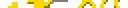
\includegraphics[width=.7\textwidth]{capitulos/capitulo4/new_1d.png}
			\caption{Distribución 1D de los \textit{tiles} en la OAM.}\label{fig:1d}
		\end{figure}

		\begin{figure}[h]
			\centering
			
\includegraphics[width=.4\textwidth]{capitulos/capitulo4/new_2d.png}
			\caption{Distribución 2D de los \textit{tiles} en la OAM.}\label{fig:2d}
		\end{figure}

	\item Bit \{5\}: Al activar este bit, el programador tendrá acceso a la OAM durante HBlank.
	\item Bit \{4\}: Permite la selección del buffer que se muestra por pantalla para los modos 4 y 5, los cuales manejan más de un buffer. Para más información consultar el punto~\ref{sec:mode_4} y~\ref{sec:mode_5}. 
	\item Bit \{3\}: La función que desempeña el tercer bit del registro DISPCNT es mostrar si el juego se está ejecutando en una Game Boy Color. El bit no se puede modificar. 
	\item Bits \{2-0\}: Modo del fondo utilizado. Entre los valores permitidos están el 0, 1 y 2, definidos para las tres maneras que tiene la GBA de procesar fondos. Los modos 3, 4 y 5 están reservados para los fondos bitmap. Los valores 6 y 7 no están permitidos. Las diferencias entre los modos se verán en las secciones~\ref{sec:bitmaps} y~\ref{sec:fondos}.
\end{itemize}

En la Tabla~\ref{tab:dispcnt} se hace un resumen de los parámetros del registro DISPCNT.

\begin{table}[h]
	\centering
	\begin{tabular}{| l | l |}
		\hline
		\textbf{Bits} & \textbf{Función}  \\ \hline
		F & Modo ``ventana'' para \textit{sprites}.  \\ \hline
		E-D & Modo ``ventana'' para fondos.  \\ \hline
		C & Activa el uso de \textit{sprites}.  \\ \hline
		B-8 & Activa cada uno de los 4 fondos disponibles.  \\ \hline
		7 & ``Reset'' de la pantalla.  \\ \hline
		6 & Especifica la distribución de los tiles en memoria. \\ \hline
		5 & Activa el acceso a la OAM durante HBlank. \\ \hline
		4 & Selecciona el buffer adicional en los modos 4 y 5. \\ \hline
		3 & Permite consultar si un juego se está ejecutando en una Game Boy Color. \\ \hline
		2-0 & Selecciona el modo que utiliza la Game Boy Advance para los fondos. \\ \hline
	\end{tabular}
	\caption{Registro \textit{Display Control}.}\label{tab:dispcnt}
\end{table}
\FloatBarrier{}

\subsubsection{DISPSTAT}

El siguiente registro, el \textit{Display Status} (conocido también como el registro DISPSTAT), se sitúa en la dirección de memoria 0x04000004 y permite al programador consultar la información relacionada con el VBlank, HBlank y VCount. VBlank es el período que hay entre cada fotograma refrescado, y HBlank se refiere al período que hay entre cada línea refrescada por pantalla. Por otro lado, VCount es el número de líneas, las filas de píxeles horizontales, refrescadas. Los bits que contiene son los siguientes:
\begin{itemize}
	\item Bits \{F-8\}: El programador especifica un valor VCount determinado, para invocar una interrupción en el bit {5} o que el cambio se vea reflejado en el bit {2}.
	\item Bit \{5\}: Activa la interrupción de VCount si este coincide con el valor especificado en {F-8}.
	\item Bits \{4-3\}: Activa la interrupción de HBlank y VBlank respectivamente.
	\item Bit \{2\}: Este bit tendrá valor si VCount coincide con el valor especificado en {F-8}.
	\item Bits \{1-0\}: Permiten saber si el dispositivo se encuentra en HBlank, si el valor del bit 0 es 1, o en VBlank, si el valor del bit 1 es 1.
\end{itemize}

En la Tabla~\ref{tab:dispstat} se hace un resumen de los parámetros del registro DISPSTAT.

\begin{table}[h]
	\centering
	\begin{tabular}{| l | l |}
		\hline
		\textbf{Bits} & \textbf{Función}  \\ \hline
		F-8 & VCount objetivo.  \\ \hline
		5 & Activa una interrupción al alcanzar VCount objetivo. \\ \hline
		4-3 & Activa la interrupción de HBlank y VBlank. \\ \hline
		2 & Bit activo en caso de alcanzar VCount objetivo.  \\ \hline
		1-0 & Esto de HBlank y VBlank. \\ \hline
	\end{tabular}
	\caption{Registro \textit{Display Status}.}\label{tab:dispstat}
\end{table}
\FloatBarrier{}

El valor de VCount también se puede consultar en la dirección de memoria 0x04000006. Dado que el valor oscila entre 0 y 227, solo se tienen en cuenta los primeros 8 bits.

\subsubsection{Configuración de fondos}\label{sec:conf_fondos}

A continuación, se detallan los registros para controlar los distintos parámetros que pueden tener los fondos de la Game Boy Advance. Estos registros sirven, entre otras cosas, para cambiar el tamaño, color y posicionamiento de los fondos.

\begin{itemize}
	\item Bits \{F-E\}: Tamaño del fondo. Para más información consultar la sección~\ref{sec:fondos}.
	\item Bit {D}: Por defecto, los fondos que no utilizan la matriz de transformación, se repiten en caso de que el \textit{offset} provoque que el fondo llegue a su fin. Este campo permite que los fondos que utilicen la matriz de transformación también se vean repetidos. Para más información, consultar el punto~\ref{sec:fondos}.
	\item Bits \{C-8\}: El índice del grupo de \textit{tiles} especifico que se utiliza.
	\item Bit {7}: Especifica el formato del color a utilizar. Con un 0 se consiguen 16 colores disponibles (4 bpp) y con un 1 se consiguen 256 colores (8 bpp).
	\item Bit {6}: Activa el modo mosaico. Más información en el punto~\ref{sec:sprites}.
	\item Bits \{3-2\}: Especifica el índice del bloque de grupo de \textit{tiles} a utilizar.
	\item Bits \{1-0\}: Prioridad de renderizado del fondo. Cuánto mayor sea el valor antes se renderizará en pantalla. En caso de que haya fondos con la misma prioridad se recurre al orden natural, siendo el primer fondo (BG0) el que mayor prioridad tiene y el último fondo el que menor prioridad tiene (BG3).
\end{itemize}

En la Tabla~\ref{tab:regfondo} se hace un resumen de los parámetros del registro de control de fondos.

\begin{table}[h]
	\centering
	\begin{tabular}{| l | l |}
		\hline
		\textbf{Bits} & \textbf{Función}  \\ \hline
		D & Activar la función ``wrap'' en las matrices que utilicen la matriz de transformación. \\ \hline
		C-8 & El índice del grupo de \textit{tiles} especifico que se utilizará.   \\ \hline
		7 & Rango de colores utilizado.  \\ \hline
		6 & Modo mosaico.  \\ \hline
		3-2 & Especifica el índice del bloque de grupo de \textit{tiles} que se utilizará. \\ \hline
		1-0 & Prioridad de renderizado. \\ \hline
	\end{tabular}
	\caption{Registro de control de fondos.}\label{tab:regfondo}
\end{table}
\FloatBarrier{}

Cada uno de los fondos cuenta con un registro de control específico. La ubicación de los registros para cada fondo se puede observar en la Tabla~\ref{tab:fondo_reg_1}. Además, en la tabla se incluye el \textit{offset} X e Y mencionado anteriormente.

En caso de que el programador quiera renderizar los fondos a través de una matriz de transformación dada (más información en el punto~\ref{sec:ppu}), tiene que configurar los registros de transformación y los registros de referencia. Este último sustituye a los parámetros de \textit{offset} vistos anteriormente para los fondos ``normales'' (aquellos que no utilicen la matriz de transformación).

\begin{table}[h]
	\centering
	\begin{tabular}{| l | l | l | l | l |}
		\hline
		\textbf{Fondos} & \textbf{Registro de Control} & \textbf{Registro de Offset X} & \textbf{Registro de Offset Y}  \\ \hline
		0 & 0x04000008 & 0x04000010 & 0x04000012  \\ \hline
		1 & 0x0400000A & 0x04000014 & 0x04000016  \\ \hline
		2 & 0x0400000C & 0x04000018 & 0x0400001A  \\ \hline
		3 & 0x0400000E & 0x0400001C & 0x0400001E  \\ \hline
	\end{tabular}
	\caption{Registros de cada uno de los fondos (1).}\label{tab:fondo_reg_1}
\end{table}
\FloatBarrier{}

El registro de transformación, como su nombre indica, se limita a almacenar los valores de la matriz de transformación. Los valores de la matriz 2x2 se almacenan consecutivamente, ocupando 2 bytes cada uno, empezando por 0x04000020 para el fondo 2 y 0x04000030 para el fondo 3 (véase la Tabla~\ref{tab:fondo_reg_2}). Estos valores son números \textit{fixed point} desplazados por 8 bits.

\begin{table}[h]
	\centering
	\begin{tabular}{| l | l | l | l | l |}
		\hline
		\textbf{Fondos} & \textbf{Registro de Transformación} & \textbf{Registro de Referencia}  \\ \hline
		0 &  - & -  \\ \hline
		1 & - & -  \\ \hline
		2 & 0x04000028-0x0400002E & 0x04000020-0x04000026  \\ \hline
		3 & 0x04000038-0x0400003E & 0x04000030-0x04000036  \\ \hline
	\end{tabular}
	\caption{Registros de cada uno de los fondos (2).}\label{tab:fondo_reg_2}
\end{table}

El otro registro a tener en cuenta, es el registro de referencia. Este replica el comportamiento del registro de \textit{offset} pero con números \textit{fixed point} de 28 bits. La distribución de los valores es la mostrada en la Tabla~\ref{tab:dist_fixed_fondo}.

\begin{table}[h]
	\centering
	\begin{tabular}{| l | l | l |}
		\hline
		27 & 26--8 & 7--0  \\ \hline
		Signo & Valor entero & Valor decimal  \\ \hline
	\end{tabular}
	\caption{Formato del valor de referencia de los fondos utilizando la matriz de transformación.}\label{tab:dist_fixed_fondo}
\end{table}

Los puntos de referencia X e Y para el fondo 2 se almacenan en las direcciones de memoria 0x04000028 y 0x0400002E respectivamente, mientras que los puntos de referencia X e Y para el fondo 3 se localizan en las direcciones de memoria 0x04000038 y 0x0400003E respectivamente (véase la Tabla~\ref{tab:fondo_reg_2}).

Como se puede apreciar en la Tabla~\ref{tab:fondo_reg_2}, los fondos 0 y 1 no cuentan con la posibilidad de poder utilizar la matriz de transformación.

\subsubsection{Registros de efectos especiales}

Finalmente, en la sección de registros LCD, las tres secciones que quedan son las del modo ventana, modo mosaico y otros efectos especiales. Las demostraciones de estas tres funciones se pueden ver en la Sección~\ref{sec:efectos}.

Dado que se pueden crear dos ventanas diferentes, existen dos registros distintos para cada uno, donde se especifican las dimensiones horizontales y verticales del rectángulo creado. Las dimensiones horizontales se indican en las direcciones 0x04000040 y 0x04000042 para las ventanas 0 y 1 respectivamente. De los 2 bytes que conforman cada valor, se utiliza 1 byte para cada una de las dos coordenadas X que representan las esquinas inferior izquierda y superior derecha del rectángulo. El formato para las coordenadas verticales es exactamente el mismo pero en las direcciones 0x04000044 para la ventana 0 y 0x04000046 para la ventana 1. En caso de que los valores superen la resolución del dispositivo (240x160), el valor introducido se interpreta como el máximo permitido. En el caso de la anchura, 240, y en el caso de la altura, 160. 

Sin embargo, antes de poder configurar las posiciones de las ventanas es necesario especificar cómo funcionan. Para ello se tiene que definir el comportamiento dentro de la ventanas, en el registro WININ en la dirección de memoria 0x04000048, y el comportamiento fuera de estas, en el registro WINOUT en la dirección de memoria 0x0400004A. Los parámetros para WININ son:

\begin{itemize}
	\item Bit \{D\}: Activa efectos especiales como el \textit{blending} y los efectos \textit{fade in} y \textit{fade out} para la ventana 1.
	\item Bit \{C\}: Activa el renderizado de \textit{sprites} para la ventana 1.
	\item Bits \{B-8\}: Activa los fondos 3, 2, 1 y 0, respectivamente, para la ventana 1.
	\item Bit \{5\}: Activa efectos especiales como el \textit{blending} y los efectos \textit{fade in} y \textit{fade out} para la ventana 0.
	\item Bit \{4\}: Activa el renderizado de \textit{sprites} para la ventana 0.
	\item Bits \{3-0\}: Activa los fondos 3, 2, 1 y 0, respectivamente, para la ventana 0.
\end{itemize}

Por otro lado, para controlar lo que se renderizá fuera de la ventana se configuran los siguientes parámetros en WINOUT:

\begin{itemize}
	\item Bit \{D\}: Activa efectos especiales fuera de las ventanas de \textit{sprites}.
	\item Bit \{C\}: Activa el renderizado de \textit{sprites} fuera de una ventana de \textit{sprites}.
	\item Bits \{B-8\}: Activa el renderizado de los fondos 3, 2, 1 y 0, respectivamente, fuera de una ventana de \textit{sprites}.
	\item Bit \{5\}: Activa efectos especiales fuera de las ventana de las de fondo.
	\item Bit \{4\}: Activa el renderizado de \textit{sprites} fuera de una ventana de fondo.
	\item Bits \{3-0\}: Activa el renderizado de los fondos 3, 2, 1 y 0, respectivamente, fuera de las ventanas de fondo.
\end{itemize}

El registro para la función mosaico se encuentra en la dirección de memoria 0x0400004C. El efecto distorsiona (o ``pixela'') la imagen dependiendo del valor que especifique el programador. Para una demostración del efecto consultar la Sección~\ref{sec:efectos}. Los bits que contiene son los siguientes:

\begin{itemize}
	\item Bits \{F-C\}: Distorsión en el eje vertical del \textit{sprite}.
	\item Bits \{B-8\}: Distorsión en el eje horizontal del \textit{sprite}.
	\item Bits \{7-4\}: Distorsión en el eje vertical del fondo.
	\item Bits \{3-0\}: Distorsión en el eje horizontal del fondo.
\end{itemize}

La última región de los registros LCD son aquellos dedicados al renderizado de efectos especiales. En concreto, los que permiten la mezcla de colores (o transparencia) y cambio de intensidad en la representación de los colores\footnote{Un incremento en la intensidad se traduce en una imagen más ``blanca'' mientras que una imagen con menos intensidad se traduce en una imagen más oscura.}.

El principal registro que gestiona toda la configuración relacionada con los efectos especiales es el registro posicionado en 0x04000050, denominado en~\cite{bib:gbatek} como BLDCNT. Los bits que contiene son los siguientes: 

\begin{itemize}
	\item Bits \{D-8\}: Selección de las capas posteriores a mezclar. Cada bit activa el ``backdrop''\footnote{El ``backdrop'' de la GBA consiste en un fondo completamente negro.}, \textit{sprites} y fondos 3, 2, 1 y 0, respectivamente.
	\item Bits \{7-6\}: Selección del efecto a procesar. Siendo 3, se traduce en un incremento en la intensidad de la capa frontal. Si es 2, se hace una disminución en la intensidad de la capa frontal Cuando es 1, se hace una mezcla de colores de las capas frontales con las posteriores seleccionadas. Finalmente, el 0 significa que no se escoge ningún efecto. Para que la mezcla de colores funcione como se espera es necesario que la capa frontal se encuentre, como su nombre indica, por encima de la capa (o capas) posteriores. 
	\item Bits \{5-0\}: Selección de las capas frontales a mezclar. Cada bit activa el ``backdrop'', \textit{sprites} y fondos 3, 2, 1 y 0, respectivamente.
\end{itemize}

Para poder procesar los efectos tal y como desea el programador, este tiene que especificar los valores adecuados en los registros BLDALPHA para configurar el nivel de mezcla entre las capas frontales y posteriores, en 0x0400052. De forma adicional, para controlar el nivel de intensidad en las capas seleccionadas, tendrá que modificar el valor de BLDY en 0x04000054.

En el caso del registro BLDALPHA, que ocupa 2 bytes, los bits \{C-8\} denotan el coeficiente que tendrán las capas posteriores mientras que los bits \{4-0\} indican el coeficiente que tendrán las capas frontales. De forma similar a lo que ocurre con los registros de los fondos que utilizan las matrices de transformación, los 4 bits inferiores de cada coeficiente simbolizan incrementos fraccionales de $1/16$, teniendo cada coeficiente un rango entre 0 y 1. En el caso del registro BLDY, ocurre lo mismo pero solo utilizando los bits \{4-0\} para especificar un valor entre 0 y 1.

\subsection{Registros de sonido}

La Game Boy Advance ofrece 6 modos diferentes de sonido, 4 analógicos y 2 digitales (canales A-B). Hay un registro para controlar cada uno de ellos además de varios generales que controlan el volumen.

El término técnico para referirse a las 6 opciones de la consola para ofrecer audio es ``canal''. Sin embargo, para no confundirlo con los canales de izquierda y derecha, a lo largo del trabajo, se hará referencia a los 6 canales como ``modos''.

La información contenida en esta sección se basa en la documentación oficial~\cite{bib:gba_manual} y en el material adicional disponible en~\cite{bib:belogic}.

\subsubsection{Modos analógicos}
Los dos primeros modos que ofrece el hardware de la consola, los canales 1 y 2, permiten la reproducción de pulsos con la posibilidad de modificar el volumen de cada onda. De forma adicional, el primer modo permite cambiar de dinámicamente la frecuencia de las ondas. Para ello, ambos modos harán uso de registros para modificar el tono y la duración de la onda, teniendo el modo 1 un registro adicional para controlar la frecuencia. 

El registro encargado de la duración, volumen y ciclo de la onda utiliza el siguiente formato para los modos 1 y 2:

\begin{itemize}
	\item Bits \{F-C\}: Volumen inicial del sonido.
	\item Bit \{B\}: Modificación del volumen. 0 para disminuirlo conforme pasa el tiempo y 1 para incrementarlo conforme pasa el tiempo. 
	\item Bits \{A-8\}: El período con el que cambia el volumen. El valor especificado resulta en $n/64$ segundos de período. 
	\item Bits \{7-6\}: El ciclo que toma el pulso. 0 para un ciclo del 12.5\%, 1 para un ciclo del 25\%, 2 para un ciclo del 50\% y 3 para un ciclo del 75\%.
	\item Bits \{5-0\}: La duración del sonido. El valor especificado resulta en $(64-n)/256$ segundos.
\end{itemize}

El registro encargado de la frecuencia de la onda utiliza el siguiente formato para los modos 1 y 2:

\begin{itemize}
	\item Bit \{F\}: En caso de estar activo el bit, ``resetea'' el sonido.
	\item Bit \{E\}: En caso de ser 0, el sonido es reproducido de forma constante. Si es 1, el sonido es reproducido con la duración especificada en los bits \{5-0\} del registro anterior.
	\item Bits \{A-0\}: Frecuencia utilizada para el tono. El valor especificado resulta en $131072/(2048-n)$ Hz.
\end{itemize}

Para indicar un cambio dinámico en la frecuencia, el modo 1 cuenta con el registro ``sweep'', que tiene los siguientes bits:

\begin{itemize}
	\item Bits \{6-4\}: El tiempo que pasa entre cambios de frecuencia. El valor especificado resulta en $n/128$ segundos.
	\item Bit \{3\}: Cómo se modifica la frecuencia. 0 para el incremento con el paso del tiempo y 1 para la disminución.
	\item Bits \{2-0\}: Denota el cambio en la frecuencia. El valor especificado resulta en un cambio en el periodo de $T=T\pm{}T/2^n$. La suma o resta dependerá del valor del bit {3}.
\end{itemize}

En la Tabla~\ref{tab:reg_canal_1_2} se incluyen los registros de los modos 1 y 2.

\begin{table}[h]
	\centering
	\begin{tabular}{| l | l | l | l |}
		\hline
		\textbf{Canal} & \textbf{Registro de duración} & \textbf{Registro de frecuencia} & \textbf{Registro ``sweep''} \\ \hline
		1 & 0x04000062 & 0x04000064 & 0x04000060 \\ \hline
		2 & 0x04000068 & 0x0400006C & - \\ \hline
	\end{tabular}
	\caption{Registros dedicados de los modos 1 y 2.}\label{tab:reg_canal_1_2}
\end{table}
\FloatBarrier{}

El modo 3, permite reproducir ondas almacenadas en el espacio de memoria localizado entre 0x04000090 y 0x0400009F. En este modo se pueden diferenciar los registros de control para la selección, duración y frecuencia.

El primer registro, reservado para seleccionar la muestra localizada en [0x04000090, 0x0400009F] y utilizado para activar el modo, tiene el siguiente formato:

\begin{itemize}
	\item Bit \{7\}: Activa el modo.
	\item Bit \{6\}: Selecciona el grupo a utilizar. Complementa al bit {5}.
	\item Bit \{5\}: En caso de que el valor sea 0, la Game Boy Advance dividirá las ondas almacenadas en el rango de memoria especificado anteriormente en dos grupos diferentes de 32 muestras cada una. En caso de ser 1, gestionará toda la información almacenada en el rango como un solo grupo de 64 muestras.
\end{itemize}

El segundo registro, es el encargado de modificar la duración y el volumen del modo 3:

\begin{itemize}
	\item Bits \{F-D\}: Volumen del modo. 0 para 0\%, 1 para 100\%, 4 para 75\%, 2 para 50\% y 3 para el 25\%.
	\item Bits \{7-0\}: La duración del sonido. El valor especificado resulta en $n/256$ segundos.
\end{itemize}

Finalmente, el tercer registro necesario para utilizar el modo 3 es el encargado de configurar la frecuencia y repetición del sonido. Tiene el mismo formato descrito para los modos 1 y 2, y cuenta con los siguientes bits:

\begin{itemize}
	\item Bit \{F\}: En caso de estar activo el bit, ``resetea'' el sonido.
	\item Bit \{E\}: Si es 0, reproduce el sonido de forma constante. Si es 1, reproduce el sonido con la duración especificada en los bits \{5-0\} del registro anterior.
	\item Bits \{A-0\}: Frecuencia utilizada para el tono. El valor especificado resulta en $131072/(2048-n)$ Hz.
\end{itemize}

El último modo analógico, el modo 4, tiene como función generar ruido como añadido a los demás modos. De los dos registros reservados para el modo, el que controla la duración y el volumen sigue el mismo formato presentado anteriormente. El registro diferente que se introduce en este caso, es el registro de ruido, que tiene la siguiente estructura:

\begin{itemize}
	\item Bit \{F\}: En caso de estar activo el bit, ``resetea'' el sonido.
	\item Bit \{E\}: Si es 0, reproduce el sonido de forma constante. Si es 1, reproduce el sonido con la duración especificada en los bits \{5-0\} del registro anterior.
	\item Bits \{7-4\}: Denota la función a utilizar con la frecuencia especificada en los bits \{2-0\}. La salida de la función (o \textit{pre-scaler divider} como se llama en~\cite{bib:belogic}) será utilizada para generar el ruido. El efecto del valor del campo sobre la función se puede observar en la ecuación~\ref{eq:fn_canal_4}.

	\begin{align}
		Q/2^{valor+1}
		\label{eq:fn_canal_4}
	\end{align}

	\item Bit \{3\}: Controla el período del ruido generado. Si es 0, el periodo es de 127 ciclos y si es de 1, el periodo es de 32767 ciclos.
	\item Bits \{2-0\}: Frecuencia utilizada en conjunto con la función denotada en [7-4] para generar ruido. Las frecuencias vinculadas a los 8 valores disponibles se pueden observar en la Tabla~\ref{tab:frec_canal_4}.

	\begin{table}[h]
		\centering
		\begin{tabular}{| l | l |}
			\hline
			\textbf{Valor} & \textbf{Frecuencia (en MHz)}  \\ \hline
			0 & $4.19304/2$ \\ \hline
			1 & $4.19304/8$ \\ \hline
			2 & $4.19304/16$ \\ \hline
			3 & $4.19304/24$ \\ \hline
			4 & $4.19304/32$ \\ \hline
			5 & $4.19304/40$ \\ \hline
			6 & $4.19304/48$ \\ \hline
			7 & $4.19304/56$ \\ \hline
		\end{tabular}
		\caption{Frecuencias disponibles para generar ruido en el modo 4.}\label{tab:frec_canal_4}
	\end{table}
	\FloatBarrier{}
\end{itemize}

\subsubsection{Modos digitales}
Se introdujeron dos nuevos modos con respecto al sistema de audio de la Game Boy Color. Estos modos, denominados A y B, hacen uso de los dos DACs (Conversor Digital Analógico) de 8 bits incorporados en la consola. Para utilizarlos se distinguen dos tipos de registros, aquellos reservados para indicar los datos a usar y otros para configurar los modos, los registros de control.

Los registros de datos de los modos A y B, se encuentran en las regiones 0x040000A0 y 0x040000A4, respectivamente. El sistema que implementa la Game Boy Advance, denominado Direct Sound, coge los primeros datos que encuentra en el buffer (FIFO), es decir, los 8 bits menos significativos del registro de 32 bits, que serán los primeros en reproducirse. Para activar la salida de sonido de estos modos, y también los modos 1-4, se utilizan tres registros de control. El primero está en 0x04000080 y tiene como función activar y controlar de forma global el volumen de los modos 1-4. Tiene el siguiente formato:

\begin{itemize}
	\item Bits \{F-C\}: Cada uno de los 4 bits activa el canal izquierdo para los modos 1-4.
	\item Bits \{B-8\}: Cada uno de los 4 bits activa el canal derecho para los modos 1-4.
	\item Bits \{6-4\}: Volumen en el canal izquierdo de los primeros 4 modos.
	\item Bits \{2-0\}: Volumen en el canal derecho de los primeros 4 modos.  
\end{itemize}

El segundo registro de control utilizado es el posicionado en la dirección de memoria 0x04000082. Este modifica el volumen global de los modos 1-4 para los dos canales, además de configurar parámetros relacionados con los modos A y B. Tiene el siguiente formato:

\begin{itemize}
	\item Bit \{F\}: Restablece el buffer de datos FIFO del modo B.
	\item Bit \{E\}: Para poder reproducir sonido en los modos A y B, es necesario utilizar el temporizador 0 o 1. En este campo se especifica cual de los dos temporizadores se utilizará para el modo B.
	\item Bits \{D-C\}: Activa los canales izquierdo (2) y/o derecho (1) del modo B.
	\item Bit \{B\}: Restablece el buffer de datos FIFO del modo A.
	\item Bit \{A\}: Al igual que en el campo {E} se especifica el temporizador a utilizar para el modo A, número 0 o 1.
	\item Bits \{9-8\}: Activa los canales izquierdo (2) y/o derecho (1) del modo A.  
	\item Bit \{3\}: Volumen global del modo B.  
	\item Bit \{2\}: Volumen global del modo A.  
	\item Bits \{1-0\}: Volumen global de los primeros 4 modos. 
\end{itemize}

Finalmente, el registro denominado el ``master switch'' se posiciona en la dirección de memoria 0x04000084. El registro también puede servir para consultar el estado actual en el que se encuentran los modos 1-4. Es importante mencionar que los bits destinados a consultar el estado actual de un modo no pueden ser sobrescritos por el programador.

\begin{itemize}
	\item Bit \{7\}: Permite desactivar todos los modos que ofrece la Game Boy Advance al igualar el campo a 0.
	\item Bits \{3-0\}: Especifica el estado de los modos 4, 3, 2 y 1, respectivamente. Un valor igual a 1 denota que el estado está activo, mientras que el 0 indica lo contrario.
\end{itemize}

\subsection{Registros para \textit{Direct Memory Access}}
La GBA ofrece la posibilidad de copiar datos rápidamente de una dirección de memoria a otra mediante el uso de \textit{Direct Memory Access} (DMA)~\cite{bib:dma_book}.

La consola cuenta con 4 variantes de \textit{DMA} con diferentes prioridades y, por ende, finalidades. El canal número 0 permite realizar transferencias con la máxima prioridad disponible. Los canales 1 y 2 se reservan para las transferencias de sonido a los buffers adecuados. Por último, el canal 3 se reserva para transferencias generales.

Los registros de 32 bits que permiten llevar a cabo estas operaciones son los registros fuente, destino y de control \textit{DMA}. Estos tres registros se repiten para cada uno de los 4 canales. En concreto, el registro de control \textit{DMA} sigue el formato descrito a continuación:

\begin{itemize}
	\item Bit \{1F\}: Activa una transferencia mediante \textit{DMA}.
	\item Bit \{1E\}: Activa una interrupción en caso de haberse completado la operación. 
	\item Bits \{1D-1C\}: Especifica cuándo debe comenzar la transferencia: 0 de manera inmediata, 1 al entrar en el estado VBlank, 2 al entrar en el estado HBlank y el comportamiento al igualar a 3 dependerá del canal utilizado. Para los canales reservados para audio se empieza la transferencia una vez que se hayan leído los buffers correspondientes. Para el canal 3 se realiza una transferencia antes de que la \textit{PPU} renderice cada línea horizontal de la pantalla~\cite{bib:tonc}.
	\item Bit \{1A\}: Especifica el tamaño del dato a copiar. 0 para 16 bits y 1 para 32 bits. 
	\item Bit \{19\}: Si se ha seleccionado el modo 1 en los bits \{1D-1C\}, se repite la transferencia cada vez que el dispositivo entre en el estado VBlank. En el caso de haber seleccionado el modo 2 en los bits \{1D-1C\}, se repite la transferencia cada vez que el dispositivo entre en el estado HBlank.
	\item Bits \{18-17\}: Definen la modificación de la dirección fuente que se lleva a cabo al completar una copia: 0 para incrementar la dirección fuente, 1 para decrementar la dirección fuente, 2 para dejar la dirección de destino fija y 3 para incrementar la dirección fuente, restableciendo el valor inicial una vez acabada la operación. 
	\item Bits \{16-15\}: La finalidad de estos dos bits es similar a la mostrada en los bits \{18-17\} pero para la dirección destino.
	\item Bits \{0F-00\}: El número de transferencias realizadas en la operación.
\end{itemize}

Los registros de fuente y destino restantes se configuran simplemente igualando el valor del registro a la dirección de memoria correspondiente. La dirección de memoria para canal quedaría tal y como se muestra en la Tabla~\ref{tab:dma}.

\begin{table}[h]
	\centering
	\begin{tabular}{| l | l | l | l |}
		\hline
		\textbf{Canal} & \textbf{Registro fuente} & \textbf{Registro destino} & \textbf{Registro de control}  \\ \hline
		0 &  0x040000B0 & 0x040000B4 & 0x040000B8 \\ \hline
		1 &  0x040000BC & 0x040000C0 & 0x040000C4 \\ \hline
		2 &  0x040000C8 & 0x040000CC & 0x040000D0 \\ \hline
		3 &  0x040000D4 & 0x040000D8 & 0x040000DC \\ \hline
	\end{tabular}
	\caption{Registros fuente, destino y de control de \textit{DMA}.}\label{tab:dma}
\end{table}
\FloatBarrier{}

Las transferencias que utilizan \textit{DMA}, a pesar de ser más rápidas que las funciones \textit{memcpy} y \textit{memset} convencionales, traen consigo problemas adicionales que pueden causar un comportamiento inesperado. Por ejemplo, al poner a la CPU en un estado ``inerte'', cualquier tipo de interrupción configurada se puede ver afectada~\cite{bib:tonc}.

Finalmente, es importante comentar que el canal 0 únicamente puede copiar desde la RAM interna del dispositivo.

\subsection{Registros de temporización}
La Game Boy Advance ofrece la posibilidad de configurar hasta 4 contadores independientes que permitan un seguimiento del tiempo. Los dos tipos de registros que se diferencian en esta sección, son los registros de control y de datos. Cada uno ocupa 2 bytes~\cite{bib:tonc}. 

El registro de control tiene el siguiente formato:

\begin{itemize}
	\item Bit \{7\}: Activa el temporizador.
	\item Bit \{6\}: Activa la interrupción cuando el temporizador sobrepasa el límite. 
	\item Bit \{2\}: Hace que los ``overflows'' de temporizadores posicionados previamente en memoria incrementen el valor del temporizador. Por ejemplo, si el valor objetivo se alcanza en el temporizador 2, el temporizador 3 incrementará su valor. 
	\item Bits \{1-0\}: Define la frecuencia con la que se actualiza el contador: 0 para una frecuencia de 16.78 MHz, 1 para 262.21 KHz, 2 para 65.536 KHz y 3 para 16.384 KHz. El programador puede conseguir de manera exacta la frecuencia con la que se actualizan los valores especificando un ``offset'' en el registro de datos~\cite{bib:tonc}.
\end{itemize}

El registro de datos complementa al registro de control y permite tanto la lectura del valor actual del contador como la escritura del valor inicial del contador. El valor que provocará el ``overflow'' viene dado por la ecuación~\ref{eq:eq_temporizador}. Dado que el programador puede especificar un valor inicial, no siempre se producirá un ``overflow'' a los 65536 incrementos.

\begin{align}
	65536 - n_{inc} = 0
	\label{eq:eq_temporizador}
\end{align}

El formato de ambos registros se utiliza repetidamente para cubrir cada uno de los 4 temporizadores. Las direcciones de memoria de los registros de control y de datos para cada temporizador se pueden observar en la Tabla~\ref{tab:temporizadores}.

\begin{table}[h]
	\centering
	\begin{tabular}{| l | l | l |}
		\hline
		\textbf{Temporizador} & \textbf{Registro de Control} & \textbf{Registro de Datos}  \\ \hline
		0 &  0x04000102 & 0x04000100  \\ \hline
		1 &  0x04000106 & 0x04000104  \\ \hline
		2 &  0x0400010A & 0x04000108  \\ \hline
		3 &  0x0400010E & 0x0400010C  \\ \hline
	\end{tabular}
	\caption{Registros de control y datos de los temporizadores.}\label{tab:temporizadores}
\end{table}
\FloatBarrier{}

\subsection{Registros de comunicación serie}
La Game Boy Advance permite el intercambio de información con otras GBAs a partir del puerto serie que trae cada una de sus tres variantes. En concreto, la consola ofrece 6 modos diferentes en los que otro dispositivo puede interactuar con la consola. Sin embargo, en este apartado solo se comentarán brevemente el modo normal, que permite la comunicación bidireccional entre dos consolas y unidireccional entre varias GBA; y el modo multijugador, el cual permite la comunicación bidireccional entre un máximo de 4 consolas Game Boy Advance.

Tanto el modo normal como el multijugador precisa del registro de control general de comunicación (llamado RCNT según \cite{bib:gbatek}) y el registro de control de entrada y salida serie (SIOCNT).

En los dos modos es necesario inicializar el registro RCNT (posicionado en la dirección de memoria 0x04000134) a los valores mostrados a continuación:

\begin{itemize}
	\item Bit \{F\}: Su valor debe ser 0 para poder utilizar cualquiera de los dos modos de comunicación.
	\item Bit \{E\}: A pesar de no tener un uso (por lo menos documentado) su valor debe ser 0.
	\item Bits \{8-4\}: A pesar de no tener un uso (por lo menos documentado) su valor debe ser 0.
	\item Bits \{3-0\}: Es irrevelante para los modos descritos en esta sección.
\end{itemize}

El registro SIOCNT, en el que sí hay diferencias entre los dos modos, se ubica en la dirección de memoria 0x04000128. Para el modo normal, el registro sigue el siguiente formato:

\begin{itemize}
	\item Bit \{E\}: Activa la interrupción de comunicación serie en caso de haberse completado una transferencia.
	\item Bit \{D\}: Se hace 0 para activar la comunicación en modo normal y 1 para activar la comunicación en modo multijugador.
	\item Bit \{C\}: El campo configura el tamaño de la transferencia, 0 para 8 bits y 1 para 32 bits.
	\item Bit \{7\}: Especifica el estado actual de la comunicación, 0 denota un estado inactivo y 1 un estado activo.
	\item Bit \{3\}: Estado de salida de datos.
	\item Bit \{2\}: Estado de entrada de datos. Se traduce en el estado del bit \{3\} de los demás dispositivos.
	\item Bit \{1\}: Define la frecuencia a la que funciona la comunicación. Es 0 para 256 KHz y 1 para 2 MHz. Para conseguir estabilidad en la transferencia de datos se recomienda una frecuencia de 256 KHz dado que la transferencia a 2 MHz se reserva para hardware especial \cite{bib:gbatek}.
	\item Bit \{0\}: Indica el reloj utilizado como referencia para la transferencia. Es 0 para el reloj externo y 1 para el interno.
\end{itemize}

El modo multijugador sigue un formato parecido excepto por los valores posicionados en el primer byte del registro. Concretamente, se sigue el siguiente formato:

\begin{itemize}
	\item Bit \{E\}: Activa la interrupción de la comunicación serie en caso de haberse completado una transferencia.
	\item Bit \{D\}: Se hace 0 para activar la comunicación en modo normal y 1 para activar la comunicación en modo multijugador.
	\item Bit \{C\}: Para poder utilizar el modo multijugador el valor debe ser 0.
	\item Bit \{7\}: Especifica el estado actual de la comunicación. Se pone a 0 para indicar un estado inactivo y a 1 para un estado activo. En el caso del modo multijugador, este bit no se puede modificar en los dispositivos esclavos conectados a la GBA principal.
	\item Bit \{6\}: El valor es 1 en caso de haberse producido un error.
	\item Bits \{5-4\}: El valor define el rol que toma el dispositivo en la comunicación. Es 0 para el dispositivo principal, y 1, 2 y 3 para los dispositivos esclavos.
	\item Bit \{3\}: Estado de la conexión. El valor 0 denota un fallo en la conexión, mientras que el 1 indica que todos los demás dispositivos están listos. 
	\item Bit \{2\}: Es similar a los bits \{5-4\}. Denota si el dispositivo tiene el rol maestro (1) o de esclavo (0).
	\item Bits \{1-0\}: Indica la tasa de baudios a la que se envían los datos. Es 0 para 9600, 1 para 38400, 2 para 57600 y 3 para 115200 bps.
\end{itemize}

Los siguientes registros a tener en cuenta son los encargados de enviar los datos a los diferentes dispositivos.  

En el caso del modo normal se pueden distinguir dos registros, uno dedicado a las transferencias de 8 bits (en la dirección de memoria 0x0400012A) y otro para las transferencias de 32 bits (en la dirección de memoria 0x04000122). En el registro de 8 bits, únicamente se almacenarán los 8 bit menos significativos. Para garantizar el correcto funcionamiento de la comunicación, los dos registros deben contener la información a enviar antes de activar la comunicación serie. Al terminar, la información recibida acaba sustituyendo los datos iniciales escritos en ambos registros.

Por otro lado, el modo multijugador, cuenta con un registro específico para el envío de datos, que reutiliza el registro destinado a transferencias de 8 bits en el modo normal, pero esta vez utilizando completamente los 16 bits del registro. Además, se incluyen registros para recibir los datos de cada uno de los roles en una comunicación serie multijugador. La distribución de estos se puede ver en la Tabla~\ref{tab:mult_modo}.

\begin{table}[h]
	\centering
	\begin{tabular}{| l | l |}
		\hline
		\textbf{Dispositivo} & \textbf{Registro I/O para el modo multijugador} \\ \hline
		0 (Máster) &  0x04000120 \\ \hline
		1 (Esclavo) &  0x04000122 \\ \hline
		2 (Esclavo) &  0x04000124 \\ \hline
		3 (Esclavo) &  0x04000126 \\ \hline
	\end{tabular}
	\caption{Registros I/O para el modo multijugador.}\label{tab:mult_modo}
\end{table}
\FloatBarrier{}

\subsection{Registros de los botones}
El dispositivo ofrece dos formas de obtener la entrada del usuario:

\begin{itemize}
	\item La primera es comprobar directamente el registro KEYINPUT, posicionado en la dirección 0x04000130. Este registro ocupa 2 bytes, aunque solo son útiles los primeros 10 bits. La distribución de los botones de la consola se puede observar en la Tabla~\ref{tab:keypad_reg}. Al consultar los valores del registro es necesario tener en cuenta que un 0 en un bit determinado significa que el botón ha sido pulsado, mientras que un 1 indica lo contrario.
	\item La segunda forma, únicamente recomendada para hacer que el dispositivo salga de un estado de bajo consumo, se basa en el uso de interrupciones. Para ello, el programador tendrá que configurar el registro KEYCNT (véase la Tabla~\ref{tab:keypad_irq_reg}), ubicado en la dirección de memoria 0x04000132.
\end{itemize}

	\begin{table}[h]
		\centering
		\begin{tabular}{| l | l |}
			\hline
			\textbf{Bit} & \textbf{Botón} \\ \hline
			9 &  L \\ \hline
			8 &  R \\ \hline
			7 &  Abajo (D-pad) \\ \hline
			6 &  Arriba (D-pad) \\ \hline
			5 &  Izquierda (D-pad) \\ \hline
			4 &  Derecha (D-pad) \\ \hline
			3 &  Start \\ \hline
			2 &  Select \\ \hline
			1 &  B \\ \hline
			0 &  A \\ \hline
		\end{tabular}
		\caption{Los botones en el registro KEYINPUT.}\label{tab:keypad_reg}
	\end{table}

	\begin{longtable}[h]
		\centering
		\begin{tabular}{| l | p{5cm} |}
			\hline
			\textbf{Bit} & \textbf{Función} \\ \hline
			F &  La condición que se debe cumplir para que se active la interrupción. 0 para que se active con tener pulsado uno de los botones activados y 1 para que se active con tener pulsado todos los botones activados. \\ \hline
			E &  Activa la interrupción de botones de la Game Boy Advance. \\ \hline
			9 &  Se tiene en cuenta el botón L para la interrupción. \\ \hline
			8 &  Se tiene en cuenta el botón R para la interrupción. \\ \hline
			7 &  Se tiene en cuenta el botón de abajo (D-pad) para la interrupción. \\ \hline
			6 &  Se tiene en cuenta el botón de arriba (D-pad) para la interrupción. \\ \hline
			5 &  Se tiene en cuenta el botón de izquierda (D-pad) para la interrupción. \\ \hline
			4 &  Se tiene en cuenta el botón de derecha (D-pad) para la interrupción. \\ \hline
			3 &  Se tiene en cuenta el botón Start para la interrupción. \\ \hline
			2 &  Se tiene en cuenta el botón Select para la interrupción. \\ \hline
			1 &  Se tiene en cuenta el botón B para la interrupción. \\ \hline
			0 &  Se tiene en cuenta el botón A para la interrupción. \\ \hline
		\end{tabular}
		\caption{Los botones en el registro KEYCNT.}\label{tab:keypad_irq_reg}
	\end{longtable}
	\FloatBarrier{}

\subsection{Registros de interrupciones}
Para activar y utilizar las interrupciones en el dispositivo, el programador precisará de tres registros: IME, IE e IF.

El primero, el registro IME (\textit{Interrupt Master Enable Register}), es el encargado de activar el uso de interrupciones en el sistema. De los 4 bytes que ocupa el registro, solo se utiliza el primer bit, para denotar si se utilizan interrupciones o no.

En caso de activar el uso de interrupciones, el programador tendrá que especificar cuáles hay que utilizar. Para ello tendrá que modificar los valores del registro IE (\textit{Interrupt Enable Register}) para indicar cuáles de las 14 interrupciones disponibles serán utilizadas (véase la Tabla~\ref{tab:irq_ie}).

\begin{table}[h]
	\centering
	\begin{tabular}{| l | p{15cm} |}
		\hline
		\textbf{Bit} & \textbf{Interrupción} \\ \hline
		D &  Activa la interrupción al retirar el cartucho de la consola. \\ \hline
		C &  Activa la interrupción para la detección de los botones especificada en el registro KEYCNT. \\ \hline
		B &  Activa la interrupción al completar la transferencia número 3 a través de DMA. \\ \hline
		A &  Activa la interrupción al completar la transferencia número 2 a través de DMA. \\ \hline
		9 &  Activa la interrupción al completar la transferencia número 1 a través de DMA. \\ \hline
		8 &  Activa la interrupción al completar la transferencia número 0 a través de DMA. \\ \hline
		7 &  Activa la interrupción al completar una transferencia por comunicación serie. \\ \hline
		6 &  Activa la interrupción cuando se sobrepasa el temporizador número 3. \\ \hline
		5 &  Activa la interrupción cuando se sobrepasa el temporizador número 2. \\ \hline
		4 &  Activa la interrupción cuando se sobrepasa el temporizador número 1. \\ \hline
		3 &  Activa la interrupción cuando se sobrepasa el temporizador número 0. \\ \hline
		2 &  Activa la interrupción cuando el valor de VCount objetivo especificado en el registro DISPSTAT es alcanzado. \\ \hline
		1 &  Activa la interrupción cuando se entra en la región HBlank de la pantalla. \\ \hline
		0 &  Activa la interrupción cuando se entra en la región VBlank de la pantalla. \\ \hline
	\end{tabular}
	\caption{Interrupciones disponibles en el sistema.}\label{tab:irq_ie}
\end{table}

Sin embargo, una vez provocada la interrupción, el programador tendrá que hacerle saber a la máquina que la interrupción ha sido gestionada exitosamente. El registro donde se realiza esta acción es el IF (\textit{Interrupt Request Flags}), en la dirección de memoria 0x04000202. Siguiendo el mismo formato mostrado en la Tabla~\ref{tab:irq_ie}, se tendrá que escribir un 1 en el bit de la interrupción gestionada. Todo esto se hace desde la función que el programador tendrá que especificar en la dirección de memoria 0x03007FFC.

\section{\textit{Picture Processing Unit} (PPU)}\label{sec:ppu}

La unidad de procesamiento de imágenes de la Game Boy Advance procesa la información de las secciones OAM, VRAM y RAM de paleta, mostradas en la Tabla~\ref{tab:mapa}, para producir una imagen que el jugador pueda ver. En la Sección~\ref{sec:arquitectura} se detallaron los modos existentes según la PPU trata lo datos. Diferenciamos tres: \textbf{\textit{Sprites}}, \textbf{\textit{Bitmaps}} y \textbf{Fondos} \cite{bib:gba_manual}. En las próximas secciones se comentarán cada uno de estos modos y sus diferentes variaciones y configuraciones.

Sin embargo, antes de indagar en cada uno de los modos hace falta entender conceptos como los \textit{tiles}. Estos son necesarios al hablar de los modos de \textit{sprites} y \textit{fondos}, la forma en la que el programador posiciona los píxeles y objetos en pantalla, y el formato utilizado para representar colores en la consola. Todos son conceptos indispensables para cualquiera de los modos que ofrece la consola de Nintendo.

Los \textit{tiles} denotan unas pequeñas imágenes (normalmente cuadradas) que sirven como base para crear escenarios y personajes. Para facilitar la comprensión de este proceso, se muestra a continuación un ejemplo en \textit{Tiled} (véase sección~\ref{sec:herr_graficas}) donde se crea un escenario (o fondo) a partir de imágenes base de un tamaño de 32 x 32 píxeles. Al conjunto de imágenes base (\textit{tiles}) se le denomina \textit{tileset}. En la Figura~\ref{fig:tiled_demo_1} se muestra un \textit{tileset} en el que se puede distinguir cada unidad por la separación que hace \textit{Tiled}.

A partir de este conjunto de imágenes base, se crea la imagen final. El proceso se puede observar en las Figuras~\ref{fig:tiled_demo_2} y~\ref{fig:tiled_demo_3}.

\begin{figure}[h]
	\centering
	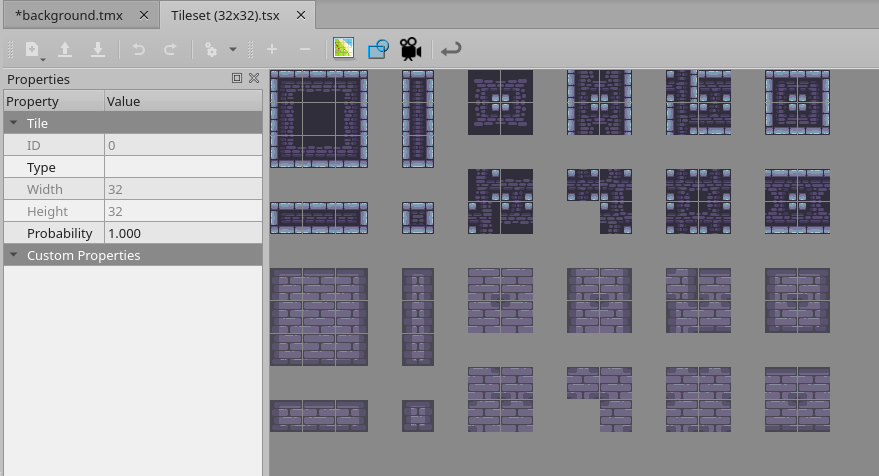
\includegraphics[width=.7\textwidth]{capitulos/capitulo3/tiled_demo_1.png}
	\caption{\textit{Tileset} que se utilizará para crear el fondo.}
	\label{fig:tiled_demo_1}
\end{figure}

\begin{figure}[h]
	\centering
	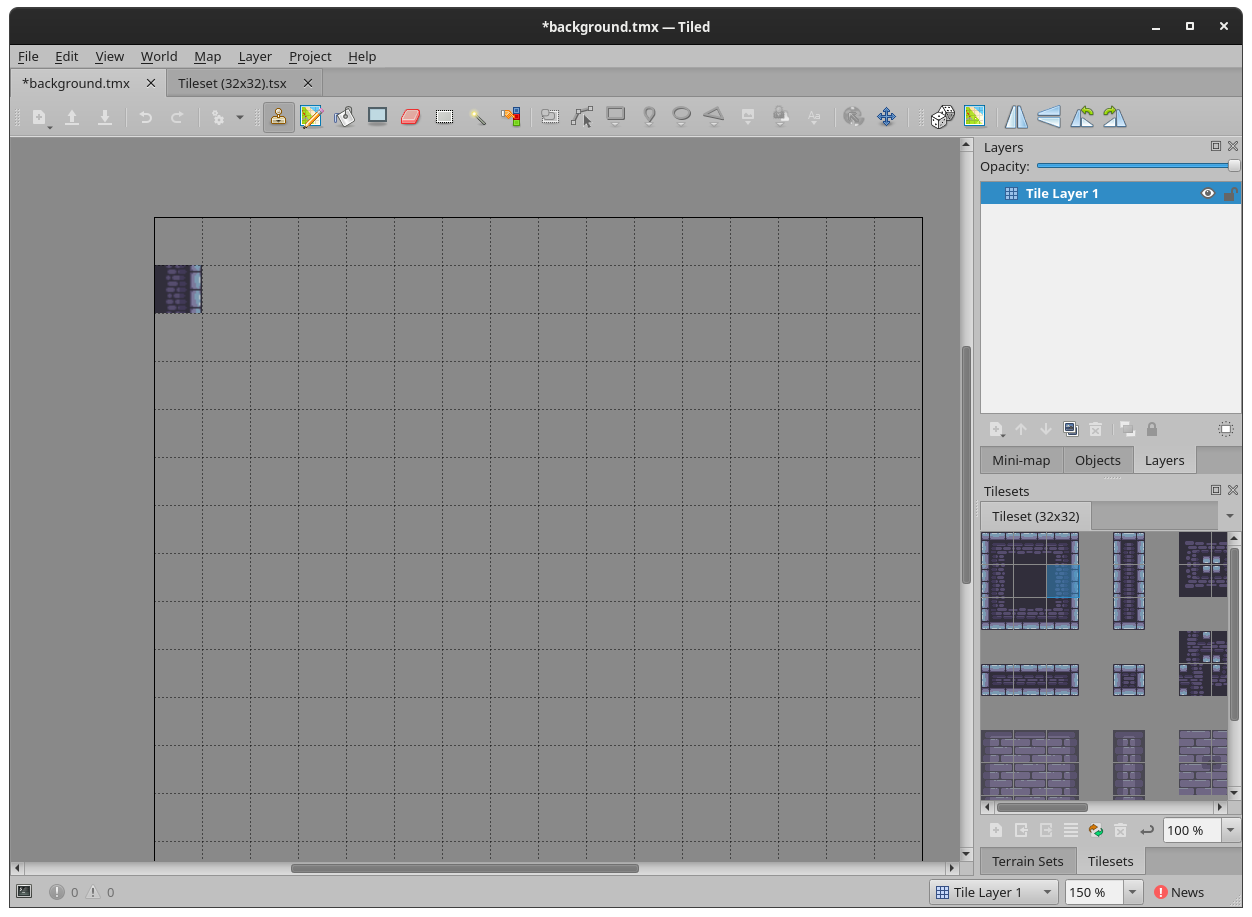
\includegraphics[width=.6\textwidth]{capitulos/capitulo3/tiled_demo_2.png}
	\caption{Relleno del canvas a partir de \textit{tiles}.}
	\label{fig:tiled_demo_2}
\end{figure}

\begin{figure}[h]
	\centering
	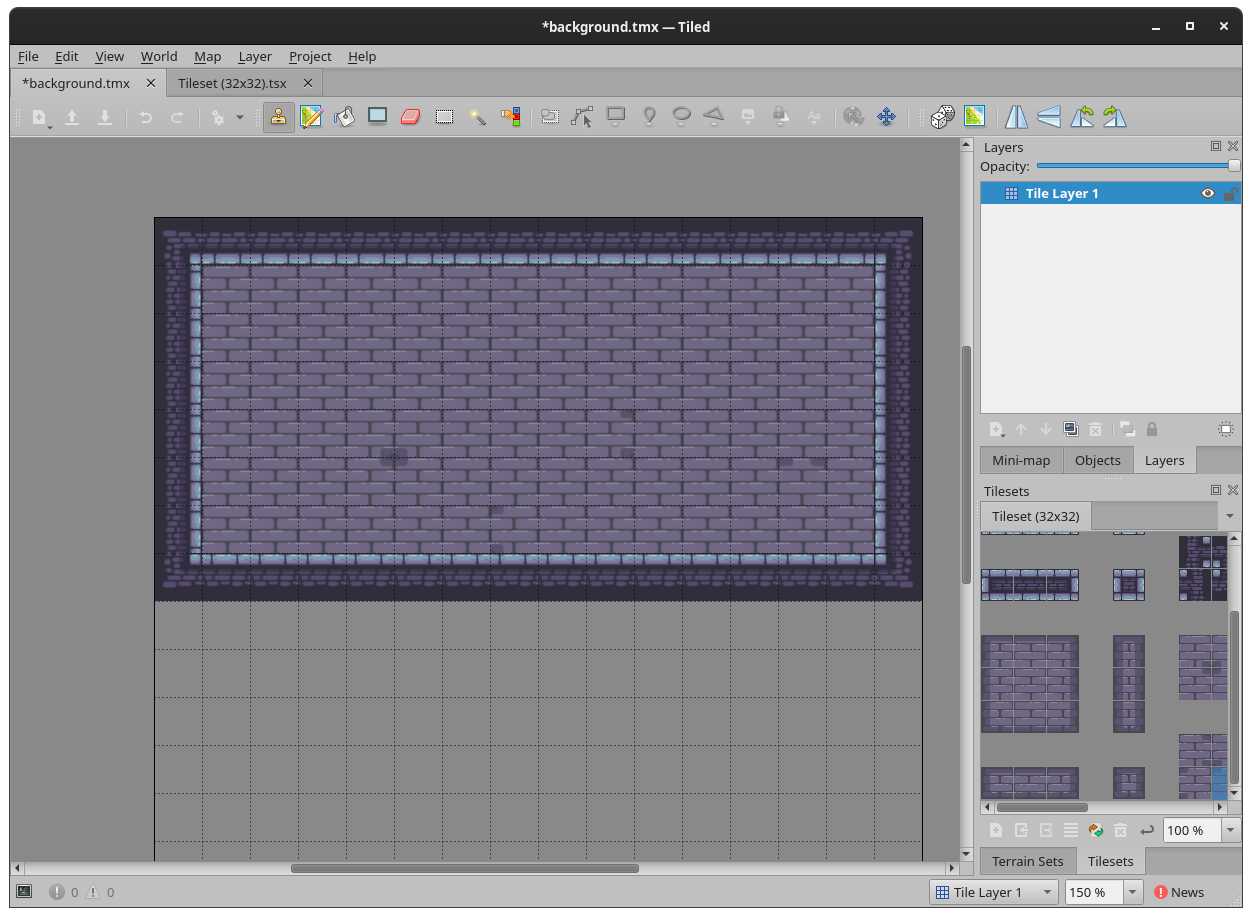
\includegraphics[width=.6\textwidth]{capitulos/capitulo3/tiled_demo_3.png}
	\caption{Creación de un fondo a partir del \textit{tileset}.}
	\label{fig:tiled_demo_3}
\end{figure}
\FloatBarrier

Esta metodología facilita la reutilización de recursos. No obstante, utilizar esta técnica requiere crear una tabla de índices adicional (o mapa) para poder especificar qué \textit{tile} se está utilizando \cite{bib:tonc}.

La reutilización se hace evidente si se consulta de nuevo la Figura~\ref{fig:tiled_demo_3} y se intenta identificar el número total de \textit{tiles} utilizados. En dicha Figura se utilizan 16 \textit{tiles} diferentes. En el caso de la Game Boy Advance este número se reduciría a 9, ya que en la tabla o mapa se puede especificar la orientación (invertir el eje horizontal o vertical) del \textit{tile}. La Figura~\ref{fig:tiled_demo_4} muestra el fondo junto con el índice de cada \textit{tile}.

\begin{figure}[h]
	\centering
	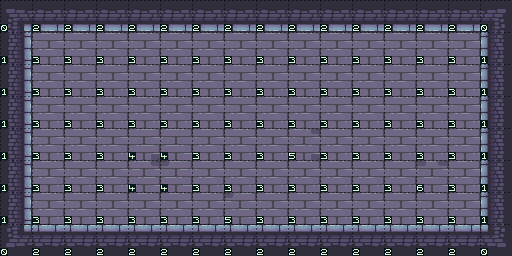
\includegraphics[width=.8\textwidth]{capitulos/capitulo3/tiled_demo_4.png}
	\caption{Distintos \textit{tiles} utilizados.}
	\label{fig:tiled_demo_4}
\end{figure}

En varias de las funciones que ofrece la \textit{PPU} es necesario especificar el posicionamiento de los \textit{tiles} a utilizar para poder renderizar la imagen correctamente. Es por esto que los \textit{tiles} se distribuyen en 32 grupos de 2048 bytes cada uno (conocidos como ``screenblocks'' en \cite{bib:tonc}). Estos grupos, a su vez, se organizan en 4 bloques todavía más abstractos de 16 KB cada uno (conocidos como ``charblocks'' en \cite{bib:tonc}). La distribución de los grupos descritos anteriormente sobre la VRAM se puede observar en la Tabla~\ref{tab:dist_charblocks}.

\begin{table}[h]
	\centering
	\begin{tabular}{| c | c | c | c | c |}
		\hline
		\textbf{Memoria} & 0x06000000 & 0x06004000 & 0x06008000 & 0x0600C000 \\ \hline
		``charblock'' & 0 & 1 & 2 & 3 \\ \hline
		``screenblock'' & \{0-7\} & \{8-15\} & \{16-23\} & \{24-31\} \\ \hline
	\end{tabular}
	\caption[Distribución de los \textit{tiles} en la VRAM.]{Distribución de los \textit{tiles} en la VRAM~\cite{bib:tonc}.}
	\label{tab:dist_charblocks}
\end{table}
\FloatBarrier{}

Para poder programar para el dispositivo, es necesario conocer también cómo trabaja la Game Boy Advance al posicionar píxeles y objetos en pantalla, además de cómo y cuándo se refresca la imagen.

Como se puede deducir de la distribución utilizada para los \textit{tiles}, la Game Boy Advance trata a la imagen como una matriz cuyas filas conforman el eje Y y las columnas el eje X. El punto de partida para los ejes, en el que su valor es 0, se posiciona en la esquina superior izquierda de la pantalla (véase la Figura~\ref{fig:y_x}).  Esto será de utilidad no solo en los modos \textit{bitmap} donde el programador manipulará la imagen a nivel de píxeles, sino también al trabajar con objetos y fondos, dado que será necesario indicar unas coordenadas para moverlos y posicionarlos.

\begin{figure}[h]
	\centering
	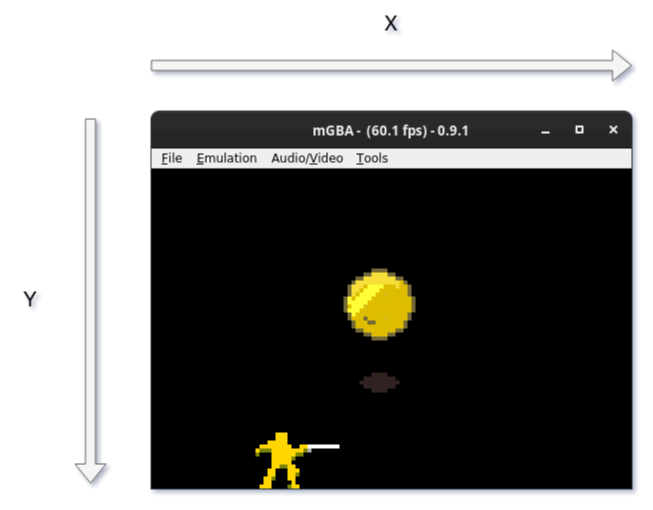
\includegraphics[width=.7\textwidth]{capitulos/capitulo3/y_x.png}
	\caption{Coordenadas de la pantalla.}
	\label{fig:y_x}
\end{figure}
\FloatBarrier

Al contrario de lo que pueda parecer, la forma en la que la pantalla de la Game Boy Advance se refresca influye en la manera en la que se programa para el dispositivo. Cada fotograma nuevo es actualizado no de ``golpe'', sino línea a línea (cada una de estas líneas recibe el nombre de \textit{scanline}). Entre cada línea refrescada existe un período llamado HBlank, y entre cada imagen refrescada existe un período llamado VBlank. Ambos ofrecen al programador un rango de tiempo en el que modificar ciertos parámetros sin distorsionar la imagen\footnote{En el caso de HBlank, esto no es del todo cierto en todos los casos dado que si se actualiza un \textit{sprite} durate HBlank es posible que se vea distorsionado.}. En total, la GBA cuenta con 228 \textit{scanlines} (el número de píxeles verticales más 68) de una longitud de 308 (el número de píxeles horizontales más 68). La Figura~\ref{fig:vblank_hblank} muestra los conceptos comentados anteriormente.

\begin{figure}[h]
	\centering
	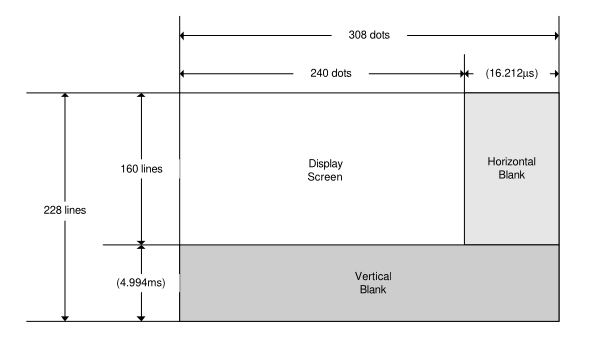
\includegraphics[width=.7\textwidth]{capitulos/capitulo3/lcd.png}
	\caption{Los períodos HBlank y VBlank en la pantalla de la GBA\@. Imagen de~\cite{bib:gba_manual}.}
	\label{fig:vblank_hblank}
\end{figure}
\FloatBarrier

Finalmente, queda mencionar que la consola utiliza un formato de 15 bits para representar colores. La distribución del rojo, verde y azul en este formato aparece representada en la Tabla~\ref{tab:15bit_color}. Como puede observarse, el bit más significativo no se usa \cite{bib:gba_manual}.

\begin{table}[h]
	\centering
	\begin{tabular}{| l | l | l | l | l | l | l | l | l | l | l | l | l | l | l | l |}
		\hline
		\o  & B & B & B & B & B & G & G & G & G & G & R & R & R & R & R \\ \hline
	\end{tabular}
	\caption{Color de 15 bits.}
	\label{tab:15bit_color}
\end{table}

Partiendo de los conceptos previos, se comentará a continuación el uso y funcionamiento de los mismos aplicados a los \textit{sprites}, fondos y \textit{bitmaps} de la Game Boy Advance.

\subsection{\textit{Sprites}}\label{sec:sprites}
La Game Boy Advance implementa a nivel de hardware un modo para manejar y mostrar personajes u objetos dentro del juego. \textit{Sprite} es el término que normalmente se utiliza para describir cualquier entidad única que se pueda mover dentro de un juego. El programador define los parámetros correspondientes y la \textit{PPU} se encargará de mostrar la imagen con los \textit{tiles} y colores que el programador haya posicionado en la VRAM y RAM de paleta, respectivamente. 

Por suerte para el programador, las tareas que se pueden considerar ``complejas'' las realiza la \textit{PPU} (por ejemplo, organizar los \textit{tiles}, tener en cuenta los bits por píxel y mostrarlos por pantalla). Aún así, tendrá que realizar los siguientes pasos para acabar mostrando el \textit{sprite} deseado:

\begin{enumerate}
	\item Separar los colores utilizados en una imagen, como un personaje o un objeto dentro del juego. Como resultado obtendremos una imagen con los índices apuntando a la paleta de colores.
	\item Dividir la imagen en bloques de 8x8, que es el tamaño base con el que trabaja la Game Boy Advance. Es en este punto donde se hace evidente la utilidad de herramientas como Grit, que automatiza la mayor parte de este proceso.
	\item Especificar las propiedades que tendrá el sprite en la OAM. Para ello, previamente, se han tenido que copiar los colores utilizados al espacio de memoria reservado para la paleta de colores y la distribución de los \textit{tiles} (los índices) a la VRAM.  Cada objeto almacenado en este espacio de memoria, que soporta hasta 128 \textit{sprites}, cuenta con tres atributos de 16 bits para definir sus propiedades.
	\item Indicar los valores que tendrán las matrices de transformación de 2x2 que se usen para rotar y escalar los \textit{sprites}. Este punto es opcional y se detallará más en profundidad en el apartado~\ref{sec:aff_obj}).
\end{enumerate}

La distribución de cada uno de estos atributos, junto con los valores de la matriz de transformación, siguen el formato expuesto en la Figura~\ref{fig:oam_dist} \cite{bib:tonc}. En dicha figura se utiliza $p$ para denotar al personaje u objeto, $Attr$ para cada uno de sus atributos y $a$ para referirse a los valores de la matriz. Es necesario recalcar que, mientras que la información de un \textit{sprite} es almacenada de forma contigua, los valores de la matriz de afinidad se encuentran dispersos, con 6 bytes de diferencia entre cada uno.

\begin{figure}[h]
	\centering
	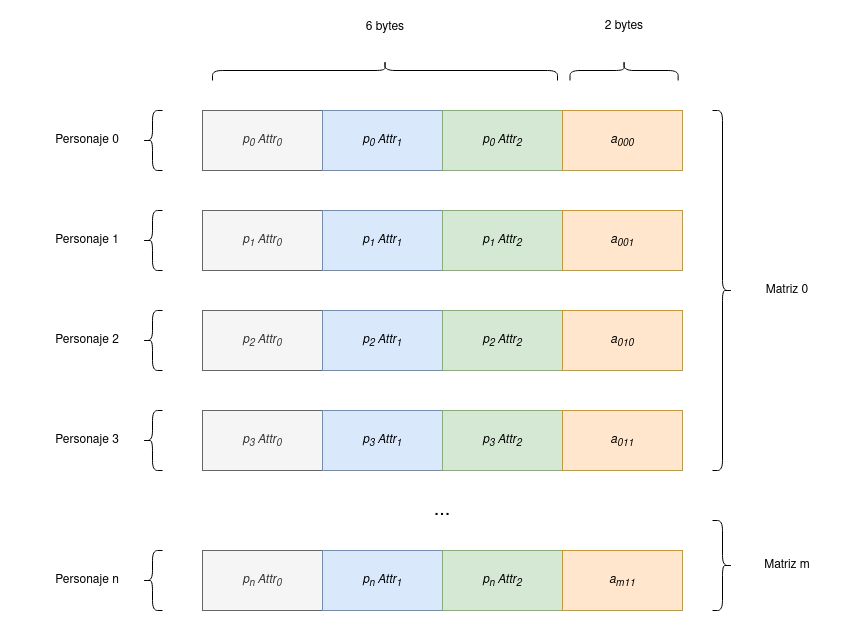
\includegraphics[height=10cm]{capitulos/capitulo3/oam_dist.png}
	\caption{Distribución de los atributos en la OAM.}
	\label{fig:oam_dist}
\end{figure}
\FloatBarrier{}

\subsubsection{Atributos}
Como se ha mencionado, las propiedades de los sprites se definen mediante tres atributos conocidos como 0, 1 y 2, que se explican a continuación. No obstante, para más información se recomienda consultar \cite{bib:gba_manual,bib:tonc}. Además, para las funciones que se puedan apreciar visualmente, se incluye un ejemplo mostrando su funcionamiento en esta sección y en la~\ref{sec:efectos}.

\vspace{1cm}
\underline{Atributo 0} \\ \\
Este atributo alberga las siguientes propiedades:

\begin{itemize}
	\item Bits \{F-E\}: Junto con los bits \{F-E\} del atributo 1, definen el tamaño de la imagen del objeto o personaje. Los tamaños posibles se pueden ver en la Tabla~\ref{tab:size}.

		\begin{table}[h]
			\centering
			\begin{tabular}{| l | l | l | l | l |}
				\hline
				\textbf{Atr. 0{\textbackslash}1} & \textbf{0} & \textbf{1} & \textbf{2} & \textbf{3}  \\ \hline
				\textbf{0} & 8x8 & 16x16 & 32x32 & 64x64  \\ \hline
				\textbf{1} & 16x8 & 32x8 & 32x16 & 64x32  \\ \hline
				\textbf{2} & 8x16 & 8x32 & 16x32 & 32x64  \\ \hline
			\end{tabular}
			\caption{Tamaño del \textit{sprite} según los valores de \{F-E\} en los atributos 0 y 1.}
			\label{tab:size}
		\end{table}
		\FloatBarrier

	\item Bit \{D\}: Bits por píxel. Este valor hay que ajustarlo dependiendo de la cantidad de colores que utilicen los \textit{tiles}. Si se iguala a 0, se utilizarán 4 bpp (bits por píxel), admitiendo una selección de 16 colores diferentes. En caso de igualarlo a 1, se utilizarán 8 bpp, ofreciendo una selección considerablemente mayor, con 256 colores diferentes. La desventaja es que cada \textit{tile} ocupará más espacio y, por lo tanto, habrá menos disponibles.
	\item Bit \{C\}: Bit de activación del efecto ``mosaico''. Este es uno de los efectos gráficos que ofrece la \textit{PPU} de la consola. Su función es ``pixelar'' todavía más el \textit{sprite} (o fondo, como se verá más adelante) en cuestión. Para utilizarlo es necesario activar este bit además de configurar el registro mostrado en la sección~\ref{sec:dispcnt}. Para más información consultar~\ref{sec:efectos_mosaico}.
	\item Bits \{B-A\}: Efectos adicionales. Están disponibles el \textit{blending} (que se consigue igualando este parámetro a 1) y el renderizado de máscara (que se consigue igualando este parámetro a 2). En caso de no especificar ningún valor (0), la \textit{PPU} renderizará el \textit{sprite} de forma normal.

		El primer modo, como su nombre sugiere, mezcla el \textit{sprite} (o fondo) con cualquier cosa que se encuentre detrás. El nivel de transparencia dependerá de los valores que se utilicen en los tres registros que usa, que se detallan posteriormente.

		El segundo no mostrará el \textit{sprite}, pero su área será utilizada para controlar cuales de los objetos o fondos que se encuentran dentro se renderizan.

	\item Bits \{9-8\}: En estos 2 bits, el programador podrá configurar cómo renderizar el \textit{sprite}. En concreto, si el objeto se rotará o cambiará de tamaño (igualando su valor a 1 o 3, respectivamente), si se ocultará (igualando a 2) o si su representación será la básica (igualando a 0), mostrando el objeto sin ningún cambio adicional. \\ \\
		Hay que resaltar que, dado que la Game Boy Advance inicializa la memoria a 0, el programador tendrá que asegurarse de que este parámetro sea 2 para todos los objetos no usados, aunque no utilice los 128 sprites disponibles. En caso contrario, en la esquina superior izquierda se mostrará el primer tile encontrado en la VRAM. Este problema se ilustra en la Figura~\ref{fig:artefacto}.

		\begin{figure}[h]
			\centering
			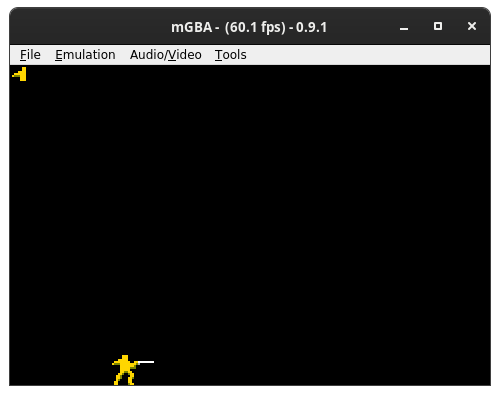
\includegraphics[width=.5\textwidth]{capitulos/capitulo3/artefacto.png}
			\caption{Resultado de no ocultar los \textit{sprites} no utilizados.}
			\label{fig:artefacto}
		\end{figure}
		\FloatBarrier

	\item Bits \{7-0\}: Las coordenadas Y del objeto siguiendo el formato especificado en la Figura~\ref{fig:y_x}.
\end{itemize}

La vista general de lo descrito anteriormente se puede observar en la Tabla~\ref{tab:sprite_attr0}. Para modificar las propiedades del atributo, el programador tiene que utilizar operadores a nivel de bit.

\begin{table}[h]
	\centering
	\begin{tabular}{| l | l |}
		\hline
		\textbf{Bits} & \textbf{Descripción} \\ \hline
		F-E & Tamaño del \textit{sprite}. \\ \hline
		D & Color utilizado. 0 para 4 bpp y 1 para 8 bpp. \\ \hline
		C & Efecto mosaico. \\ \hline
		B-A & Efectos especiales. \\ \hline
		9-8 & Modo de afinidad del objeto. \\ \hline
		7-0 & Coordenada Y del objeto. \\ \hline
	\end{tabular}
	\caption{Atributo 0.}
	\label{tab:sprite_attr0}
\end{table}
\FloatBarrier{}

\underline{Atributo 1} \\ \\
El atributo 1 incluye parámetros para invertir horizontal y verticalmente el \textit{sprite}, y otros que complementan los vistos en el atributo 0. La distribución es la mostrada a continuación:

\begin{itemize}
	\item Bits \{F-E\}: Junto con los bits \{F-E\} del atributo 0, definen el tamaño de la imagen utilizada para representar el objeto o personaje. Véase la Tabla~\ref{tab:size}.
	\item Bits \{D-C\}: Estos dos bits permiten al programador invertir tanto horizontal como verticalmente la imagen utilizada para representar el \textit{sprite}. Este recurso favorece la reutilización de los \textit{tiles} del \textit{sprite}, haciendo posible al programador invertir el objeto o personaje sin tener que guardar en memoria la imagen invertida.
		En la Figura~\ref{fig:invert_sprite} se muestra el efecto de todos los posibles valores que puede tener este campo. El primer \textit{sprite} aparece representado en su forma original, con el valor 0. El segundo \textit{sprite} se muestra invertido horizontalmente, con el valor 1. El tercer \textit{sprite} aparece invertido verticalmente, con el valor 2. Finalmente, el cuarto \textit{sprite} se representa invertido tanto horizontal como verticalmente, con el valor 3.

		\begin{figure}[h]
			\centering
			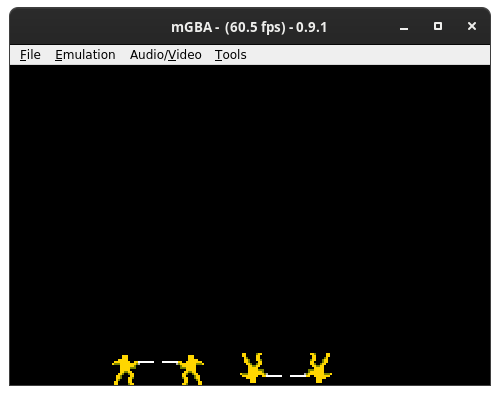
\includegraphics[width=.5\textwidth]{capitulos/capitulo3/invert_sprite.png}
			\caption{Demostración de los \textit{flags} para invertir un \textit{sprite} de diversas maneras.}
			\label{fig:invert_sprite}
		\end{figure}
		\FloatBarrier

	\item Bits \{D-9\}: En el caso de renderizar el \textit{sprite} a partir de una matriz, igualando el campo \{D-9\} del atributo 0 a 1, se especificará el índice de la matriz de afinidad a utilizar. Este valor no se podrá utilizar conjuntamente con los \textit{flags} de inversión mencionados anteriormente, dado que se superponen. No obstante, no es necesario teniendo en cuenta que se puede invertir mediante la matriz de transformación.
	\item Bits \{8-0\}: Define la coordenada X (se usará junto con la coordenada Y definida en el atributo 0).
\end{itemize}

La Tabla~\ref{tab:sprite_attr1} muestra, de manera resumida, los bits del atributo 1 junto con una breve descripción de su uso.

\begin{table}[h]
	\centering
	\begin{tabular}{| l | l |}
		\hline
		\textbf{Bits} & \textbf{Descripción} \\ \hline
		F-E & Tamaño del \textit{sprite}. \\ \hline
		D-C & \textit{Flags} para invertir el \textit{sprite}. \\ \hline
		D-9 & Índice de la matriz de transformación. \\ \hline
		8-0 & Coordenada X del objeto. \\ \hline
	\end{tabular}
	\caption{Atributo 1.}
	\label{tab:sprite_attr1}
\end{table}
\FloatBarrier{}

\underline{Atributo 2} \\ \\
El atributo 2 especifica parámetros relacionados con el renderizado de la imagen, como a partir de qué \textit{tile} se encuentra la imagen del objeto, la prioridad de renderizado y la paleta de colores a utilizar.

\begin{itemize}
	\item Bits \{F-C\}: Permiten indicar la paleta de colores a utilizar (el índice). Al igual que los \textit{flags} utilizados para invertir los \textit{sprites}, este es otro parámetro que puede ser de gran utilidad, dado que puede servir para generar personajes ``diferentes'' minimizando el uso de recursos. Un ejemplo de ello lo podemos ver en la Figura~\ref{fig:sprite_pal}.

		\begin{figure}[h]
			\centering
			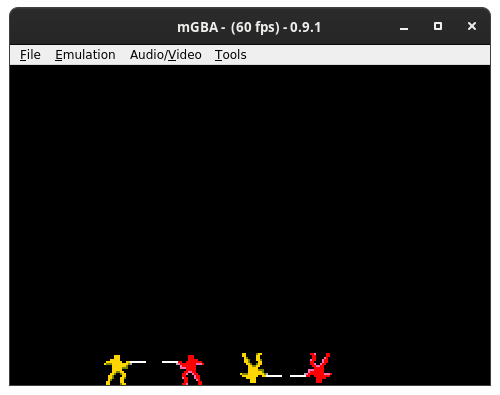
\includegraphics[width=.5\textwidth]{capitulos/capitulo3/sprite_pal.png}
			\caption{Utilizando los mismos \textit{tiles} se muestran diferentes \textit{sprites} alternando la paleta de colores de cada uno.}
			\label{fig:sprite_pal}
		\end{figure}
		\FloatBarrier

	\item Bits \{B-A\}: Este valor determina el orden con el que se renderizan los \textit{sprites} por pantalla. Cuanto mayor sea el número, antes se ``pintará'' y, por lo tanto, el objeto quedará en segundo plano al superponerse con otro de menor prioridad.
	\item Bits \{9-0\}: En estos 10 bits se especifica el primer \textit{tile} del objeto a ``pintar''. Dado que en parámetros previos se indican el tamaño de la imagen y los colores utilizados, la \textit{PPU} es capaz de saber cuántos \textit{tiles} tiene que procesar simplemente a partir del primer índice. Este valor no solo sirve para mostrar diferentes \textit{sprites} por pantalla, sino que facilita la realización las animaciones de \textit{sprites} al programador. Este solo tendría que cambiar dicho valor cada cierto tiempo.

\end{itemize}

La Tabla~\ref{tab:sprite_attr2} resume los bits utilizados, junto con una breve descripción, del atributo 2.

\begin{table}[h]
	\centering
	\begin{tabular}{| l | l |}
		\hline
		\textbf{Bits} & \textbf{Descripción} \\ \hline
		F-C & Especifica la paleta a utilizar. \\ \hline
		B-A & Prioridad de renderizado. \\ \hline
		9-0 & Índice del primer \textit{tile} del objeto. \\ \hline
	\end{tabular}
	\caption{Atributo 2.}
	\label{tab:sprite_attr2}
\end{table}


\subsubsection{Matriz de transformación}\label{sec:aff_obj}
Como se ha mencionado en los parámetros de los atributos 0 y 1, la PPU \textit{permite} al programador rotar, escalar y recortar el sprite mediante transformaciones afines. Este tipo de transformaciones, en el caso de la Game Boy Advance, se calculan con una matriz 2x2 al tratarse de un espacio 2D.

El concepto es relativamente simple. Se tiene un punto (o conjunto de puntos) definido por la ecuación \eqref{eq:eq_1} que se desea procesar. Para hacerlo, se multiplicará por la matriz de transformación, que tendrá la estructura descrita en la ecuación~\eqref{eq:eq_2}. Dependiendo de la operación que se quiera realizar, los valores $a_{00}, a_{01}, a_{10}$ y $a_{11}$ irán variando. El punto resultante, $p$, queda definido según la ecuación~\eqref{eq:eq_3}~\cite{bib:aff_matrix}:

\begin{align}
	p = 
	\begin{bmatrix}
		x\\
		y
	\end{bmatrix}
	\label{eq:eq_1}
\end{align}

\begin{align}
	A = 
	\begin{bmatrix}
		a_{00} & a_{01}\\
		a_{10} & a_{11}
	\end{bmatrix}
	\label{eq:eq_2}
\end{align}


El problema que complica ligeramente la situación al programador es que la GBA ``mapea'' los valores desde la pantalla a las texturas. Dado que el cálculo descrito en la ecuación~\eqref{eq:eq_3} es para convertir una coordenada del espacio de texturas a la pantalla, se tendrá que invertir la matriz de transformación para conseguir el resultado deseado \cite{bib:algebra}. La ecuación final quedaría como se puede observar en la ecuación~\eqref{eq:eq_4}.

\begin{align}
	p' = A  p
	\label{eq:eq_3}
\end{align}


\begin{align}
	p = A^{-1}  p'
	\label{eq:eq_4}
\end{align}

En cuanto al cálculo de la matriz inversa se refiere, al tratarse de una matriz 2x2, se puede utilizar la fórmula mostrada en~\eqref{eq:eq_5} siguiendo uno de los teoremas explicados en \cite{bib:algebra}. Aplicada a la ecuación~\eqref{eq:eq_2}, quedaría como se observa en la ecuación~\eqref{eq:eq_6}.

\begin{align}
	A^{-1} =
	\frac{1}{|A|}
	adj(A)^t
	\label{eq:eq_5}
\end{align}

\begin{align}
	\begin{bmatrix}
		a_{00} & a_{01}\\
		a_{10} & a_{11}
	\end{bmatrix}^{-1}
	=
	\frac{1}{a_{00}a_{11}-a_{01}a_{10}}
	\begin{bmatrix}
		a_{11} & -a_{01}\\
		-a_{10} & a_{00}
	\end{bmatrix}
	\label{eq:eq_6}
\end{align}

A continuación, se van a mostrar varios ejemplos junto con la matriz de transformación utilizada. Se omitirá la matriz de identidad al no modificar la imagen resultante.

Aprovechando que este recurso permite una mayor flexibilidad que los \textit{flags} de inversión del atributo 1, se probarán con ángulos que una simple inversión no puede proporcionar. El primero de ellos es un ángulo de 45º, cuya matriz, al ser de rotación, utiliza funciones coseno ($cos$) y seno ($sin$) \cite{bib:aff_matrix}. La matriz quedaría como se puede observar en la ecuación~\eqref{eq:eq_7}. Al hacer el cálculo, se obtiene que la matriz inversa es idéntica a la original.

\begin{align}
	A
	=
	A^{-1}
	=
	\begin{bmatrix}
		\cos(\theta) & -\sin(\theta)\\
		\sin(\theta) & \cos(\theta)
	\end{bmatrix}
	\label{eq:eq_7}
\end{align}
\newpage
La Figura~\ref{fig:rot_45} incluye el resultado de usar esta matriz con los ejemplos anteriores.

\begin{figure}[h]
	\centering
	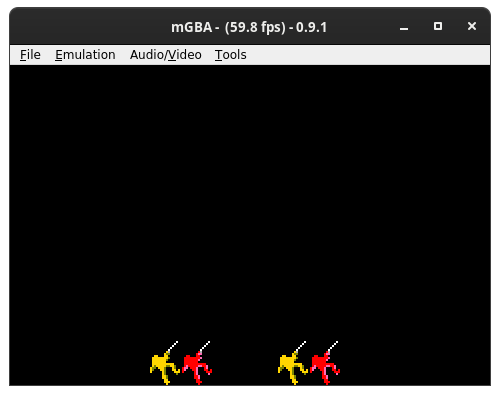
\includegraphics[width=.5\textwidth]{capitulos/capitulo3/rot_45.png}
	\caption{Rotación de \textit{sprites} por medio de la matriz de transformación.}
	\label{fig:rot_45}
\end{figure}
\FloatBarrier

Otra matriz utilizada a menudo es la de escalado. Como su nombre indica, permite aumentar el tamaño del \textit{sprite} tanto en el eje X como en el Y \cite{bib:aff_matrix}. La matriz utilizada en este ejemplo se muestra en la ecuación \eqref{eq:eq_7}, siendo $a$ el factor de escalado en el eje X y $d$ el factor de escalado en Y. La inversa quedaría como se muestra en la ecuación~\eqref{eq:eq_9}.

\begin{align}
	A
	=
	\begin{bmatrix}
		a & 0 \\
		0 & d
	\end{bmatrix}
	\qquad
\end{align}

\begin{align}
	A^{-1}
	=
	\begin{bmatrix}
		1/a & 0 \\
		0 & 1/d
	\end{bmatrix}
	\label{eq:eq_9}
\end{align}

El resultado de multiplicar por 2 tanto el eje X como Y en el programa de demostración es el que se muestra en la Figura~\ref{fig:scale_2}.

\begin{figure}[h]
	\centering
	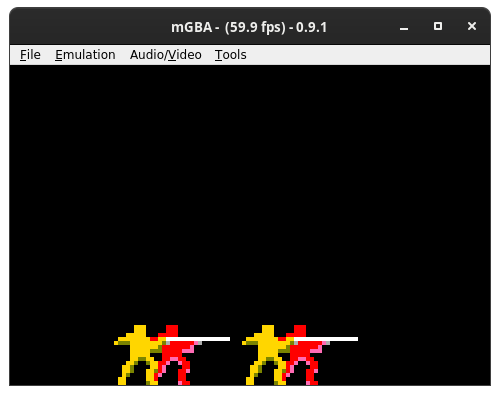
\includegraphics[width=.5\textwidth]{capitulos/capitulo3/scale_2.png}
	\caption{Escalado \textit{sprites} por medio de una matriz de transformación.}
	\label{fig:scale_2}
\end{figure}
\FloatBarrier{}

En caso de querer rotar y escalar el \textit{sprite} a la vez, esto se puede realizar combinando las fórmulas mostradas anteriormente (ecuaciones~\eqref{eq:eq_10} y~\eqref{eq:eq_11}), tal y como se muestra en la ecuación \eqref{eq:eq_12}.

\begin{align}
	A_e^{-1}
	=
	\begin{bmatrix}
		1/a & 0 \\
		0 & 1/d
	\end{bmatrix}
	\label{eq:eq_10}
\end{align}

\begin{align}
	A_r^{-1}
	=
	\begin{bmatrix}
		\cos(\theta) & -\sin(\theta)\\
		\sin(\theta) & \cos(\theta)
	\end{bmatrix}
	\label{eq:eq_11}
\end{align}

\begin{align}
	A_{re}^{-1}
	=
	\begin{bmatrix}
		1/a & 0 \\
		0 & 1/d
	\end{bmatrix}
	\begin{bmatrix}
		\cos(\theta) & -\sin(\theta)\\
		\sin(\theta) & \cos(\theta)
	\end{bmatrix}
	=
	\begin{bmatrix}
		\cos(\theta)/a & -\sin(\theta)/a\\
		\sin(\theta)/d & \cos(\theta)/d
	\end{bmatrix}
	\label{eq:eq_12}
\end{align}

Esto da lugar a la Figura~\ref{fig:scale_and_rot}, en la que se combina una rotación de 30º con un factor de escala de 1.5 en los dos ejes.

\begin{figure}[h]
	\centering
	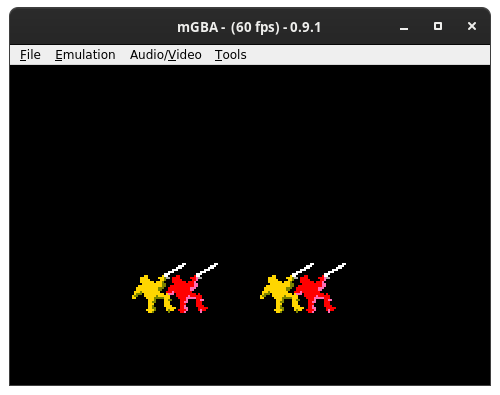
\includegraphics[width=.55\textwidth]{capitulos/capitulo3/rot_scale_30_1.5.png}
	\caption{Rotación y escalado de \textit{sprites} por medio de la matriz de transformación.}
	\label{fig:scale_and_rot}
\end{figure}
\FloatBarrier{}

Lamentablemente, este sistema trae consigo varias limitaciones y problemas. El primero de ellos es la imposibilidad de rotar, escalar y realizar transformaciones de corte si el \textit{sprite} resultante sobrepasa el área original establecida (el tamaño original del \textit{sprite}, véase la Tabla~\ref{tab:size}). Esto se puede resolver igualando el parámetro \{9-8\} del atributo 0 a 3, duplicando el área original del objeto. Sin embargo, si el \textit{sprite} sobrepasa esa área, también se verá cortado (véase la Figura~\ref{fig:too_big}). Además, el programador deberá tener en cuenta el cambio en las coordenadas X e Y al posicionar el \textit{sprite} en pantalla.


\begin{figure}[h]
	\centering
	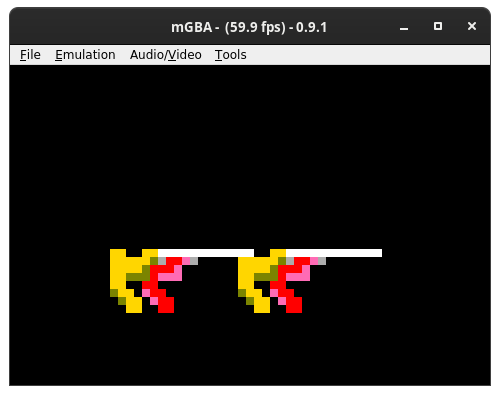
\includegraphics[width=.55\textwidth]{capitulos/capitulo3/too_big.png}
	\caption{\textit{Sprite} que sobrepasa el área permitida.}
	\label{fig:too_big}
\end{figure}
\FloatBarrier{}

La segunda limitación es el uso, en varios casos, de operaciones en punto flotante y funciones $cos$ y $sin$. El hecho de que la consola no cuente con una \textit{FPU} (\textit{Floating Point Unit}) ralentiza de manera considerable el cálculo. Por lo tanto, habrá que evitar este tipo de operaciones no solo al calcular la matriz de transformación, sino en otros aspectos del programa también. De hecho, el dispositivo no acepta \textit{floats} como valores de la matriz de transformación, solo permite números de coma fija (\textit{fixed point numbers} en inglés). El uso de este tipo de números se verá con más detenimiento en la Sección~\ref{sec:aspectos}.

\subsection{Bitmaps}\label{sec:bitmaps}
A diferencia de sus predecesoras, la Game Boy Advance proporciona al programador una forma directa de manipular los píxeles que aparecen por pantalla, lo que se conoce como \textit{bitmap}. Este modo, considerado como el más simple de los que ofrece el dispositivo, trata el contenido de la sección de memoria VRAM como los píxeles de la pantalla. Por lo tanto, con escribir en esta dirección de memoria, la pantalla inmediatamente representará los cambios reflejados sin tener que cambiar o configurar ningún registro o atributo adicional.

Este modo no es del todo práctico ni eficiente, dado que se tiene que suministrar el valor de cada uno de los píxeles que aparecen por pantalla. Sin embargo, sigue siendo válido para mostrar imágenes estáticas, realizar juegos relativamente simples (como \textit{Pong}) o 3D como \textit{Doom}\footnote{\url{https://doom.fandom.com/wiki/Game_Boy_Advance}}.

Concretamente, existen tres modos \textit{bitmap} para manipular directamente los píxeles. Se diferencian en aspectos como el tamaño del \textit{canvas}, si se recurre a una paleta de colores o si se cuenta con un buffer adicional  \cite{bib:gba_manual}.

La Tabla~\ref{tab:modos_bitmap} resume las diferencias principales de los modos, de los que se dan más detalles en las siguientes subsecciones.

\begin{table}[h]
	\centering
	\begin{tabular}{| l | l | l | l | l | l |}
		\hline
		\textbf{Modo} & \textbf{Ancho} & \textbf{Alto} & \textbf{bpp} & \textbf{Uso de paleta} & \textbf{Buffer adicional} \\ \hline
		3 & 240 & 160 & 16 & No & No \\ \hline
		4 & 240 & 160 & 8 & Sí & Sí \\ \hline
		5 & 160 & 128 & 16 & No & Sí \\ \hline
	\end{tabular}
	\caption{Modos bitmap de la Game Boy Advance. Tabla basada en \cite{bib:tonc}}
	\label{tab:modos_bitmap}
\end{table}
\FloatBarrier{}

\subsubsection{Modo 3}\label{sec:mode_3}
El modo 3 ofrece al programador un buffer de 240x160 de 16 bits por píxel, resolución que coincide con la pantalla de la Game Boy Advance. De los 16 bits, se utilizan 15 para cada color como se mostró en la Tabla~\ref{tab:15bit_color}. En total, este buffer ocupa 75 KB, desde la dirección 0x06000000 (VRAM) \cite{bib:gba_manual}.

\begin{figure}[h]
	\centering
	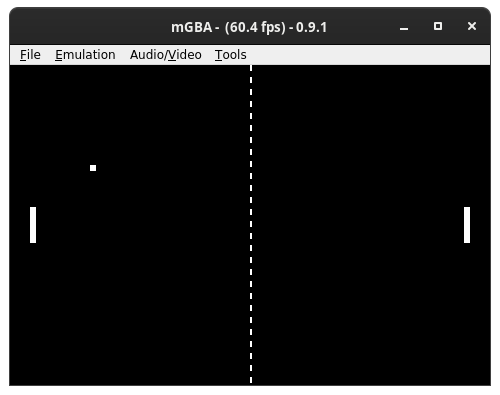
\includegraphics[width=.55\textwidth]{capitulos/capitulo3/bitmaps_3.png}
	\caption{Demostración práctica del uso del Modo 3.}
	\label{fig:modo_3}
\end{figure}
\FloatBarrier

En la Figura~\ref{fig:modo_3} se puede observar un ejemplo de un juego simple que utiliza el modo 3 de la \textit{PPU}.

Como dato adicional, es posible utilizar conjuntamente los modos \textit{bitmaps} y el modo de \textit{sprites}. Sin embargo, en el caso del modo 3 se disminuye el espacio destinado a \textit{tiles} un 50\% \cite{bib:tonc}.

\subsubsection{Modo 4}\label{sec:mode_4}
El modo 4, a pesar de utilizar un \textit{canvas} idéntico al modo 3, de 240x160 también, incluye varias opciones interesantes para el programador.

Para empezar, en lugar de guardar los valores de los píxeles directamente en la VRAM, guarda los índices de la paleta de colores que se encuentra en la RAM de paleta. A la hora de modificar el color de una gran cantidad de píxeles, esto puede suponer una ventaja en términos de rendimiento con respecto al modo 3. Dada la inherente ineficiencia que supone modificar cada uno de los píxeles que aparecen por pantalla, tener índices apuntando a una paleta de colores permite al programador cambiar un gran número de píxeles simplemente cambiando uno de los valores de la paleta.

Además, al utilizar índices, que ocupan 8 bits, el espacio dedicado a la imagen se reduce a la mitad. Este espacio ``extra'' lo aprovecha un buffer que ofrece el modo 4. Este buffer adicional se encuentra en la dirección de memoria 0x0600A000. El buffer principal del modo 4 acaba en 0x06009600, por lo que no interfiere con el segundo buffer disponible. La idea es que el programador escriba el próximo ``frame'' en el buffer no activo para posteriormente modificar el buffer activo. Así se consigue que los cambios realizados no hagan que la imagen final sufra \textit{tearing}, es decir, que no se superpongan imágenes de forma indebida~\cite{bib:gba_manual,bib:tonc}.

\subsubsection{Modo 5}\label{sec:mode_5}
El modo 5 ofrece tanto la posibilidad de escribir directamente en VRAM sin tener que utilizar una paleta con color de 15 bits, como un segundo buffer donde preparar el siguiente frame. Aunque, en detrimento del jugador, usa un canvas de dimensiones reducidas, de 160x128 \cite{bib:gba_manual}. La Figura~\ref{fig:modo_5} da una idea al lector del área que abarca este modo.

\begin{figure}[h]
	\centering
	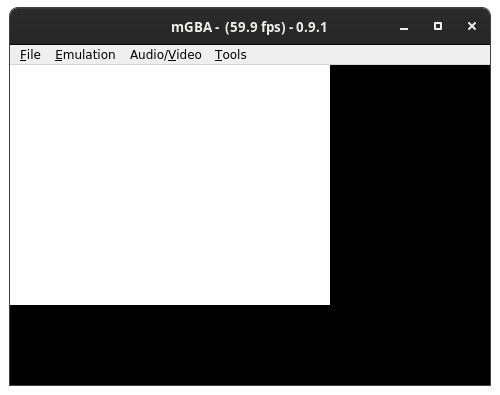
\includegraphics[width=.55\textwidth]{capitulos/capitulo3/bitmaps_5.png}
	\caption{Ejemplo práctico del modo 5.}
	\label{fig:modo_5}
\end{figure}
\FloatBarrier

Al igual que el modo 3, el modo 5 usa gran parte de la VRAM, lo que reduce el número de \textit{tiles} disponibles para \textit{sprites} \cite{bib:tonc}.

\subsection{Fondos}\label{sec:fondos}
Los fondos de la GBA permiten especificar mediante el uso de ``mapas'' qué \textit{tiles} utilizar para rellenar el canvas. A pesar de que técnicamente los \textit{bitmaps} se catalogan como fondos en el manual \cite{bib:gba_manual}, se suelen separar los modos 0, 1, 2 y 3 de los modos 4, 5 y 6 por las grandes diferencias de funcionamiento.

A diferencia de los \textit{sprites}, la mayor parte de la configuración se hace en los registros de configuración específicos para los fondos. Por lo tanto, lo que hay que tener en cuenta al mostrar fondos en la consola es el formato que sigue cada una de las entradas del mapa, que especifica el \textit{tile} a utilizar y el número y tipo de fondos a emplear.

En cuanto al formato que sigue una entrada del mapa correspondiente a un fondo, tiene la siguiente distribución:

\begin{itemize}
	\item Bits \{F-C\}: Índice de la paleta de colores a utilizar en caso de estar en el modo de color de 4 bpp.
	\item Bits \{B-A\}: Es similar a lo visto en el atributo 1 de los \textit{sprites}. Permite invertir tanto horizontal como verticalmente el \textit{tile} especificado en los bits \{9-0\}.
	\item Bits \{9-0\}: Índice del \textit{tile} a utilizar.
\end{itemize}

Sin embargo, con las herramientas disponibles, el programador no tendrá que preocuparse del formato que sigue cada entrada en el mapa. Las utilidades como Grit ya automatizan la generación de los mapas de cada fondo.

Lo que si tiene que tener en cuenta el programador son los modos que configurará en los registros mostrados en la sección~\ref{sec:conf_fondos}, indicando cuántos de los 4 fondos disponibles planea utilizar y si utilizarán una matriz de transformación. Dependiendo de los modos seleccionados, unos fondos u otros quedarán inhabilitados o limitados a un uso específico. En la Tabla~\ref{tab:modos_fondos} se denota con ``r'' a los fondos normales y con ``t'' a los fondos que utilizan la matriz de transformación.

\begin{table}[h]
	\centering
	\begin{tabular}{| l | l | l | l | l |}
		\hline
		\textbf{Modo} & \textbf{Fondo 0} & \textbf{Fondo 1} & \textbf{Fondo 2} & \textbf{Fondo 3} \\ \hline
		0 & r & r & r & r \\ \hline
		1 & r & r & t  & - \\ \hline
		2 & - & - & t & t \\ \hline
	\end{tabular}
	\caption{Modos para los fondos de la Game Boy Advance.}
	\label{tab:modos_fondos}
\end{table}

Otro aspecto que se ve afectado por el modo seleccionado es el tamaño del fondo. Tal y como se puede observar en la Tabla~\ref{tab:size_bg}, el tamaño del fondo depende en parte de si utiliza una matriz de transformación. El valor de la columna \textit{flag} es el que le corresponde a los bits \{F-E\} en el registro de control. Los valores mostrados utilizan como base el \textit{tile} de 8x8 y, para dar una mejor idea del tamaño, se incluye entre paréntesis el tamaño en píxeles del fondo.

\begin{table}[h]
	\centering
	\begin{tabular}{| l | l | l |}
		\hline
		\textbf{Flag} & \textbf{Tamaño para \textit{r}} & \textbf{Tamaño para \textit{t}} \\ \hline
		00 & 32x32 (256x256) & 16x16 (128x128) \\ \hline
		01 & 64x32 (512x256) & 32x32 (256x256) \\ \hline
		10 & 32x64 (256x512) & 64x64 (512x512) \\ \hline
		11 & 64x64 (512x512) & 128x128 (1024x1024) \\ \hline
	\end{tabular}
	\caption{Tamaños disponibles para cada uno de los fondos.}
	\label{tab:size_bg}
\end{table}
\FloatBarrier{}

Una demostración de un fondo renderizado se puede observar en la Figura~\ref{fig:fondo_1}. Se trata de un fondo de 32x32 (o 256x256 píxeles) en movimiento actualizando los valores de los registros de offset.

\begin{figure}[h]
     \centering
         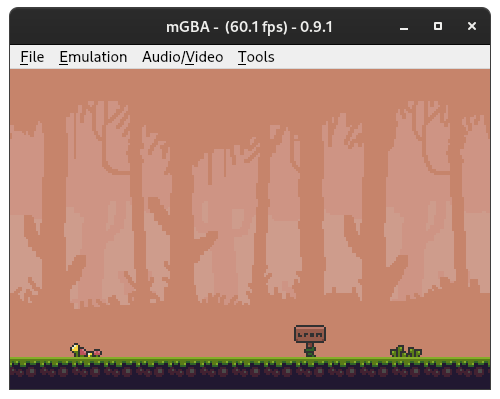
\includegraphics[width=.55\textwidth]{capitulos/capitulo3/fondo_1.png}
	\caption{Fondo 32x32.}\label{fig:fondo_1}
\end{figure}
\FloatBarrier{}

Además de las diferencias de tamaño observadas en la Tabla~\ref{tab:size_bg}, los fondos que utilizan la matriz de transformación también ven las entradas del mapa modificadas. En este caso se prescinde del índice de paleta y de la orientación de cada \textit{tile}. De esta forma, cada entrada del mapa acaba siendo solo el índice del mapa y su tamaño se ve reducido a 1 byte \cite{bib:tonc}.

Basándose en los mismos conceptos vistos en la sección~\ref{sec:aff_obj}, hay que definir los valores de una matriz 2x2 para modificar el fondo en cuestión. En la Figura~\ref{fig:fondos_aff} se ofrecen dos variantes del fondo mostrado en la Figura~\ref{fig:fondo_2} cambiando el tamaño y la rotación del mismo.

\begin{figure}[h]
     \centering
         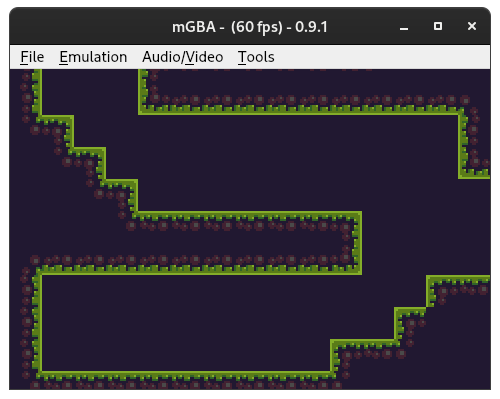
\includegraphics[width=.55\textwidth]{capitulos/capitulo3/affine_bg_1.png}
	\caption{Fondo 32x32.}\label{fig:fondo_2}
\end{figure}
\FloatBarrier{}

\begin{figure}[h]
     \centering
     \begin{subfigure}[b]{0.45\textwidth}
         \centering
         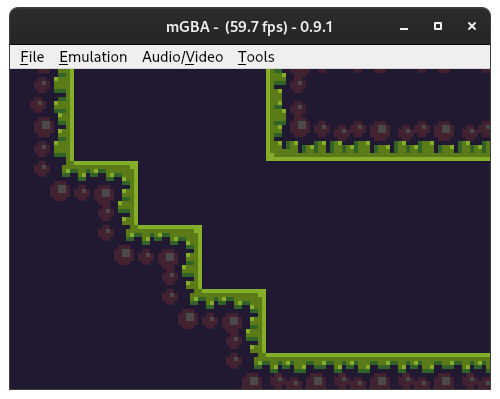
\includegraphics[width=\textwidth]{capitulos/capitulo3/affine_bg_2.png}
         \label{fig:fondo_3}
	     \caption{Fondo escalado un 100\%.}
     \end{subfigure}
     \hfill
     \begin{subfigure}[b]{0.45\textwidth}
         \centering
         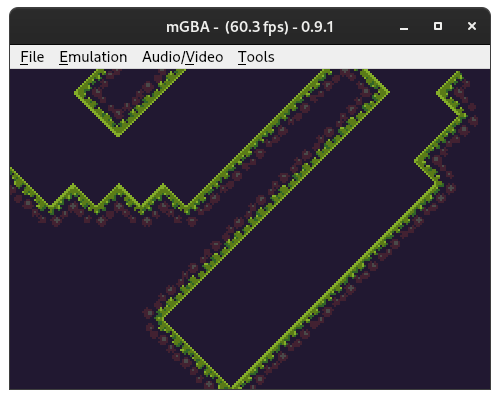
\includegraphics[width=\textwidth]{capitulos/capitulo3/affine_bg_3.png}
         \label{fig:fondo_4}
	     \caption{Fondo rotado por 45º.}
     \end{subfigure}
	\caption{Matriz de transformación sobre el fondo de la Figura~\ref{fig:fondo_2}.}\label{fig:fondos_aff}
\end{figure}
\FloatBarrier{}

\subsection{Efectos especiales}\label{sec:efectos}
La GBA ofrece al programador diversas formas de pulir y refinar sus juegos con efectos especiales acelerados por hardware. Los cuatro efectos especiales son el \textbf{\textit{blending}}, \textbf{efectos \textit{fade in/out}}, el \textbf{modo ``mosaico''} y el \textbf{modo ventana}.

Todos ellos se pueden aplicar tanto a \textit{sprites} como a fondos. El efecto no varía si se aplica a un objeto o a un fondo, por lo que los ejemplos mostrados valen para ambos.

\subsubsection{\textit{Blending}}\label{sec:efectos_blending}
Como su nombre sugiere, permite mezclar los colores que se encuentran detrás del \textit{sprite}, ya sea un fondo u otro \textit{sprite}. El nivel del efecto se configura en los registros adicionales vistos en el sección~\ref{sec:dispcnt}.

El registro que guarda los coeficientes de mezcla, BLDALPHA (para más información consultar el sección~\ref{sec:dispcnt}), calcula el valor de cada píxel siguiendo la fórmula mostrada en la ecuación~\eqref{eq:blending}. El cálculo se realiza para cada color de forma separada, de ahí el mínimo de 31, número que representa el máximo valor que puede alcanzar un color de 5 bits.

\begin{align}
	valor
	=
	min(31, color_{frontal} * coef_{frontal} + color_{posterior} * coef_{posterior})	
	\label{eq:blending}
\end{align}

Una demostración del efecto que se consigue con el \textit{sprite} utilizado anteriormente combinado con un fondo gris se puede observar en la Figura~\ref{fig:blending}.

\begin{figure}[h]
     \centering
     \begin{subfigure}[b]{0.45\textwidth}
         \centering
         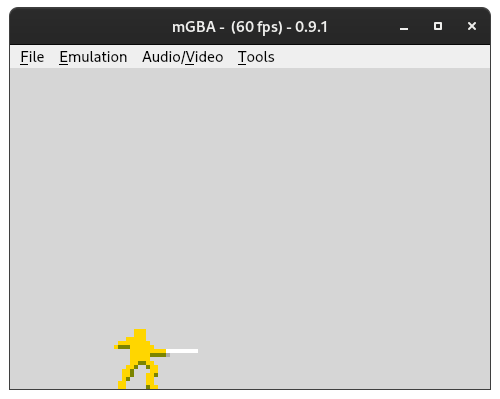
\includegraphics[width=\textwidth]{capitulos/capitulo3/blending_1.png}
         \label{fig:blending_1}
	     \caption{Demostración sin \textit{blending}.}
     \end{subfigure}
     \hfill
     \begin{subfigure}[b]{0.45\textwidth}
         \centering
         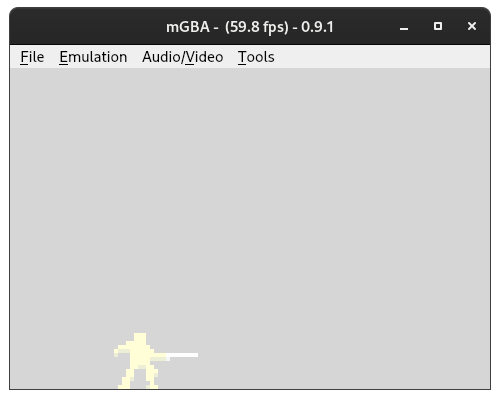
\includegraphics[width=\textwidth]{capitulos/capitulo3/blending_2.png}
         \label{fig:blending_2}
	     \caption{Demostración con \textit{blending}.}
     \end{subfigure}
	\caption{Efecto conseguido configurando el efecto \textit{blending} de la consola.}\label{fig:blending}
\end{figure}
\FloatBarrier{}

\subsubsection{Efectos \textit{fade}}\label{sec:efectos_fade}
Para facilitar las transiciones entre escenas, la \textit{PPU} ofrece la posibilidad de cambiar gradualmente de una imagen a otra completamente negra, y de una imagen a otra completamente blanca. 

Configurando los registros BLDCNT y BLDY vistos en la sección~\ref{sec:dispcnt}, se modifica la intensidad de la imagen mostrada por pantalla. Si se actualiza el valor de BLDY se conseguirá el deseado efecto \textit{fade in/out}. En las Figura~\ref{fig:brightness} se muestra un aumento y disminución de la intensidad sobre una imagen. 

\begin{figure}[h]
     \centering
     \begin{subfigure}[b]{0.45\textwidth}
         \centering
         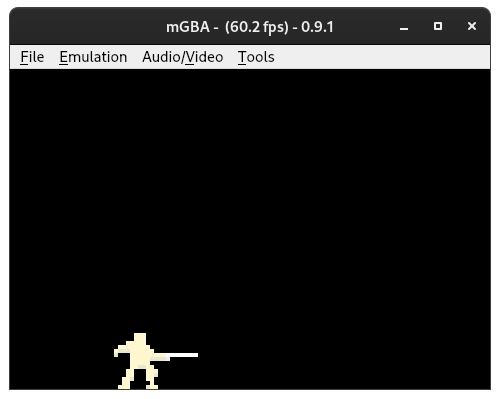
\includegraphics[width=\textwidth]{capitulos/capitulo3/brightness_3.png}
         \label{fig:blending_1}
	     \caption{Aumento de la intensidad.}
     \end{subfigure}
     \hfill
     \begin{subfigure}[b]{0.45\textwidth}
         \centering
         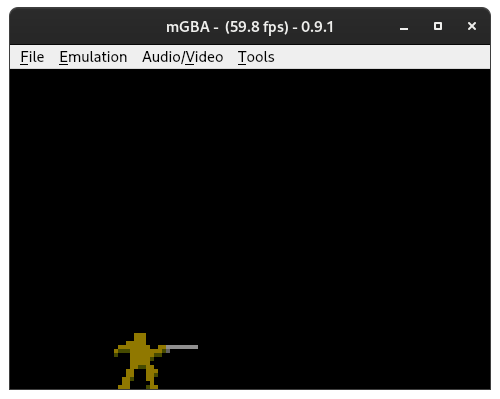
\includegraphics[width=\textwidth]{capitulos/capitulo3/brightness_4.png}
         \label{fig:blending_2}
	     \caption{Disminución de la intensidad.}
     \end{subfigure}
	\caption{Demostración del cambio de intensidad a través de BLDCNT y BLDY.}\label{fig:brightness}
\end{figure}
\FloatBarrier{}

\subsubsection{Modo mosaico}\label{sec:efectos_mosaico}
Este modo reduce el nivel de detalle de un objeto o fondo. Para ello, la GBA internamente aplica el valor de un píxel a los vecinos posicionados debajo y a su derecha. El número de píxeles que acaban compartiendo el mismo valor quedará determinado por el número de distorsión horizontal y vertical que se indique en el registro correspondiente. Por ejemplo, si el píxel 0 tiene un valor determinado y la distorsión horizontal es de 10, entonces los píxeles 1-10 tendrán el mismo color que el píxel 0. Siguiendo el ejemplo, si la distorsión horizontal es de 10, el siguiente píxel a tener en cuenta sería el 11.
Un ejemplo del efecto se puede observar en la Figura~\ref{fig:mosaic}.

		\begin{figure}[h]
			\centering
			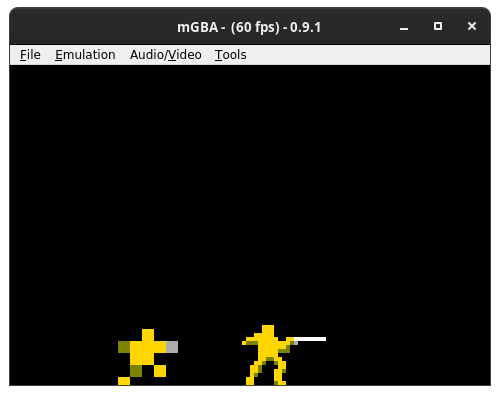
\includegraphics[width=.45\textwidth]{capitulos/capitulo3/mosaic.png}
			\caption{Sprite renderizado con efecto ``mosaico'' (izquierda), junto a su representación sin alterar (derecha).}
			\label{fig:mosaic}
		\end{figure}
		\FloatBarrier


\subsubsection{Modo ventana}\label{sec:efectos_ventana}
El último efecto destacable que ofrece la GBA es la posibilidad de crear ventanas en pantalla y controlar qué contenido es renderizado dentro y fuera de ellas. La consola proporciona 2 ventanas para fondos, y cada \textit{sprite} puede configurarse para controlar qué se renderiza dentro y fuera del área que ocupa. En caso de superponerse las dos ventanas disponibles, el contenido renderizado es la unión del contenido permitido en ambas. Por otra parte, el contenido no renderizado es todo lo que no entra en la unión mencionada anteriormente.

La Figura~\ref{fig:windows} muestra un ejemplo sobre el fondo de la Figura~\ref{fig:fondo_1}. En este ejemplo se observa una ventana que ocupa la mitad de la pantalla en la que se permite el renderizado de dos fondos (el fondo con el paisaje y el fondo con la vegetación). Fuera de la ventana, solo se permite el renderizado de uno de los fondos (el de la vegetación).

\begin{figure}[b]
	\centering
	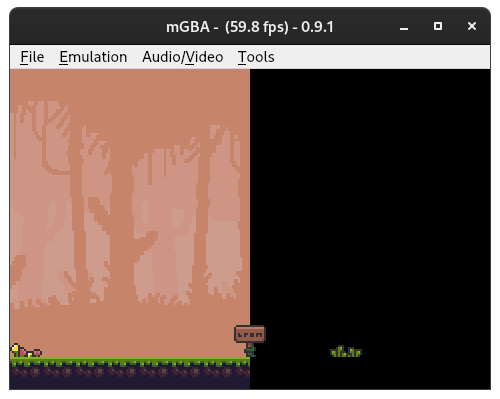
\includegraphics[width=.45\textwidth]{capitulos/capitulo3/window_1.png}
	\caption{Demostración del funcionamiento de una ventana.}
	\label{fig:windows}
\end{figure}


\chapter{Diseño y desarrollo del juego}\label{sec:desarrollo}

El objetivo principal del proyecto, desde el punto de vista técnico, es el desarrollo de un videojuego para la Game Boy Advance usando el menor número posible de librerías externas. Forzando así un mayor entendimiento de cómo funciona el dispositivo junto con la lógica requerida para poder hacer ciertas funciones aunque ya se proporcionen en la mayoría de librerías existentes para la consola.

Completadas las dos primeras tareas de la planificación, el estudio de la arquitectura y de técnicas de programación, se decide implantar una visión para el proyecto. Para ello, el autor revisita juegos de su agrado en los que basar el proyecto.

Una vez finalizado el proceso de búsqueda de inspiración, la idea inicial del proyecto fue la de recrear las mecánicas y jugabilidad del popular juego de PC \textit{Nidhogg} (véase la Figura~\ref{fig:nidhogg}).

\begin{figure}[h]
	\centering
	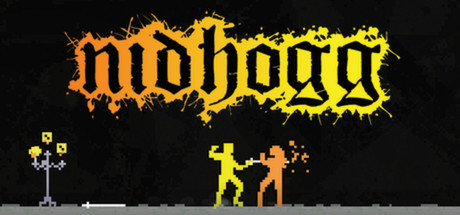
\includegraphics[width=.5\textwidth]{capitulos/capitulo5/nidhogg.jpg}
	\caption{Nidhogg, un juego para ordenador.}\label{fig:nidhogg}
\end{figure}
\FloatBarrier{}

El autor empezó a diseñar los \textit{assets} del juego recreándolos en \textit{Pixelorama}, tal y como se muestra en la Figura~\ref{fig:proto_1}.

\begin{figure}[h]
	\centering
	
\includegraphics[width=.6\textwidth]{capitulos/capitulo5/proto_1.png}
	\caption{\textit{Assets} para el primer prototipo del juego.}\label{fig:proto_1}
\end{figure}
\FloatBarrier{}

Sin embargo, al finalizar la primera iteración se observaron los siguientes riesgos que afectaban el desarrollo del juego:

\begin{itemize}
	\item Multijugador: Una de las fortalezas del juego original fue la posibilidad de conectar con otros jugadores y competir a través de la red, o en la propia máquina con múltiples mandos. Una implementación equivalente tendría que hacer uso de la comunicación serial que ofrece la consola, funcionalidad que dificulta probar el juego en hardware y que la mayoría de emuladores no soporta completamente, ya sea de forma local o en red. En la Figura~\ref{fig:mgba_serial_status} se muestra el estado actual de dicha funcionalidad en el emulador mGBA.

		\begin{figure}[h]
			\centering
			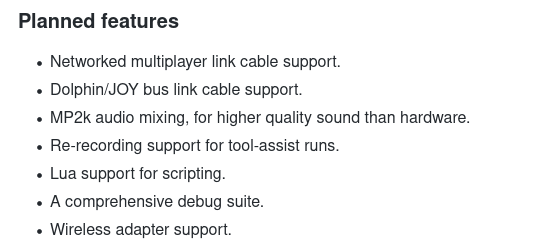
\includegraphics[width=.5\textwidth]{capitulos/capitulo5/mgba_serial_status.png}
			\caption{Funcionalidades por implementar.}\label{fig:mgba_serial_status}
		\end{figure}
		\FloatBarrier{}

	\item Arte: Otro error que se cometió en las primeras fases de desarrollo fue subestimar el tiempo requerido para crear los recursos o \textit{assets} del juego. Por este motivo, el autor decidió hacer uso de recursos \textit{open source} creados por la comunidad, utilizándolos siempre según las condiciones de las licencias utilizadas.
\end{itemize}

Habiendo reevaluado proyecto, se optó por realizar un juego de plataformas. El diseño giraría en torno a un personaje con diversas habilidades, siendo necesario familiarizarse con cada una de ellas para poder superar el juego.

En la segunda iteración se prototiparía un juego medieval (véase la Figura~\ref{fig:proto_2}) utilizando los \textit{assets} creados por \textit{Dagon}\footnote{https://im-dagon.itch.io/dungeon-pack} y acorde con las características descritas previamente. Sin embargo, antes de comenzar con el tercer sprint, se descartaría el diseño al no convencer al autor del proyecto.

\begin{figure}[h]
	\centering
	\includegraphics[width=.5\textwidth]{capitulos/capitulo5/proto_2.png}
	\caption{Segundo prototipo del juego.}\label{fig:proto_2}
\end{figure}
\FloatBarrier{}

Finalmente, a partir del tercer \textit{sprint} se optó por utilizar los \textit{assets} creados por \textit{o\_lobster}\footnote{https://o-lobster.itch.io/platformmetroidvania-pixel-art-asset-pack}. En la Figura~\ref{fig:proto_3} se ve una muestra del conjunto de recursos seleccionado en última instancia.

\begin{figure}[h]
	\centering
	\includegraphics[width=.5\textwidth]{capitulos/capitulo5/preview_lobster.png}
	\caption{Arte escogido para el desarrollo del juego.}\label{fig:proto_3}
\end{figure}
\FloatBarrier{}

A continuación, se detallarán los requisitos y las rutinas utilizadas para poder desarrollar el juego.

\section{Especificaciones}
En esta sección se describe la solución propuesta por el autor para satisfacer las necesidades del juego. La estructura de esta sección se deriva de asignaturas cursadas previamente~\cite{bib:diu}. Los acrónimos que se utilizarán en las próximas secciones son los siguientes:

\begin{itemize}
	\item \textbf{OBJ}: Objetivo (o requisitos generales del juego).
	\item \textbf{PU}: Perfil de Usuario.
	\item \textbf{ACT}: Actor del producto desarrollado.
	\item \textbf{RF}: Requisito Funcional.
	\item \textbf{RI}: Requisito de Información.
	\item \textbf{RNF}: Requisito No Funcional.
\end{itemize}

\subsection{Requisitos generales}
A continuación, se describen los requisitos generales del juego en forma de objetivos.

\begin{table}[h]
	\centering
	\begin{tabular}{| l | p{12cm} |}
		\hline
		\textbf{OBJ-1} & \textbf{Procesamiento de la entrada del jugador}  \\ \hline
		Versión & \gameversion{}  \\ \hline
		Descripción & El juego deberá procesar la entrada del usuario y actualizar los valores por pantalla, ya sea en los menús o en los niveles del juego.  \\ \hline
		Comentarios & Ninguno.  \\ \hline
	\end{tabular}
	\caption{Objetivo 1.}\label{tab:obj_1}
\end{table}

\begin{table}[h]
	\centering
	\begin{tabular}{| l | p{12cm} |}
		\hline
		\textbf{OBJ-2} & \textbf{Procesamiento de enemigos}  \\ \hline
		Versión & \gameversion{}  \\ \hline
		Descripción & El juego deberá actualizar de forma independiente la posición y estado de cualquiera de los enemigos que aparezcan en cada nivel del juego. \\ \hline
		Comentarios & Ninguno.  \\ \hline
	\end{tabular}
	\caption{Objetivo 2.}\label{tab:obj_2}
\end{table}

\begin{table}[h]
	\centering
	\begin{tabular}{| l | p{12cm} |}
		\hline
		\textbf{OBJ-3} & \textbf{Procesamiento de objetos}  \\ \hline
		Versión & \gameversion{}  \\ \hline
		Descripción & El juego deberá actualizar de forma independiente la posición y estado de cualquiera de los objetos que aparezcan en cada nivel del juego.  \\ \hline
		Comentarios & Ninguno.  \\ \hline
	\end{tabular}
	\caption{Objetivo 3.}\label{tab:obj_3}
\end{table}

\begin{table}[h]
	\centering
	\begin{tabular}{| l | p{12cm} |}
		\hline
		\textbf{OBJ-4} & \textbf{Procesamiento de las colisiones}  \\ \hline
		Versión & \gameversion{} \\ \hline
		Descripción & El juego deberá procesar las colisiones del jugador con objetos, enemigos y el entorno.  \\ \hline
		Comentarios & Ninguno.  \\ \hline
	\end{tabular}
	\caption{Objetivo 4.}\label{tab:obj_4}
\end{table}

\begin{table}[h]
	\centering
	\begin{tabular}{| l | p{12cm} |}
		\hline
		\textbf{OBJ-5} & \textbf{Gestión del progreso del jugador}  \\ \hline
		Versión & \gameversion{} \\ \hline
		Descripción & El juego deberá gestionar el progreso del jugador, de manera que el usuario no tenga que intervenir para tener una experiencia de juego continúa.  \\ \hline
		Comentarios & Ninguno. \\ \hline
	\end{tabular}
	\caption{Objetivo 5.}\label{tab:obj_5}
\end{table}
\FloatBarrier{}

\subsection{Casos de uso}
En esta sección se incluye el diagrama de casos de uso del juego y la especificación de los perfiles y actores que interactúan con el software. El diagrama se muestra en la Figura~\ref{fig:casos_uso}.

\begin{figure}[h]
	\centering
	\includegraphics[width=.7\textwidth]{capitulos/diagramas/casos_uso_2.png}
	\caption{Diagrama de casos de uso.}\label{fig:casos_uso}
\end{figure}
\FloatBarrier{}

Dado que el procesamiento del juego transcurre de forma local en la consola, mediante un dispositivo único, solo existe un actor en el sistema y por ende, un perfil de usuario. \\ \\

\begin{table}[h]
	\centering
	\begin{tabular}{| l | p{10cm} |}
		\hline
		\textbf{PU-1} & \textbf{Jugador}  \\ \hline
		Descripción & Perfil utilizado para identificar cualquier usuario que juegue al producto desarrollado, tanto en emuladores como en hardware.  \\ \hline
		Actores asociados & ACT-1 (Jugador) \\ \hline
		Comentarios & Ninguno.  \\ \hline
	\end{tabular}
	\caption{Perfil de Usuario 1.}\label{tab:pu-1}
\end{table}

\begin{table}[h]
	\centering
	\begin{tabular}{| l | p{10cm} |}
		\hline
		\textbf{ACT-1} & \textbf{Jugador}  \\ \hline
		Perfil de usuario & PU-1 \\ \hline
		Requisitos asociados & RF-1, RF-2, RF-3, RF-4, RF-5, RF-6, RF-7 \\ \hline
		Descripción & Formado por la persona que juega y utiliza el software desarrollado. \\ \hline
		Comentarios & Ninguno.  \\ \hline
	\end{tabular}
	\caption{Actor 1.}\label{tab:act-1}
\end{table}
\FloatBarrier{}

\subsection{Requisitos funcionales}
En esta sección se incluirán los requisitos funcionales del proyecto, extraídos del diagrama de casos de uso.

%\multicolumn{2}{c|}

\begin{table}[h]
	\centering
	\begin{tabular}{| l | p{11cm} |}
		\hline
		\textbf{RF-1} & \textbf{Jugar} \\ \hline
		Objetivos asociados & OBJ-1, OBJ-2, OBJ-3, OBJ-4 \\ \hline
		Requisitos asociados & RI-1 \\ \hline
		Descripción & El jugador inicia la partida. \\ \hline
		Precondición & El jugador debe haber encontrarse en el menú principal.  \\ \hline
		Secuencia normal & 
		\begin{enumerate}
			\item Mover el cursor al botón adecuado.
			\item El jugador presiona ``A''.
			\item Se carga el último nivel que no haya sido superado.
		\end{enumerate}
		\\ \hline
		Postcondición & El jugador inicia una partida. \\ \hline
		Excepciones & Ninguna. \\ \hline
		Comentarios & Ninguno. \\ \hline
	\end{tabular}
	\caption{Requisito funcional 1.}\label{tab:rf-1}
\end{table}

\begin{table}[h]
	\centering
	\begin{tabular}{| l | p{11cm} |}
		\hline
		\textbf{RF-2} & \textbf{Ver controles} \\ \hline
		Objetivos asociados & OBJ-1 \\ \hline
		Requisitos asociados & Ninguno. \\ \hline
		Descripción & El jugador selecciona la visualización de los controles. \\ \hline
		Precondición & El jugador debe haber encontrarse en el menú principal.  \\ \hline
		Secuencia normal & 
		\begin{enumerate}
			\item Mover el cursor al botón adecuado.
			\item El jugador presiona ``A''.
			\item El juego carga los nombres por pantalla.
		\end{enumerate}
		\\ \hline
		Postcondición & El jugador visualiza los controles por pantalla. \\ \hline
		Excepciones & Ninguna. \\ \hline
		Comentarios & Ninguno. \\ \hline
	\end{tabular}
	\caption{Requisito funcional 2.}\label{tab:rf-2}
\end{table}

\begin{table}[h]
	\centering
	\begin{tabular}{| l | p{11cm} |}
		\hline
		\textbf{RF-3} & \textbf{Acceder al menú in-game} \\ \hline
		Objetivos asociados & OBJ-1 \\ \hline
		Requisitos asociados & Ninguno. \\ \hline
		Descripción & El jugador accede al menú del juego. Desde ahí puede seleccionar varias opciones \\ \hline
		Precondición & El jugador debe encontrarse en mitad de una partida.  \\ \hline
		Secuencia normal & 
		\begin{enumerate}
			\item El jugador presiona ``Start''.
			\item El juego carga un menú sobre la partida actual.
		\end{enumerate}
		\\ \hline
		Postcondición & El jugador visualiza los un menú. \\ \hline
		Excepciones & Ninguna. \\ \hline
		Comentarios & Las físicas del juego se ven pausadas ya que la ``delta'' del juego no se actualiza. \\ \hline
	\end{tabular}
	\caption{Requisito funcional 3.}\label{tab:rf-3}
\end{table}

\begin{table}[h]
	\centering
	\begin{tabular}{| l | p{11cm} |}
		\hline
		\textbf{RF-4} & \textbf{Mover personaje} \\ \hline
		Objetivos asociados & OBJ-1, OBJ-4 \\ \hline
		Requisitos asociados & Ninguno. \\ \hline
		Descripción & El jugador mueve el personaje principal. \\ \hline
		Precondición & El jugador debe encontrarse en mitad de una partida.  \\ \hline
		Secuencia normal & 
		\begin{enumerate}
			\item El jugador presiona cualquiera de los que habilitan el movimiento del personaje.
			\item El juego actualiza la posición del personaje según la entrada del jugador.
			\item El juego comprueba cualquier tipo de colisión para actualizar el estado del jugador o sobrescribir la posición del mismo.
		\end{enumerate}
		\\ \hline
		Postcondición & El personaje ve actualizada su posición y estado. \\ \hline
		Excepciones & Ninguna. \\ \hline
		Comentarios & Ninguno. \\ \hline
	\end{tabular}
	\caption{Requisito funcional 4.}\label{tab:rf-4}
\end{table}

\begin{table}[h]
	\centering
	\begin{tabular}{| l | p{11cm} |}
		\hline
		\textbf{RF-5} & \textbf{Atacar} \\ \hline
		Objetivos asociados & OBJ-1, OBJ-4 \\ \hline
		Requisitos asociados & Ninguno. \\ \hline
		Descripción & El jugador ataca. \\ \hline
		Precondición & El jugador debe encontrarse en mitad de una partida y el personaje no puede estar en el aire.  \\ \hline
		Secuencia normal & 
		\begin{enumerate}
			\item El jugador presiona ``B''.
			\item El juego comprueba si existe contacto con algún enemigo.
			\item En caso afirmativo, el juego procesa el ataque.
		\end{enumerate}
		\\ \hline
		Postcondición & En caso de contacto, los enemigos ven actualizado su estado. \\ \hline
		Excepciones & Ninguna. \\ \hline
		Comentarios & Ninguno. \\ \hline
	\end{tabular}
	\caption{Requisito funcional 5.}\label{tab:rf-5}
\end{table}

\begin{table}[h]
	\centering
	\begin{tabular}{| l | p{11cm} |}
		\hline
		\textbf{RF-6} & \textbf{Reanudar partida} \\ \hline
		Objetivos asociados & OBJ-1 \\ \hline
		Requisitos asociados & Ninguno. \\ \hline
		Descripción & El jugador reanuda la partida después de haber pausado el juego. \\ \hline
		Precondición & El jugador debe encontrarse en el menú in-game.  \\ \hline
		Secuencia normal & 
		\begin{enumerate}
			\item Mover el cursor al botón adecuado.
			\item El jugador presiona ``A''.
			\item El juego desocupa los recursos que utilizaba el menú in-game y reanuda la partida.
		\end{enumerate}
		\\ \hline
		Postcondición & La partida es reanudada y la ``delta'' vuelve a actualizarse. \\ \hline
		Excepciones & Ninguna. \\ \hline
		Comentarios & Ninguno. \\ \hline
	\end{tabular}
	\caption{Requisito funcional 6.}\label{tab:rf-6}
\end{table}
\FloatBarrier{}

\begin{table}[h]
	\centering
	\begin{tabular}{| l | p{11cm} |}
		\hline
		\textbf{RF-7} & \textbf{Salir al menú principal} \\ \hline
		Objetivos asociados & OBJ-1 \\ \hline
		Requisitos asociados & Ninguno. \\ \hline
		Descripción & El jugador vuelve al menú principal del juego. \\ \hline
		Precondición & El jugador debe encontrarse en el menú in-game.  \\ \hline
		Secuencia normal & 
		\begin{enumerate}
			\item Mover el cursor al botón adecuado.
			\item El jugador presiona ``A''.
			\item El juego desocupa los recursos que utilizaba el nivel del juego y carga el menú principal.
		\end{enumerate}
		\\ \hline
		Postcondición & El juego carga el menú principal. \\ \hline
		Excepciones & Ninguna. \\ \hline
		Comentarios & Ninguno. \\ \hline
	\end{tabular}
	\caption{Requisito funcional 7.}\label{tab:rf-7}
\end{table}

\subsection{Requisitos de información}
En esta sección se incluirán los requisitos de información del proyecto. Esto solo involucra el progreso que ha hecho el jugador en previas sesiones de juego.

\vspace{2cm}

\begin{table}[h]
	\centering
	\begin{tabular}{| l | p{11cm} |}
		\hline
		\textbf{RI-1} & \textbf{``Save file''} \\ \hline
		Objetivos asociados & OBJ-5 \\ \hline
		Requisitos asociados & Ninguno. \\ \hline
		Descripción & El juego debe almacenar el progreso realizado por el jugador. \\ \hline
		Datos específicos & 
		\begin{itemize}
			\item Último nivel completado: Número entero.
		\end{itemize}
		\\ \hline
		Comentarios & Ninguno. \\ \hline
	\end{tabular}
	\caption{Requisito de información 1.}\label{tab:ri-1}
\end{table}
\FloatBarrier{}
\newpage
\subsection{Requisitos no funcionales}
En esta sección se incluirán los requisitos no funcionales del proyecto.

\vspace{2cm}

\begin{table}[h]
	\centering
	\begin{tabular}{| l | p{11cm} |}
		\hline
		\textbf{RNF-1} & \textbf{Rendimiento} \\ \hline
		Objetivos asociados & OBJ-1, OBJ-2, OBJ-3, OBJ-4 \\ \hline
		Requisitos asociados & Ninguno. \\ \hline
		Descripción & Con la finalidad de ofrecer una experiencia jugable agradable al jugador, el juego tiene como objetivo ofrecer una tasa de refresco de 60 fotogramas por segundo. Para ello se utiliza en la medida de lo posible cualquier opción que acelere el procesamiento del juego por medio de hardware. \\ \hline
		Comentarios & En el caso del proyecto, se ha optado por utilizar tiles y sprites antes que el modo bitmap. También se debe tener en cuenta las limitaciones y ventajas que ofrece el hardware del dispositivo, un ejemplo de ello es utilizar en la medida de lo posible enteros de 32 bits como tipo de datos o evitar hacer escrituras de 1 byte en la VRAM. \\ \hline
	\end{tabular}
	\caption{Requisito no funcional 1.}\label{tab:rnf-1}
\end{table}

\vspace{2cm}

\begin{table}[h]
	\centering
	\begin{tabular}{| l | p{11cm} |}
		\hline
		\textbf{RNF-2} & \textbf{Batería} \\ \hline
		Objetivos asociados & OBJ-1, OBJ-2, OBJ-3, OBJ-4 \\ \hline
		Requisitos asociados & Ninguno. \\ \hline
		Descripción & El juego además de tener que ofrecer un buen rendimiento, debe tener como prioridad maximizar el uso de la batería cuando sea posible. \\ \hline
		Comentarios & De manera simplificada, el objetivo es hacer que el procesador se encuentre el máximo tiempo posible en un estado de baja energía (mediante el uso de interrupciones por ejemplo). \\ \hline
	\end{tabular}
	\caption{Requisito no funcional 2.}\label{tab:rnf-2}
\end{table}

\begin{table}[h]
	\centering
	\begin{tabular}{| l | p{11cm} |}
		\hline
		\textbf{RNF-3} & \textbf{Accesibilidad y usabilidad} \\ \hline
		Objetivos asociados & OBJ-1 \\ \hline
		Requisitos asociados & Ninguno. \\ \hline
		Descripción & El producto desarrollado debe ofrecer una experiencia familiar y similar, en cuánto a controles se refiere, a otros juegos. Además, la estética y temática debe ser aceptable para cualquier tipo de público independientemente de la edad. \\ \hline
		Comentarios & Dado que el juego tiene que proporcionar una experiencia aceptable para cualquier tipo de público independientemente de la edad, se ha optado por ofrecer una experiencia similar a lo que describe la calificación PEGI 3\tablefootnote{https://pegi.info/what-do-the-labels-mean}. \\ \hline
	\end{tabular}
	\caption{Requisito no funcional 3.}\label{tab:rnf-3}
\end{table}

\begin{table}[h]
	\centering
	\begin{tabular}{| l | p{11cm} |}
		\hline
		\textbf{RNF-4} & \textbf{Mantenibilidad} \\ \hline
		Objetivos asociados & OBJ-1, OBJ-2, OBJ-3, OBJ-4, OBJ-5 \\ \hline
		Requisitos asociados & Ninguno. \\ \hline
		Descripción & Facilitar la comprensión, y posible contribución en un futuro, de personas ajenas al desarrollo inicial del juego. \\ \hline
		Comentarios & El desarrollo del código se llevará a cabo acorde con las pautas marcadas por el \textit{Linux kernel coding style} elaborado por el equipo de desarrollo del kernel Linux. \\ \hline
	\end{tabular}
	\caption{Requisito no funcional 4.}\label{tab:rnf-4}
\end{table}
\FloatBarrier{}

\begin{table}[h]
	\centering
	\begin{tabular}{| l | p{11cm} |}
		\hline
		\textbf{RNF-5} & \textbf{Administración del progreso del jugador} \\ \hline
		Objetivos asociados & OBJ-5 \\ \hline
		Requisitos asociados & RI-1 \\ \hline
		Descripción & Crear una experiencia de juego continua, sin cortes, donde el progreso del jugador se guardará sin que este tenga que manualmente especificarlo. \\ \hline
		Comentarios & El progreso del jugador solo se verá actualizado cuando este supere un nivel que no haya superado anteriormente. \\ \hline
	\end{tabular}
	\caption{Requisito no funcional 5.}\label{tab:rnf-5}
\end{table}

\section{Desarrollo}\label{sec:aspectos}
Una vez comentadas las especificaciones del proyecto, se dedica esta sección a comentar el funcionamiento específico de varias partes del código. Para una visión general del código se ha optado por utilizar diagramas de flujo, mientras que para una descripción específica del código se ha optado por utilizar pseudocódigo. Además, se comentarán aspectos destacables del desarrollo realizado. La estructura general se inspira en~\cite{bib:ing_vid}. 

\subsection{Menú}
El diagrama de flujo del menú se puede observar en la Figura~\ref{fig:flujo_menu}, siendo lo único destacable del proceso el procesamiento de la entrada del usuario.

Una vez transicionado del inicio a la escena donde se muestra el menú del juego, se cargan los \textit{assets} que se utilizarán para el menú principal y se lee cualquier dato guardado de partidas previas. Posteriormente, en un bucle infinito, se procede a actualizar las animaciones y posiciones de los \textit{sprites} y fondos del menú (el menú es dinámico). En cada iteración del bucle, se consulta el ``input'' del usuario y en caso de no reconocer el botón presionado como válido se vuelve al inicio del bucle, actualizando los elementos que no controla el jugador y esperando a que se acabe de renderizar el fotograma actual.

En caso de ser válido, se comprueba si el ``input'' mueve el cursor o presiona el botón seleccionado. En caso de mover el cursor, se actualiza la posición del \textit{sprite}. En caso de presionar el botón seleccionado, se cargará la siguiente escena. 

\begin{figure}[h]
	\centering
	\includegraphics[width=.5\textwidth]{capitulos/diagramas/flujo_menu.png}
	\caption{Diagrama de flujo del menú principal.}\label{fig:flujo_menu}
\end{figure}
\FloatBarrier{}

\subsection{Nivel del juego}
Para cada nivel del juego, se lee la entrada del usuario y se procesa de forma acorde, además de actualizar de forma independiente los enemigos y objetos del nivel. El proceso se puede observar en la Figura~\ref{fig:flujo_nivel}.

\begin{figure}[h]
	\centering
	\includegraphics[width=.65\textwidth]{capitulos/diagramas/flujo_nivel.png}
	\caption{Diagrama de flujo para cada nivel del juego.}\label{fig:flujo_nivel}
\end{figure}
\FloatBarrier{}

A diferencia del menú, el cual no contaba con enemigos, en el bloque de ``Actualizar animaciones y renderizado de sprites'' también se actualizan las posiciones de enemigos y objetos que puedan aparecer en el nivel. De forma adicional, se dedica un bloque al procesamiento de colisiones en los que se tiene en cuenta el entorno y otras entidades. Dado que para completar el nivel se tienen que cumplir ciertas condiciones, al final de cada iteración del bucle se comprueba si las condiciones se han cumplido y si el jugador debe reiniciar el nivel actual o pasar al siguiente. Es importante recalcar que el jugador no puede guardar manualmente el progreso, este solo se puede guardar en caso de que el jugador consiga pasar al siguiente nivel.

También, como se hizo referencia en el diagrama de casos de uso, se permite acceder a un menú in-game. El proceso es similar al visto en menú principal pero con ligeros cambios tal y como se puede observar en la Figura~\ref{fig:flujo_ingame}.


\begin{figure}[h]
	\centering
	\includegraphics[width=.5\textwidth]{capitulos/diagramas/flujo_ingame.png}
	\caption{Diagrama de flujo para el menú in-game.}\label{fig:flujo_ingame}
\end{figure}
\FloatBarrier{}

El bloque de ``Colisiones'', mostrado en la Figura~\ref{fig:flujo_nivel}, sigue los pasos mostrados a continuación para procesar las colisiones del juego:

\begin{itemize}
	\item Comprueba las colisiones del entorno en el eje X del personaje principal.
	\item Comprueba las colisiones del entorno en el eje Y del personaje principal.
	\item Comprueba las colisiones del entorno en el eje X de los enemigos.
	\item Comprueba las colisiones entre los enemigos y el personaje principal.
\end{itemize}

A continuación, se mostrará el pseudocódigo de cada uno de los apartados que conforma el bloque de ``Colisiones''. Las funciones mostradas (Algoritmos~\ref{algo:col_entorno_x} y~\ref{algo:col_entorno_y}) se han simplificado, omitiendo el procesamiento necesario al trabajar con valores desplazados por 8 bits (representación de coma fija).

Sin embargo, antes de mostrar el pseudocódigo destinado a las colisiones, se muestra el Listado~\ref{lst:se_index}, utilizada para conseguir el índice de un \textit{tile} específico. La función no sigue el cálculo habitual de $x+y*w$\footnote{Los fondos que utilizan la matriz de transformación si siguen la ecuación convencional, pero para el proyecto se utilizarán fondos ``normales'', en los cuales hay que seguir la metodología mostrada.} por culpa de la distribución no uniforme de los \textit{tiles} en la VRAM~\cite{bib:tonc}.

\vspace{1cm}

\begin{lstlisting}[language=c,label=lst:se_index,caption=Fragmento de código de la librería TONC.]
uint32_t se_index(uint32_t y, uint32_t x)
{
	// n = x + y * 32
	uint32_t n = x + (y << 5);

	if(x >= 32) {
		n += 0x03E0;
	}

	if(y >= 32 && IS_BG_512x512) {
		n += 0x0400;
	}

	return n;
}
\end{lstlisting}

\vspace{2cm}

\begin{algorithm}[h]
	\SetAlgorithmName{Algoritmo}{}
	\footnotesize
	\caption{Procesa el incremento en el eje X teniendo en cuenta el entorno.}
	\label{algo:col_entorno_x}
	\DontPrintSemicolon % Some LaTeX compilers require you to use \dontprintsemicolon instead
	\KwIn{y, x, incremento}
	\KwOut{incremento}

	\tcp{Si se mueve a la derecha, se añade un offset}
	\If{$incremento > 0$} {
		$x \gets x + offset$\;
	}

	\tcp{Cada tile ocupa 8 píxeles}
	$incTiles \gets abs(incremento) / 8$\;
	\tcp{Se recorre cada tile recorrido con el incremento}
	\For{$i \gets 0$ \textbf{to} $incTiles$} {
		\tcp{Se recorre el espacio que ocupa la altura del personaje}
		\For{$j \gets 0$ \textbf{to} $alturaPersonaje$} {
			\tcp{Se suma i en caso de ir a la derecha}
			\tcp{y se resta en caso de ir a la izquierda}
			$tile \gets getTileMapa(y+j, x{\pm}i)$\;
			\If{$tile\;es\;prohibido$} {
				$incremento \gets maxIncPermitido(x,i)$\;
				\Return{$incremento$}\;
			}
		}
		}
		\Return{$incremento$}\;
\end{algorithm}

\begin{algorithm}[h]
	\SetAlgorithmName{Algoritmo}{}
	\footnotesize
	\caption{Procesa el incremento en el eje Y teniendo en cuenta el entorno.}
	\label{algo:col_entorno_y}
	\DontPrintSemicolon % Some LaTeX compilers require you to use \dontprintsemicolon instead
	\KwIn{y, x, incremento}
	\KwOut{incremento}

	\tcp{Si se mueve hacia abajo, se añade un offset}
	\If{$incremento > 0$} {
		$y \gets y + offset$\;
	}

	\tcp{Cada tile ocupa 8 píxeles}
	$incTiles \gets abs(incremento) / 8$\;
	\tcp{Se recorre cada tile recorrido con el incremento}
	\For{$i \gets 0$ \textbf{to} $incTiles$} {
		\tcp{Se recorre el espacio que ocupa la anchura del personaje}
		\For{$j \gets 0$ \textbf{to} $anchuraPersonaje$} {
			\tcp{Se suma i en caso de ir abajo}
			\tcp{y se resta en caso de ir arriba}
			$tile \gets getTileMapa(y{\pm}i, x+j)$\;
			\If{$tile\;es\;prohibido$} {
				$incremento \gets maxIncPermitido(y,i)$\;
				\Return{$incremento$}\;
			}
		}
		}
		\Return{$incremento$}\;
\end{algorithm}
\FloatBarrier{}

En el caso de los enemigos, la dirección en la que se mueven se ve afectada por las colisiones que detecten. En caso de colisionar, el enemigo se invertirá y moverá en la dirección contraria. Por razones de optimización se omiten:

\begin{itemize}
	\item La comprobación del eje Y dado que los enemigos no pueden saltar. Para comprobar si los enemigos se acercan a una posición en caída libre, se comprobará el \textit{tile} posicionado debajo. De ahí el $alturaEnemigo+1$.
	\item El cálculo del mayor incremento permitido dado que no afectará de forma considerable la jugabilidad. Esta es la razón por la que se retorna 0 dentro del bucle.
\end{itemize}

A diferencia del movimiento del personaje, el movimiento de los enemigos se realiza de forma independiente. En cada iteración se llamará a un método que recorrerá todos los enemigos vivos para actualizar su posición utilizando el Algoritmo~\ref{algo:pos_enemigo}. Es necesario aclarar el uso del parámetro $a$, valor que será diferente dependiendo del enemigo. Si el movimiento del enemigo no permite el movimiento por ``aire'', el parámetro $a$ será mayor o igual a 1. En caso de que el movimiento del personaje permita desplazarse sin tener ningún bloque sólido debajo, el valor del parámetro $a$ será 0.

\begin{algorithm}[h]
	\SetAlgorithmName{Algoritmo}{}
	\footnotesize
	\caption{Procesa el incremento en el eje X del enemigo teniendo en cuenta el entorno.}
	\label{algo:pos_enemigo}
	\DontPrintSemicolon % Some LaTeX compilers require you to use \dontprintsemicolon instead
	\KwIn{y, x, incremento}
	\KwOut{incremento}

	\tcp{Si se mueve a la derecha, se añade un offset}
	\If{$incremento > 0$} {
		$x \gets x + offset$\;
	}

	\tcp{Cada tile ocupa 8 píxeles}
	$incTiles \gets abs(incremento) / 8$\;
	\tcp{Se recorre cada tile recorrido con el incremento}
	\For{$i \gets 0$ \textbf{to} $incTiles$} {
		\tcp{Se recorre el espacio que ocupa la altura del enemigo + a}
		\tcp{a denota si el enemigo procesará los bloques que estén debajo}
		\For{$j \gets 0$ \textbf{to} $alturaEnemigo+a$} {
			\tcp{Se suma i en caso de ir a la derecha}
			\tcp{y se resta en caso de ir a la izquierda}
			$tile \gets getTileMapa(y+j, x{\pm}i)$\;
			\If{$tile\;es\;prohibido$} {
				\Return{$0$}\;
			}
		}
		}
		\Return{$incremento$}\;
\end{algorithm}

Finalmente, la detección de colisiones entre el personaje principal y los enemigos se realiza tal y como se muestra en el Algoritmo~\ref{algo:collisions}.

\begin{algorithm}[h]
	\SetAlgorithmName{Algoritmo}{}
	\footnotesize
	\caption{Procesa las colisiones entre los enemigos y el personaje.}
	\label{algo:collisions}
	\DontPrintSemicolon % Some LaTeX compilers require you to use \dontprintsemicolon instead
	\KwIn{numeroEnemigos}

	\If{$personaje.estado\;esta\;siendo\;atacado$} {
		\Return{}\;
	}

	\tcp{Se recorren todos los enemigos vivos}
	\For{$i \gets 0$ \textbf{to} $numeroEnemigos$} {
		\tcp{Si la distancia entre las dos entidades es menor}
		\tcp{que la distancia minima declarada para el eje Y}
		\tcp{continuar comprobando el eje X}
		\If{$abs(personaje.y - enemigos[i].y) < distColisionY$} {
			\If{$abs(personaje.x - enemigos[i].x) < distColisionX$} {
				$personaje.estado \gets ATACADO$\;
				$personaje.vida \gets personaje.vida - 1$\;
			}
			$posicionEspada \gets personaje.x \pm offset$\;
			\If{$atacando \And abs(posicionEspada-enemigos[i].x) < distColisionX$} {
				$enemigos.vida \gets enemigos.vida - 1$\;
			}
		}
	}
\end{algorithm}
\FloatBarrier{}

\section{Aspectos destacados del desarrollo}
En esta sección, se comentan los aspectos a tener en cuenta del desarrollo y algunas de las prácticas y conocimientos obtenidos en la tarea de ``Estudio de las técnicas de programación'' programada en la planificación del proyecto.

\subsection{Pruebas de rendimiento}
La GBA no es un sistema convencional dado que no tiene una forma de mostrar información fácilmente por pantalla. Es por esto, que para las pruebas de rendimiento realizadas se ha utilizado un sistema peculiar. Entre las formas que se han utilizado para medir el rendimiento se distinguen:

\begin{itemize}
	\item Medida que incluye No\$GBA en su interfaz para comprobar rápidamente la carga de la CPU (véase la Figura~\ref{fig:nogba_bench}). A pesar de ser un medio poco fiable, es de utilidad para hacerse una idea general del rendimiento, y para distinguir de inmediato rutinas con una amplia diferencia de rendimiento.

		\begin{figure}[h]
			\centering
			\includegraphics[width=.5\textwidth]{capitulos/capitulo5/nogba_bench.png}
			\caption{Interfaz que utiliza No\$GBA para mostrar el uso de la CPU.}\label{fig:nogba_bench}
		\end{figure}
		\FloatBarrier{}

	\item Uso de los temporizadores que incluye la consola para medir con más precisión. La visualización de los valores puede consultarse en el depurador o por pantalla. Dado que las pruebas se realizan también en hardware, se ha optado por mostrar los valores por pantalla dado que no se cuenta con el hardware necesario para mantener una conexión JTAG (véase la Figura~\ref{fig:bench_value}).

		\begin{figure}[h]
			\centering
			\includegraphics[width=.6\textwidth]{capitulos/capitulo5/bench_value.png}
			\caption{El valor del temporizador en la esquina superior izquierda.}\label{fig:bench_value}
		\end{figure}
		\FloatBarrier{}

		Un ejemplo donde se comparó la eficiencia de dos fragmentos de código, fue en la carga de \textit{assets} antes de iniciar una escena en el juego. Para la prueba se comparó el tiempo que transcurría al copiar los datos utilizando \textit{DMA} y la función \textit{memcpy}. El código utilizado es similar al mostrado en el Listado~\ref{lst:benchmark}.

		\vspace{1cm}

	\begin{lstlisting}[language=c,caption={Tomando medidas mediante temporizadores.},label={lst:benchmark}]

	// Se activa el temporizador a f = 262.21 KHz
	*((volatile uint16_t*)0x04000102) = 0x0081;

	// Se copian los datos ...

	// Se consigue el valor del temporizador
	timer = *((volatile uint16_t*)0x04000100);

	// Se desactiva el temporizador
	*((volatile uint16_t*)0x04000102) = 0x0000;

	// Se muestra el valor por pantalla ...

	\end{lstlisting}

		Con los valores del \textit{benchmark} obtenidos, se divide la frecuencia utilizada entre el temporizador para hallar los segundos que han transcurrido. En el caso del ejemplo anterior los resultados se muestran en la Figura~\ref{fig:plot_bench}. Con estos resultados se llegó a la conclusión de cargar los datos mediante \textit{DMA} era la opción más adecuada. 

		\begin{figure}[h]
			\centering
			\includegraphics[width=.55\textwidth]{capitulos/capitulo5/graph_bench.png}
			\caption{Resultados de la prueba de rendimiento.}\label{fig:plot_bench}
		\end{figure}
\end{itemize}
\FloatBarrier{}

\subsection{Sincronización vertical}
Uno de los primeros problemas que surgieron en el desarrollo del juego, fue la desincronización vertical que se producía al actualizar los fondos y~\textit{sprites} por pantalla. Este fenómeno se produce cuando se actualizan objetos mientras la pantalla se está actualizando. Una instancia donde se puede observar este problema se muestra en la Figura~\ref{fig:torn}, en concreto en la parte superior de la imagen. Aquí, se puede observar la distorsión que se produce en el personaje y la moneda. 

\begin{figure}[h]
	\centering
	\includegraphics[width=.4\textwidth]{capitulos/capitulo5/torn.png}
	\caption[Desincronización vertical.]{Desincronización vertical. Imagen obtenida de \cite{bib:washington}.}\label{fig:torn}
\end{figure}
\FloatBarrier{}

Inicialmente para resolver el problema, el programa se esperaba a que la consola terminase de renderizar el fotograma actual para cambiar las posiciones de los fondos y objetos. Para ello se comprueba el valor de VCount en la dirección de memoria 0x04000006 mediante dos bucles \textit{while} mostrados en el Listado~\ref{lst:vsync_1}~\cite{bib:tonc}. La finalidad del primer bucle es la de evitar actualizar el fotograma más de una vez cuando el procesamiento realizado se completa antes de renderizarse el siguiente fotograma.

\begin{lstlisting}[language=c,caption={Implementación de VSync mediante dos bucles.},label={lst:vsync_1}]
volatile uint16_t *vcount = (volatile uint16_t*)0x04000006;

while (*vcount >= 160);
while (*vcount < 160);

// Actualizar posiciones y estados ...
\end{lstlisting}

Sin embargo, esta implementación no es eficiente y no cumple con los requisitos no funcionales RNF-1 y RNF-2, dado que el procesador se encuentra al 100\% mientras espera para procesar el siguiente fotograma. La solución por lo tanto, es utilizar las interrupciones del sistema, evitando así un consumo excesivo del procesador y de la batería. Esto se consigue, con la instrucción de ensamblador \textit{swi}, la cual en la Game Boy Advance llamará a una de las funciones predefinidas de la BIOS. En este caso, la función que interesa utilizar es la 0x05, la función que pone al dispositivo en un estado de baja energía hasta que se produzca una interrupción VBlank. Para más información sobre las funciones disponibles consultar el Apéndice~\ref{ap:bios}.

Al abrir uno de los prototipos en el emulador No\$GBA, el cual ofrece una gráfica mostrando el uso del procesador, se puede observar una importante diferencia en consumo. En la Figura~\ref{fig:vsync_irq} se observa a la izquierda, el procesador al 100\% sin que ninguno de los personajes se mueva, mientras que a la derecha se observa un uso de la CPU casi inexistente al utilizar interrupciones.

\begin{figure}[h]
	\centering
	\begin{subfigure}[b]{0.45\textwidth}
		\centering
		\includegraphics[width=\textwidth]{capitulos/capitulo5/wout_irq.png}
		\label{fig:wout_irq}
		\caption{Rendimiento sin utilizar interrupciones.}
	\end{subfigure}
	\hfill
	\begin{subfigure}[b]{0.45\textwidth}
		\centering
		\includegraphics[width=\textwidth]{capitulos/capitulo5/with_irq.png}
		\label{fig:with_irq}
		\caption{Rendimiento utilizando interrupciones.}
	\end{subfigure}
	\caption{Rendimiento de las dos alternativas disponibles.}
	\label{fig:vsync_irq}
\end{figure}

\subsection{Operaciones de punto flotante}
Una limitación importante que se tuvo en cuenta en el desarrollo fue el rendimiento de la consola al operar números de coma flotante, y dividir y realizar operaciones de módulo. Esto se debe a la falta de una \textit{FPU} (Unidad de Punto Flotante) y una implementación por hardware de la división en la consola \cite{bib:tonc}. Para remediar estas limitaciones, se procura desplazar bits antes que realizar una división y utilizar números de coma fija. Es necesario mencionar que los compiladores optimizan automáticamente las divisiones en base 2, pero por razones de consistencia, en el código se utilizarán operaciones \textit{shift} incluso para las divisiones en base 2.

Una demostración de una operación con números representados con coma fija para la sentencia $\frac{1}{2}+\frac{1}{2}$, se observa en el Listado~\ref{lst:fixed_numbers}.

\begin{lstlisting}[language=c,caption={Ejemplo de un cálculo con números de coma fija.},label={lst:fixed_numbers}]
int a, b, c;
a = b = 1 << 8;

a = a >> 1;
b = b >> 1;

c = a + b;
c = c >> 8; // c = 1

\end{lstlisting}

A pesar de tener que realizar un preprocesamiento y postprocesamiento de los datos, sigue siendo más eficiente que realizar una división de coma flotante en un dispositivo sin \textit{FPU}.

\subsection{Limitaciones de lectura y escritura}
Otra limitación del hardware afecta las operaciones de escritura y lectura sobre ciertas direcciones de memoria. La más llamativa es la limitación de escritura de la VRAM, RAM de paleta y OAM. En estas tres secciones el programador no puede realizar escrituras de 1 byte. En el caso de tener que escribir 1 byte, se tiene que leer 2 bytes, sobrescribir el byte que se desea modificar y actualizar el valor.

Otro ejemplo, esta vez de lectura, se encuentra en la mayoría de registros I/O. Los espacios de memoria dedicados a modificar los \textit{offsets} de los fondos, se puede escribir pero no se puede leer los valores almacenados. Esta es la razón por la que se tienen que utilizar variables auxiliares al trabajar con ciertos registros de entrada y salida.

\subsection{Texto}
Las dos opciones que se barajaron para mostrar texto por pantalla en el juego fueron una implementación por \textit{sprites} y una implementación por mapa. La primera consiste en reservar un espacio de la OAM y representar cada letra mediante un \textit{sprite} diferente. La segunda implementación, consiste en incluir el texto en los fondos, incluyendo cada una de las letras en los \textit{tiles}.

La implementación por la optó el autor fue una híbrida. Para los créditos iniciales, menú principal, menú de controles y menú in-game se utilizó una implementación mediante \textit{sprites}. Esto permitía al programador modificar fácilmente el texto mostrado por pantalla. Por otro lado, para los niveles, en concreto las indicaciones mostradas en los niveles, se utilizó una implementación por mapa. De esta forma el programador no se tenía que preocupar de cambiar la posición del texto cuando el jugador se moviese por el nivel.

\subsection{Preparación de los archivos binarios}
Dada la gran cantidad de imágenes y archivos de audio utilizados, el autor utilizó Grit, SuperFamiconv y Audacity para convertir los archivos originales a un array de bytes con el que el programa pueda trabajar. Para las imágenes, se programó un \textit{script} de BASH que automatizase el proceso, creando un mapa para cada escena, un conjunto de \textit{tiles} para cada grupo de escenas y una paleta de colores a compartir entre todos los fondos. Un ejemplo de la salida generada se puede observar en la Figura~\ref{fig:script}. Los comandos ejecutados en el \textit{script} se pueden consultar en el Apéndice~\ref{ap:scripts}.

\begin{figure}[h]
	\centering
	\includegraphics[width=.8\textwidth]{capitulos/capitulo5/salida_script.png}
	\caption{Archivos generados por el \textit{script}.}\label{fig:script}
\end{figure}
\FloatBarrier{}

En el caso de los archivos de audio, se utilizó Audacity para convertir todas las pistas de audio a un solo canal y a una frecuencia de 16 KHz. El resultado se exportaría después a un formato ``raw'' sin ningún tipo de cabecera~\cite{bib:washington}.

Con los archivos ``.bin'' generados, el siguiente paso es utilizarlos en el código, para ello el Makefile utilizado (y proporcionado por el \textit{toolchain}) para el proyecto incluye una regla para enlazar todos los archivos binarios al proyecto (véase la Figura~\ref{fig:makefile}). Esta regla permitirá al programador referenciar los archivos incluyendo en la cabecera un archivo con el siguiente formato: ``archivo\_bin.h'' siendo archivo el nombre del archivo utilizado sin contar la extensión. La variable que guarda el valor del archivo y la variable que guarda el tamaño en bytes sigue un formato similar al de la cabecera: ``archivo\_bin'' y ``archivo\_bin\_size'' respectivamente.

\begin{figure}[h]
	\centering
	\includegraphics[width=.7\textwidth]{capitulos/capitulo5/makefile.png}
	\caption{Regla del Makefile.}\label{fig:makefile}
\end{figure}
\FloatBarrier{}

\chapter{Resultado final}\label{sec:final}
En esta sección se muestra el producto desarrollado, explicando en que consiste el juego y las decisiones con respecto al diseño que se han tomado. Todo el código del proyecto se puede encontrar en~\cite{bib:repositorio}, repositorio alojado en GitHub. La estructura del proyecto se puede consultar en el Apéndice~\ref{ap:estructura}. Además, en el repositorio se proporciona una versión del juego ya preparada para su prueba en emuladores o en hardware. Este archivo, junto al código de esa versión, se puede encontrar en la sección de ``Releases'' del repositorio. Un ejemplo de una versión publicada del juego se puede observar en la Figura~\ref{fig:release}.

\begin{figure}[h]
	\centering
	\includegraphics[width=.8\textwidth]{capitulos/capitulo6/release.png}
	\caption{Versión publicada del juego.}\label{fig:release}
\end{figure}
\FloatBarrier{}

\section{\textit{YAP} - \textit{Yet Another Platformer}}

\begin{figure}[b]
	\centering
	\includegraphics[width=.5\textwidth]{capitulos/capitulo6/logo.png}
	\caption{Logo del juego \textit{Yet Another Platformer}.}\label{fig:logo}
\end{figure}

El juego, titulado \textit{YAP} (\textit{Yet Another Platformer}, logo en la Figura~\ref{fig:logo}), pone al jugador en el lugar de un mago que tiene que progresar por cada nivel, derrotando a los enemigos que encuentre por el camino. Los controles utilizados para moverse por el mapa son los habituales para juegos de este género, el botón izquierdo para moverse a la izquierda y el botón derecho para moverse a la derecha.

El mago que controla el jugador deberá alternar entre dos formas distintas, la azul y dorada, para poder progresar en el juego. Esto se debe a que cada una de las variantes tiene habilidades imprescindibles para completar cada uno de los niveles:

\begin{itemize}
	\item Variante azul: La variante azul, la cual se activa pulsando el botón ``L'', permite al jugador moverse con más rapidez con tal de poder escapar con facilidad de los enemigos. Además permite al jugador saltar a las estructuras elevadas que encontrará en cada uno de los niveles presionando el botón ``A''. La limitación de esta variante aparece al enfrentarse con los enemigos ya que no puede atacar, para ello el jugador tendrá que transformarse en la variante dorada del mago.
	\item Variante dorada: La variante dorada, la cual se activa pulsando el botón ``R'', limita el movimiento del jugador, ralentizando su velocidad en el eje X e imposibilitando su movimiento en el eje Y. Sin embargo, ahora el jugador tiene la posibilidad de atacar a los enemigos que se encuentren en proximidad presionando el botón ``B''.
\end{itemize}

\section{Personajes}

Los personajes del juego, excepto por algunas modificaciones menores, son todos obra de \textit{\href{https://o-lobster.itch.io/}{o\_lobster}}. La primera versión del juego cuenta con el mago mostrado en el \textit{spritesheet} de la Figura~\ref{fig:hero}. En la primera fila se observan las imágenes utilizadas para cuando el personaje no se mueve. La segunda fila muestra las imágenes utilizadas para cuando el personaje se mueve por tierra. En la tercera y cuarta fila se observan las imágenes para cuando el personaje cae de una posición elevada y salta. En la quinta y sexta fila se observan las imágenes utilizadas para animar el ataque del personaje, siendo la quinta fila la correspondiente al personaje y la sexta la correspondiente a la espada que saca el mismo. Por último, la última fila, muestra las imágenes utilizadas para la animación de la muerte del personaje. Para separar la animación de muerte de las demás, se ha optado también por parar de actualizar todas las demás animaciones cuando se de el caso (dejando al personaje como la única entidad animada). Cada una de los estados que puede tener el personaje (inactivo, corriendo, saltando y atacando), se actualiza la animación cada 10 fotogramas. Este comportamiento también se observa para los enemigos. En caso de agotar las imágenes destinadas a un estado en particular, se vuelve a empezar por la primera imagen. Un estado que no se incluye en el \textit{spritesheet} es el estado cuando el personaje es atacado. Tomando como inspiración algunos juegos de la época, se ha optado por hacer que el \textit{sprite} parpadeé para señalar que ha recibido daño de un enemigo para así rebajar el número de \textit{tiles} utilizados. Este efecto se consigue activando y desactivando el \textit{sprite} cada cierto periodo de tiempo.

\begin{figure}[h]
	\centering
	\includegraphics[height=5cm]{capitulos/capitulo6/hero.png}
	\caption{Los \textit{sprites} del personaje principal.}\label{fig:hero}
\end{figure}
\FloatBarrier{}

La variante dorada del personaje utiliza exactamente el mismo \textit{spritesheet} de la Figura~\ref{fig:hero} pero especificando una paleta de colores alterna. La transición entre cada uno de los estados hace uso del efecto mosaico para así dar la sensación que el mago se está transformando. La Figura~\ref{fig:hero_variants} muestra a los dos personajes.


\begin{figure}[h]
	\centering
	\begin{subfigure}[b]{0.45\textwidth}
		\centering
		\includegraphics[width=\textwidth]{capitulos/capitulo6/hero_blue.png}
		\label{fig:hero_blue}
		\caption{Variante azul saltando.}
	\end{subfigure}
	\hfill
	\begin{subfigure}[b]{0.45\textwidth}
		\centering
		\includegraphics[width=\textwidth]{capitulos/capitulo6/hero_gold.png}
		\label{fig:hero_gold}
		\caption{Variante dorada atacando.}
	\end{subfigure}
	\caption{Las dos variantes del personaje principal.}
	\label{fig:hero_variants}
\end{figure}
\FloatBarrier{}

Los dos enemigos incluidos en el juego cuentan con animaciones y estados más simples que el personaje principal. El primer enemigo, el ``monstruo verde'' cuenta con dos estados, el estado en movimiento o inactivo, y el estado de muerte del enemigo. El \textit{spritesheet} se puede observar en la Figura~\ref{fig:slime}. Este enemigo se mueve de forma independiente hasta detectar una colisión en el eje X o vacío en el eje Y (una caída). Cuando detecta la colisión invertirá su posición.

\begin{figure}[h]
	\centering
	\includegraphics[height=2cm]{capitulos/capitulo6/slime.png}
	\caption{Los \textit{sprites} del primer enemigo.}\label{fig:slime}
\end{figure}

El otro enemigo, la ``mosca'', al igual que el ``monstruo verde'', cuenta con dos estados, el estado en movimiento o inactivo, y el estado de muerte del mismo. El \textit{spritesheet} se puede observar en la Figura~\ref{fig:fly}. A diferencia del ``monstruo verde'', este enemigo puede moverse sin tener ningún bloque sólido por debajo, aunque si se encuentra de frente con un bloque invertirá su orientación.

\begin{figure}[h]
	\centering
	\includegraphics[height=2cm]{capitulos/capitulo6/fly.png}
	\caption{Los \textit{sprites} del segundo enemigo.}\label{fig:fly}
\end{figure}

Los dos enemigos renderizados en un nivel se pueden observar en la Figura~\ref{fig:enemies}. Para una demostración más extensiva de los diferentes estados de cada personaje consultar el Apéndice~\ref{ap:personajes}.

\begin{figure}[h]
	\centering
	\includegraphics[width=.7\textwidth]{capitulos/capitulo6/enemies.png}
	\caption{Enemigos de uno de los niveles.}\label{fig:enemies}
\end{figure}

\section{\textit{Title screens}, menús y niveles}
Cada uno de los créditos, menús y niveles reciben el nombre de ``escenas'' en el código, término que se utiliza en motores gráficos como Unity. Los créditos iniciales del juego muestran el logo de la Universidad de Almería (aprovechando los fondos \textit{bitmap} del dispositivo) y todas las personas cuyos recursos han sido utilizados. Dos ejemplos, incluyendo el logo y el nombre del autor se pueden observar en la Figura~\ref{fig:credits}. Para el resto de escenas consultar el Apéndice~\ref{ap:escenas}.

La siguiente escena con la que el jugador se encuentra, una vez acabados los créditos iniciales del juego, es el menú principal. El menú principal cuenta con fondos y \textit{sprites} animados y una imagen proveniente del emulador se puede observar en la Figura~\ref{fig:menu}. Las diferencias observadas entre el menú actual y los mostrados previamente se deben a cambios durante el desarrollo del juego. El menú definitivo es el mostrado en la Figura~\ref{fig:menu}.

\begin{figure}[h]
	\centering
	\begin{subfigure}[b]{0.45\textwidth}
		\centering
		\includegraphics[width=\textwidth]{capitulos/capitulo5/game_0.png}
		\label{fig:credit_logo}
		\caption{\textit{Title screen} con el logo de la UAL.}
	\end{subfigure}
	\hfill
	\begin{subfigure}[b]{0.45\textwidth}
		\centering
		\includegraphics[width=\textwidth]{capitulos/capitulo5/game_1.png}
		\label{fig:credit_nombre}
		\caption{Game Boy Advance Micro}
	\end{subfigure}
	\caption{\textit{Title screen}.}
	\label{fig:credits}
\end{figure}
\FloatBarrier{}

\begin{figure}[h]
	\centering
	\includegraphics[width=.6\textwidth]{capitulos/capitulo6/menu.png}
	\caption{Menú principal del juego.}\label{fig:menu}
\end{figure}
\FloatBarrier{}

Aquí el jugador puede empezar una partida, o seguir el progreso en caso de haber jugador anteriormente, y consultar los controles del juego. En la escena de controles, se incluye un espacio para que el jugador pueda probarlos tal y como se puede observar en la Figura~\ref{fig:controls}.

\begin{figure}[h]
	\centering
	\includegraphics[width=.6\textwidth]{capitulos/capitulo6/controls.png}
	\caption{Escena de controles del juego.}\label{fig:controls}
\end{figure}
\FloatBarrier{}

El primer nivel del juego cuenta con pequeñas indicaciones para guiar al jugador durante su primera partida. Las dos escenas que conforman el primer nivel se pueden apreciar en la Figuras~\ref{fig:lvl1_0} y~\ref{fig:lvl1_1}. A pesar de no forzar al jugador a realizar las indicaciones mostradas, el diseño del primer nivel requiere que el jugador sepa realizar todas las acciones y funcionalidades para poder completarlo. El resto de niveles se puede observar en el Apéndice~\ref{ap:escenas}.

\vspace{1cm}

\begin{figure}[h]
	\centering
	\includegraphics[width=.55\textwidth]{capitulos/capitulo6/level_1_0.png}
	\caption{Primera parte del nivel.}\label{fig:lvl1_0}
\end{figure}

\begin{figure}[h]
	\centering
	\includegraphics[width=.9\textwidth]{capitulos/capitulo6/level_1_1.png}
	\caption{Segunda parte del nivel.}\label{fig:lvl1_1}
\end{figure}
\FloatBarrier{}

Todos los niveles del juego utilizan los 4 fondos ``normales'' que ofrece la GBA. El primero de ellos se reserva para cualquier estructura que provoque una colisión con el personaje y enemigos, el suelo por ejemplo. El segundo fondo se utiliza para aquellos objetos que forman parte del nivel pero no provocan colisiones. El tercer fondo, se reserva para el fondo naranja utilizado en la Figura~\ref{fig:menu}. Finalmente, el cuarto fondo se utiliza para guardar el menú in-game, el cual solo se activa si el jugador presionar ``Start''. 

\section{Música}
Dado que no se puede demostrar las dos piezas de música utilizadas para el juego, realizadas por \textit{\href{https://gooseninja.itch.io/}{Goose Ninja}}, se comentará brevemente la implementación por \textit{Direct Sound}.

En el juego, se hacen uso de dos muestras de audio, diseñadas para poder reproducirse en ciclo sin cortes. Para hacer posible su reproducción en el dispositivo, se han convertido a una frecuencia de 16 KHz a 8 bits. Cada ciclo se realiza a partir de los contadores del dispositivo y de las transferencias \textit{DMA} de tipo 1. Las transferencias además se configuran para que ocurran cada vez que el buffer de audio se quede vacío.

\section{Indicadores in-game}
El único indicador utilizado es el número de corazones (vida) con el que cuenta el personaje. El indicador se localiza en la esquina superior izquierda, y al aparecer el personaje realiza una pequeña animación para llamar la atención del jugador. A diferencia del resto animaciones, esta depende de la matriz de transformación ya que cambia la escala de un tamaño inapreciable al tamaño original en un corto periodo de tiempo. En la Figura~\ref{fig:heart} se pueden observar el estado inicial y final de la animación. Dado que los corazones denotan la vida del jugador, estos irán desapareciendo conforme el jugador pierde vida.

\begin{figure}[h]
	\centering
	\begin{subfigure}[b]{0.45\textwidth}
		\centering
		\includegraphics[width=\textwidth]{capitulos/capitulo6/heart_small.png}
		\label{fig:heart_small}
		\caption{Inicio de la animación.}
	\end{subfigure}
	\hfill
	\begin{subfigure}[b]{0.45\textwidth}
		\centering
		\includegraphics[width=\textwidth]{capitulos/capitulo6/heart_big.png}
		\label{fig:heart_big}
		\caption{Fin de la animación.}
	\end{subfigure}
	\caption{Tres corazones indicando la vida del jugador.}
	\label{fig:heart}
\end{figure}
\FloatBarrier{}


\section{Evaluación del juego en el hardware original}
En esta sección se mostrará el procedimiento a seguir para poder probar el juego en el hardware original. Para ello se hará uso de la tarjeta \textit{Supercard} adquirida junto con el software necesario para cargar el juego en la tarjeta. En el repositorio se incluirá una copia del software dado que no se puede asegurar su disponibilidad en los servidores utilizados por el fabricante para alojarlo.

Con el código compilado, ejecutando el comando ``make'' sobre el directorio raíz del proyecto, se ejecuta el programa ``Super Card'' (véase la Figura~\ref{fig:supercard_software}). Una vez abierto, en la ventana de opciones se seleccionará la tarjeta microSD que se introducirá en el cartucho. Seguidamente, en la ventana principal se seleccionará el juego para procesarlo y guardarlo en la tarjeta.

Seguidamente, se desconecta la tarjeta microSD y se introduce en el cartucho ``Supercard''. Al iniciar la consola, se mostrará un menú con la lista de todos los juegos instalados en la tarjeta. Para abrir el juego, basta con seleccionarlo con el pad direccional y el botón ``A''. En la Figura~\ref{fig:running} se puede observar  el juego ejecutándose en hardware de forma nativa.

\begin{figure}[h]
	\centering
	\includegraphics[width=.6\textwidth]{capitulos/capitulo6/supercard.png}
	\caption{Software para meter juegos en el cartucho.}\label{fig:supercard_software}
\end{figure}
\FloatBarrier{}

\begin{figure}[h]
	\centering
	\includegraphics[width=.8\textwidth]{capitulos/capitulo6/running.jpeg}
	\caption{El juego se ejecuta en la Nintendo DS.}\label{fig:running}
\end{figure}
\FloatBarrier{}

\chapter{Conclusiones del proyecto}\label{sec:conclusion}
En esta sección se realizará un balance del trabajo realizado indicando a su vez varias mejoras que pueden realizarse en las próximas versiones del producto.

El autor considera el proyecto uno de los más interesantes que ha realizado en la carrera, permitiéndole aplicar varios de los conocimientos adquiridos durante la misma. Los conocimientos aplicados varían enormemente, cubriendo conceptos como \textit{DMA} proporcionados en la asignatura de ``Periféricos e Interfaces'', el uso de ondas visto en la asignatura de ``Transmisión de Datos y Redes de Computadores'' e incluso algunos conceptos matemáticos en el área de matrices. El desarrollo de un juego para la Game Boy Advance también ha permitido un mejor entendimiento de varios de los dispositivos con los que el autor ha trabajado anteriormente, en concreto los microcontroladores Arduino y ESPRESSIF mencionados en la introducción del trabajo. Esto último demuestra la efectividad que tiene el dispositivo en el espacio educativo, tal y como se demostró en~\cite{bib:paper3,bib:paper_1,bib:paper_2}.

Además, el autor considera que actualmente tiene un mejor entendimiento de las tareas a realizar para proyectos futuros que involucren el desarrollo de un videojuego, identificando mejor las tareas que puede realizar y las que no. De las tareas que no se han podido realizar, como el diseño del arte y de la música, el autor considera que con más tiempo este aspecto podría haber sido mejorado dado que acabo siendo un factor limitante durante el desarrollo del juego. Otro aspecto a mejorar, relacionado con el arte del juego, es la poca cantidad de contenido disponible en el producto final ya que los enemigos, personajes y fondos dependían del contenido ``open source'' disponible online. 

A pesar de que el proyecto no ha quedado con los estándares que el autor deseaba, tiene la motivación no solo para seguir desarrollando el proyecto hasta conseguir una versión con la que esté satisfecho, sino para continuar desarrollando juegos para la Game Boy Advance. En sus próximos proyectos, espera combinar los conocimientos ya adquiridos con otros con finalidades más específicas como la comunicación serial que ofrece la consola para comunicarse con otros jugadores.

\section{Trabajo futuro}
A continuación se incluirán las mejoras que el autor considera implementar durante los próximos meses para alcanzar el nivel de calidad deseado. Las mejoras no incluyen las ``remodelaciones'' desde cero que desearía realizar el autor, sino mejoras inmediatas al producto actual.

\begin{itemize}
	\item Mejora del movimiento del jugador, haciendo que los controles sean más fluidos para el jugador.
	\item Mejora en las colisiones del jugador con el mapa. Actualmente las colisiones del jugador con el entorno se realizan de forma aproximada cuando este se mueve a una velocidad no exacta (por ejemplo, al moverse a $1.25$ píxeles por unidad de tiempo). 
	\item Buscar una implementación de la sincronización vertical que permita jugar al juego a 120 Hz en emuladores. El autor no ha investigado al respecto pero cree que es posible y una opción interesante dado que una gran parte de los jugadores utiliza emuladores en dispositivos considerablemente más potentes que la consola original. 
	\item Uso de efectos de sonido para las acciones del personaje principal (por ejemplo, al saltar y atacar). Estos se realizarían con los canales de audio 1, 2, 3 y 4.
	\item Implementación de un sistema de texto que permita el uso de más de un lenguaje. Actualmente el juego solo se encuentra en inglés.
	\item Implementación de un sistema que permita el uso de más de un mago. Esto permitiría añadir más variantes al juego (actualmente solo hay 2). El prototipo que el autor tenía en mente, sería uno similar al ofrecido por otros juegos con varias opciones a seleccionar. El jugador presionaría el botón ``L'' o ``R'', acción que abriría un menú, y con el pad direccional seleccionaría la variante a utilizar. Una imagen mostrando el prototipo se puede observar en la Figura~\ref{fig:menu_proto}.

	\begin{figure}[h]
		\centering
		\includegraphics[width=.5\textwidth]{capitulos/capitulo7/proto.png}
		\caption{Prototipo del nuevo sistema de selección.}\label{fig:menu_proto}
	\end{figure}
	\FloatBarrier{}

	\item Implementación de las secciones más costosas en ensamblador. El autor tiene pensado implementar las funciones encargadas de gestionar las colisiones de los enemigos y personaje principal.
\end{itemize}


\addcontentsline{toc}{chapter}{Bibliografía}
\bibliography{referencias}

%\appendix
%\clearpage
\begin{appendices}
%\addtocontents{toc}{ \vspace{5mm} \hrule \par}

\chapter{Contenido adicional}\label{sec:apendice}

\section{Estructura del proyecto}\label{ap:estructura}
La estructura escogida para el proyecto ha sido la marcada por el ``Makefile'' proporcionado por el \textit{toolchain} utilizado. La estructura es la observada en la Figura~\ref{fig:ap_estructura}.

\begin{figure}[h]
	\centering
	\includegraphics[width=.7\textwidth]{capitulos/apendice/estructura.png}
	\caption{Estructura del proyecto.}\label{fig:ap_estructura}
\end{figure}
\FloatBarrier{}

Cada uno de los archivos y directorios mostrados tiene la siguiente función:

\begin{itemize}
	\item data: En esta carpeta se localizan todos los archivos binarios, como imágenes y pistas de audio, que posteriormente son convertidas a un formato compatible con la consola.
	\item docs: Aquí reside el documento \LaTeX~junto con otros apuntes en sucio realizados durante el desarrollo del juego.
	\item include: Todas las cabeceras del código residen aquí.
	\item LICENSE: En este archivo se describen las condiciones de la licencia escogida, la MIT\footnote{https://opensource.org/licenses/MIT}.
	\item Makefile: El archivo que permite a ``make'' compilar el código y convertir los \textit{assets} del juego. Precisa una instalación previa de \textit{devkitpro} dado que utiliza varias herramientas incluidas en el \textit{toolchain}.
	\item README.md: En este archivo se incluyen varias instrucciones a los usuarios que visitan el repositorio GitHub.
	\item resources: En esta carpeta se incluyen varios recursos y documentación. Puede servir de utilidad para en caso de perder acceso a la red.
	\item source: Aquí reside todo el código del juego.
\end{itemize}

\section{Personajes}\label{ap:personajes}

\begin{figure}[h]
	\centering
	\includegraphics[width=.6\textwidth]{capitulos/apendice/sprites_1.png}
	\caption{Variante azul corriendo.}\label{fig:ap_sprites_1}
\end{figure}

\begin{figure}[h]
	\centering
	\includegraphics[width=.6\textwidth]{capitulos/apendice/sprites_2.png}
	\caption{Variante azul iniciando la transformación.}\label{fig:ap_sprites_2}
\end{figure}

\begin{figure}[h]
	\centering
	\includegraphics[width=.6\textwidth]{capitulos/apendice/sprites_3.png}
	\caption{Últimos fotogramas de la transformación de la variante azul a la dorada.}\label{fig:ap_sprites_3}
\end{figure}

\begin{figure}[h]
	\centering
	\includegraphics[width=.6\textwidth]{capitulos/apendice/sprites_4.png}
	\caption{Variante dorada.}\label{fig:ap_sprites_4}
\end{figure}

\begin{figure}[h]
	\centering
	\includegraphics[width=.6\textwidth]{capitulos/apendice/sprites_5.png}
	\caption{Ataque del personaje principal. además se observa la muerte del ``monstruo verde''.}\label{fig:ap_sprites_5}
\end{figure}

\begin{figure}[h]
	\centering
	\includegraphics[width=.6\textwidth]{capitulos/apendice/sprites_7.png}
	\caption{Variante dorada del personaje principal junto a uno de los enemigos.}\label{fig:ap_sprites_7}
\end{figure}

\begin{figure}[h]
	\centering
	\includegraphics[width=.6\textwidth]{capitulos/apendice/sprites_6.png}
	\caption{Ataque del personaje principal. Además se observa la muerte de la ``mosca''.}\label{fig:ap_sprites_6}
\end{figure}

\begin{figure}[h]
	\centering
	\includegraphics[width=.6\textwidth]{capitulos/apendice/sprites_8.png}
	\caption{El personaje principal saltando.}\label{fig:ap_sprites_8}
\end{figure}

\begin{figure}[h]
	\centering
	\includegraphics[width=.6\textwidth]{capitulos/apendice/sprites_9.png}
	\caption{El personaje principal cayendo.}\label{fig:ap_sprites_9}
\end{figure}

\begin{figure}[h]
	\centering
	\includegraphics[width=.6\textwidth]{capitulos/apendice/sprites_10.png}
	\caption{El personaje principal desapareciendo al no tener vida.}\label{fig:ap_sprites_10}
\end{figure}
\FloatBarrier{}


\section{Registros}\label{ap:registros}

\begin{figure}[h]
	\centering
	\includegraphics[width=.9\textwidth]{capitulos/apendice/reg_1.png}
	\caption{Registros LCD.}\label{fig:ap_reg_1}
\end{figure}

\begin{figure}[h]
	\centering
	\includegraphics[width=.9\textwidth]{capitulos/apendice/reg_2.png}
	\caption{Registros de Sonido.}\label{fig:ap_reg_2}
\end{figure}

\begin{figure}[h]
	\centering
	\includegraphics[width=.9\textwidth]{capitulos/apendice/reg_3.png}
	\caption{Registros \textit{Direct Memory Access}.}\label{fig:ap_reg_3}
\end{figure}

\begin{figure}[h]
	\centering
	\includegraphics[width=.9\textwidth]{capitulos/apendice/reg_4.png}
	\caption{Registros de Temporización.}\label{fig:ap_reg_4}
\end{figure}

\begin{figure}[h]
	\centering
	\includegraphics[width=.9\textwidth]{capitulos/apendice/reg_5.png}
	\caption{Registros de Comunicación Serial (1).}\label{fig:ap_reg_5}
\end{figure}

\begin{figure}[h]
	\centering
	\includegraphics[width=.9\textwidth]{capitulos/apendice/reg_6.png}
	\caption{Registros de los botones.}\label{fig:ap_reg_6}
\end{figure}

\begin{figure}[h]
	\centering
	\includegraphics[width=.9\textwidth]{capitulos/apendice/reg_7.png}
	\caption{Registros de Comunicación Serial (2).}\label{fig:ap_reg_7}
\end{figure}

\begin{figure}[h]
	\centering
	\includegraphics[width=.9\textwidth]{capitulos/apendice/reg_8.png}
	\caption{Registros de Interrupciones.}\label{fig:ap_reg_8}
\end{figure}
\FloatBarrier{}


\section{Escenas}\label{ap:escenas}

\begin{figure}[h]
	\centering
	\includegraphics[height=6cm]{capitulos/apendice/credits_0.png}
	\caption{Créditos iniciales (1).}\label{fig:ap_credits_0}
\end{figure}

\vspace{3cm}

\begin{figure}[h]
	\centering
	\includegraphics[height=6cm]{capitulos/apendice/credits_1.png}
	\caption{Créditos iniciales (2).}\label{fig:ap_credits_1}
\end{figure}

\begin{figure}[h]
	\centering
	\includegraphics[height=6cm]{capitulos/apendice/ingame_menu.png}
	\caption{Menú ingame.}\label{fig:ap_ingame_menu}
\end{figure}

\begin{figure}[h]
	\centering
	\includegraphics[height=7cm]{capitulos/apendice/level_2_0.png}
	\caption{Segundo nivel (1).}\label{fig:ap_lvl_2_0}
\end{figure}

\begin{figure}[h]
	\centering
	\includegraphics[height=14cm]{capitulos/apendice/level_2_1.png}
	\caption{Segundo nivel (2).}\label{fig:ap_lvl_2_1}
\end{figure}

\begin{figure}[h]
	\centering
	\includegraphics[height=14cm]{capitulos/apendice/level_3_0.png}
	\caption{Tercer nivel (1).}\label{fig:ap_lvl_3_0}
\end{figure}

\begin{figure}[h]
	\centering
	\includegraphics[height=14cm]{capitulos/apendice/level_3_1.png}
	\caption{Tercer nivel (2).}\label{fig:ap_lvl_3_1}
\end{figure}
\FloatBarrier{}

\section{Automatización mediante scripts de BASH}\label{ap:scripts}

\begin{lstlisting}[language=bash,breaklines=true,caption={Script (palettegen.sh) encargado de generar la paleta de colores para todas las imágenes proporcionadas.},label={lst:ap_palette}]

#!/bin/bash

if [ ! $# -ge 1 ]; then
	echo -e "usage:\t./script <images>"
	exit -1;
fi

TMP_FILE=.result.png

convert $@ -background none -append $TMP_FILE
superfamiconv palette -i $TMP_FILE -M gba -W 8 -H 8 --color-zero 000000 -d palette.bin -v
rm $TMP_FILE

\end{lstlisting}
\vspace{1cm}

\begin{lstlisting}[language=bash,breaklines=true,caption={Script (tilesgen.sh) encargado de generar un \textit{tileset} a partir de cada grupo de imágenes proporcionado. También hay que incluir la paleta generada anteriormente.},label={lst:ap_tiles}]

#!/bin/bash

if [ ! $# -ge 2 ]; then
	echo -e "usage:\t./script <images> <palette>"
	exit -1;
fi

TMP_FILE=.result.png

convert ${*%${!#}} -background none -append $TMP_FILE
superfamiconv tiles -i $TMP_FILE -p ${@:$#} -M gba -B 8 -W 8 -H 8 -d tiles.bin -v
rm $TMP_FILE

\end{lstlisting}
\vspace{1cm}

\begin{lstlisting}[language=bash,breaklines=true,caption={Script (mapgen.sh) encargado de generar un mapa a partir de un \textit{tileset}, paleta e imagen.},label={lst:ap_map}]

#!/bin/bash

if [ ! $# -eq 3 ]; then
	echo -e "usage:\t./script <image> <tiles> <palette>"
	exit -1;
fi

superfamiconv map -i $1 -t $2 -p $3 -M gba -B 8 -W 8 -H 8 -d map.bin -v

\end{lstlisting}
\newpage

\begin{lstlisting}[language=bash,breaklines=true,caption={Script encargado de procesar todas las imágenes utilizando palettegen.sh, tilesgen.sh y mapgen.sh.},label={lst:ap_map}]

#!/bin/bash

mkdir -p out

./include/palettegen.sh *.png

ls | grep -o "\w\+_" | sort -u | while read group; do
	./include/tilesgen.sh ${group}* palette.bin
	ls | grep "$group\w\+\.png" | while read file; do
		./include/mapgen.sh $file tiles.bin palette.bin
		name=`echo $file | sed 's/.png//g'`
		mv map.bin out/${name}_map.bin
	done
	mv tiles.bin out/${group}tiles.bin
done

mv palette.bin out/palette.bin

\end{lstlisting}

\section{Funciones de la BIOS}\label{ap:bios}

\begin{table}[h]
	\centering
	\begin{tabular}{| c | c |}
		\hline
		\textbf{Valor} & \textbf{Función}  \\ \hline
		0x00 & SoftReset \\ \hline
		0x01 & RegisterRamReset \\ \hline
		0x02 & Halt \\ \hline
		0x03 & Stop \\ \hline
		0x04 & IntrWait \\ \hline
		0x05 & VBlankIntrWait \\ \hline
		0x06 & Div \\ \hline
		0x07 & DivArm \\ \hline
		0x08 & Sqrt \\ \hline
		0x09 & ArcTan \\ \hline
		0x0A & ArcTan2 \\ \hline
		0x0B & CPUSet \\ \hline
		0x0C & CPUFastSet \\ \hline
		0x0D & BiosChecksum \\ \hline
		0x0E & BgAffineSet \\ \hline
		0x0F & ObjAffineSet \\ \hline
	\end{tabular}
	\caption{Funciones de la BIOS a utilizar con la instrucción \textit{swi} (1).}\label{tab:ap_bios_1}
\end{table}

\begin{table}[h]
	\centering
	\begin{tabular}{| c | c |}
		\hline
		\textbf{Valor} & \textbf{Función}  \\ \hline
		0x10 & BitUnPack \\ \hline
		0x11 & LZ77UnCompWRAM \\ \hline
		0x12 & LZ77UnCompVRAM \\ \hline
		0x13 & HuffUnComp \\ \hline
		0x14 & RLUnCompWRAM \\ \hline
		0x15 & RLUnCompVRAM \\ \hline
		0x16 & Diff8bitUnFilterWRAM \\ \hline
		0x17 & Diff8bitUnFilterVRAM \\ \hline
		0x18 & Diff16bitUnFilter \\ \hline
		0x19 & SoundBiasChange \\ \hline
		0x1A & SoundDriverInit \\ \hline
		0x1B & SoundDriverMode \\ \hline
		0x1C & SoundDriverMain \\ \hline
		0x1D & SoundDriverVSync \\ \hline
		0x1E & SoundChannelClear \\ \hline
		0x1F & MIDIKey2Freq \\ \hline
	\end{tabular}
	\caption{Funciones de la BIOS a utilizar con la instrucción \textit{swi} (2).}\label{tab:ap_bios_2}
\end{table}

\begin{table}[h]
	\centering
	\begin{tabular}{| c | c |}
		\hline
		\textbf{Valor} & \textbf{Función}  \\ \hline
		0x20 & MusicPlayerOpen \\ \hline
		0x21 & MusicPlayerStart \\ \hline
		0x22 & MusicPlayerStop \\ \hline
		0x23 & MusicPlayerContinue \\ \hline
		0x24 & MusicPlayerFadeOut \\ \hline
		0x25 & MultiBoot \\ \hline
		0x26 & HardReset \\ \hline
		0x27 & CustomHalt \\ \hline
		0x28 & SoundDriverVSyncOff \\ \hline
		0x29 & SoundDriverVSyncOn \\ \hline
		0x2A & GetJumpList \\ \hline
	\end{tabular}
	\caption{Funciones de la BIOS a utilizar con la instrucción \textit{swi} (3).}\label{tab:ap_bios_3}
\end{table}
\FloatBarrier{}


\end{appendices}
%\input{pmbok}

\clearpage
\backmatter

\thispagestyle{empty}
%\put(0,0){
\begin{minipage}[h]{0.9\paperwidth}
\thispagestyle{empty}
\begin{tikzpicture}[remember picture,overlay]
\node (f) [rectangle]  
at (current page.center)
          {\parbox[b][\paperheight]{\paperwidth}{
           \includegraphics[width=\paperwidth,height=\paperheight,keepaspectratio]{Figuras/logos/TFG_back}
          }};
\node (texto) [rectangle,text width=0.5\paperwidth,yshift=150pt] 
at (f)
          {\parbox{0.65\paperwidth}{\justifying \Large \color{white}
         En este trabajo se ha desarrollado desde cero un nuevo videojuego de plataformas para la Game Boy Advance, una consola famosa en el fenómeno retro al ser una plataforma ideal para aprender y extender los conocimientos adquiridos en el Grado de Ingeniería Informática, en especial aquellos que involucren programación sin múltiples niveles de abstracción.

A lo largo del trabajo se estudian los detalles internos de la máquina y el diseño e implementación de un juego destinado a ejecutarse en un dispositivo de modestas prestaciones.

\vspace{1.5cm}

In this project the aim is to develop from scratch a new platform game for the Game Boy Advance, a device well-known within the retro community for providing an ideal platform for those who seek to learn and extend the knowledge gained during a Degree in Computer Engineering, particularly with respect to bare-metal programming.

The report describes the internal components of the device while also explaining the process, both in terms of design and implementation, of developing a game for a device with limited capabilities.

         }};
       \node  at (14,-25.55) {\Large\curso};
  \end{tikzpicture}
\end{minipage}
%}


\end{document}

